\chapter{Application de  technologies Big Data à l'analyse de  traceroutes} \label{chap:application-on-traceroutes}


\section{Introduction}

Ce chapitre applique un sous-ensemble de  technologies destinées  à la manipulation des données massives. En particulier  pour l'analyse des traceroutes disponibles dans le dépôt d'Atlas selon le processus décrit dans le chapitre \ref{chap:algorith-detection}. Dans ce chapitre, nous mesurons le temps d'exécution  des  implémentations  décrites dans le chapitre \ref{chapter-implementations}.  
%d'étudier comment ces technologies peuvent être utilisées, les défis relatifs à leur utilisation et enfin 
% tracer l'évolution du délai d'un lien selon  le processus décrit dans le chapitre \ref{chap:big-data-intro}.
 La première technologie est la base de données NoSQL MongoDB de type document  utilisée uniquement pour le stockage de traceroutes. La deuxième technologie est la base de données NoSQL  Amazon DynamoDB de type clé-valeur conçue pour le stockage de données à grande échelle. Cette technologie n'a pas été  mise en pratique car elle n'assure que le stockage, ce que propose MongoDB.
 Le troisième choix s'est porté sur trois services d'Amazon pour assurer le stockage des traceroutes. En dernier choix, nous avons  utilisé une technologie dédiée  au traitement distribué des données dans un \textit{cluster} de machines. Pour chaque technologie, plusieurs tests sont effectués sur différents échantillons de traceroutes.


% Nous allons présenter l'objectif de chaque technologie, ses avantages, ses inconvénients et ses limitations dans le cas de la présente analyse.
%Le présent chapitre reprend l'application de quelques technologies du Big Data manipulées en vue d'analyser le délai des liens. 
%On ne peut pas comparer ces technologies entre elles car elles ne se trouvent pas dans la même catégorie; quelques technologies n'assurent que le stockage, une autre technologie gère l'analyse ainsi que le stockage.  En revanche,
%Les technologies que nous présentons  couvrent les besoins d'une ou de plusieurs étapes d'un processus d'analyse de données.
% (voir un exemple d'un processus d'analyse de données dans la section \ref{sec:process-data-analysis}). 
 
 %L'évaluation des performances  des technologies choisies est faite sur une machine ayant les caractéristiques reprises dans le tableau[!].

\section{Critères d'évaluation des technologies  Big Data}
Les critères de l'évaluation de l'adéquation d'une technologie Big Data  varient  suivant  l'objectif de cette technologie : stockage, calcul, etc.  En général, la liste des critères que l'on peut considérer dans la comparaison des technologies Big Data est très longue.  Les critères sur lesquels nous  évaluons  les différentes technologies  Big Data expérimentées sont les suivants:
\begin{itemize}
	%\item facilité de la mise en route et de la configuration de l'environnement de la technologie;
	\item flexibilité liée à la définition du  schéma de  données présentes dans les fichiers;
	\item temps d'exécution nécessaire pour fournir les résultats finaux d'une analyse de traceroutes;
	\item évolutivité de l'environnement Big Data mis en place pour des nouvelles données et de nouveaux besoins.
\end{itemize}

Dans la présente évaluation de  technologies Big Data, nous n'avons pas pris en compte d'autres critères, car nous ne pouvons pas les évaluer. Par exemple, l'utilisation du  Big Data engendre des coûts  liés aux ressources nécessaires au stockage de données  ainsi qu'au traitement de ces dernières. Des indications théoriques concernant les frais d'utilisation de quelques technologies sont données
 : Amazon S3 (voir le Tableau \ref{tab:pricing-s3-standard}),  MongoDB Atlas dont les frais d'utilisation  dépendent de plusieurs paramètres\footnote{Une estimation est possible suivant le fournisseur de cloud, elle est disponible  sur \url{https://www.mongodb.com/cloud/atlas/pricing}, consulté le $25/12/2018$.} et pour Spark, les frais d'utilisation d'un \textit{cluster} EMR peuvent être estimés via le  calculateur mensuel d'AWS. 

\section{Caractéristiques de l'environnement de test} \label{machine-openvz-caracteritics}

\paragraph{La machine de test}~

 L'évaluation des technologies Big Data choisies sur un échantillon de traceroutes a été réalisée sur un conteneur de type OpenVZ ayant les caractéristiques suivantes :  système Debian GNU/Linux $ 7.11 $ (wheezy),  $ 32,768 $ MO de  RAM, CPU MHz $ 2294.331 $. 
 %Ce sont les évaluations qui peuvent être effectuées localement comme celle de MongoDB et de Spark.
%, nombre de CPUs $64$.

%Le Tableau \ref{tab:test-machine} présente les caractéristique de la machine sur laquelle nous avons effectué les différents tests. 
%\begin{table}[H]
%	\begin{tabular}{cc}
%		Type& OpenVZ container\\
%		RAM (MB)& 32768 \\
%		CPU & 64 (The logical CPU number of a CPU as used by the Linux kernel) \\
%	\end{tabular}
%	\caption{Caractéristiques de la machine de test}
%	\label{tab:test-machine}
%\end{table}
\begin{tcolorbox}
	Il existe différentes catégories de virtualisation. \textbf{OpenVZ} s'inscrit dans la catégorie Isolateur. Un isolateur est un logiciel permettant d'isoler l'exécution des applications dans des contextes ou zones d'exécution. Un conteneur OpenVZ  adopte un partitionnement logique au niveau des ressources systèmes : processus, réseau et système de fichier\footnote{Source : \url{http://cesar.resinfo.org/IMG/pdf/jtsiars-openvz_1_.pdf}, consultée le $29/12/2018$.}.
\end{tcolorbox}

Les différents tests effectués, présentés dans le présent chapitre, ont été effectués  au sein de cette machine. Avec un seul test  lancé à un moment donné dans la machine.

\paragraph{Les clusters EMR}~

Le Tableau \ref{instances-types-description} reprend  les caractéristiques de certaines instances Amazon EC2\footnote{Sources : \url{https://aws.amazon.com/fr/ec2/previous-generation/} et \url{https://aws.amazon.com/fr/sap/instance-types/}, consultées le $15/05/2019$.}. Ce sont celles utilisées dans nos tests. Pour chaque instance, on note le nombre de vCPU (unité centrale virtuelle) et la taille de la mémoire (RAM). Plusieurs \textit{clusters} EMR ont été utilisés dans nos tests, les détails de chaque  \textit{cluster} utilisé sont donnés au fur et à mesure de la présentation du test.
\begin{table}[H]
	\centering
	\begin{tabular}{c c c}
		\hline 
		\textbf{Modèle} &	\textbf{vCPU} &\textbf{	Mém. (GiB)} \\ 
		\hline 
		m4.large&	$ 2 $&	$ 8 $ \\
		\hline 
		m3.xlarge&	$ 4 $&	$ 15 $\\
		\hline 
		m4.2xlarge&	$8  $&	$ 32 $ \\ 
		\hline 
	\end{tabular}
	\caption{Description de quelques instances d'Amazon EC2}
	\label{instances-types-description}
\end{table}

\paragraph{Paramètres de l'analyse des délais}~

 Dans le Tableau \ref{params-detection}, nous présentons les valeurs des paramètres de l'analyse. Les dates de début et de fin  varient selon les traceroutes analysés. Ces dates sont indiquées au fur et à mesure de chaque analyse.

\begin{table}[h]
	\centering
	\begin{tabular}{c c }
		\hline 
	\textbf{Paramètre}	& \textbf{Valeur}  \\ 
		\hline 
	minSeen	& $ 3 $ \\ 
		\hline 
	alpha	&  $ 0,01 $\\ 
		\hline 
	confInterval	& $0,05$ \\ 
		\hline 
	timeWindow	&  $ 3600 $ secondes \\ 
		\hline 
	\end{tabular} 
\caption{Les paramètres  de l'outil de détection}
\label{params-detection}
\end{table}



\section{Collecte des traceroutes depuis le dépôt d'Atlas }
Nous avons utilisé l'API d'Atlas  comme moyen de  récupération des traceroutes depuis le dépôt d'Atlas. L'API permet de collecter des traceroutes depuis le dépôt d'Atlas en ajustant quelques paramètres comme  l'identifiant de la mesure, la période souhaitée, etc. Toutefois, les données collectées doivent être réorganisées. Précisément, il faut passer d'un fichier d'une seule ligne qui contient une liste de traceroutes (tableau en JSON) à un fichier contenant plusieurs lignes et chaque ligne représente un traceroute (objet JSON). Les échantillons des traceroutes utilisés sont récupérés  avec la machine de test. 
La réorganisation des traceroute n'est pas nécessaire  pour MongoDB, car l'import des traceroutes vers une base de données MongoDB peut être fait soit  à travers un tableau  de traceroutes ou bien via des lignes dans un fichier. Pour Amazon Athena et Spark, chaque traceroute doit occuper une  ligne dans les fichiers dans lesquels ils sont stockés. Pour Amazon Athena, les fichiers  sont compressés après leur réorganisation. Ceci  réduit considérablement les frais d'utilisation d'Amazon Athena.


\section{Application 1 : MongoDB} \label{mongodb-impleme}
%\paragraph{ Application sur  MongoDB}~

%Les données relatives aux mesures traceroutes peuvent être récupérées de différentes manières. Par exemple,  les traceroutes à destination des instances du serveur DNS K-root. En ce qui concerne le travail de référence, les traceroutes sont récupérés à la fois par type d'adressage : IPv4 et IPv6 en se basant sur  l'identifiant  de la mesure : $ 5001 $, $ 6006 $, etc et par date.  Ainsi les

\paragraph{Evaluation des critères de sélection}~

Nous avons utilisé la version locale de MongoDB, la quantité de données qu'on peut stocker ainsi que le traitement appliqué sur les données récupérées dépendent principalement des ressources de la machine dans laquelle MongoDB est installé.
 
MongoDB est flexible en terme de définition du schéma de données; aucun schéma n'est requis.   Par exemple, dans certains cas, les traceroutes planifiés ne réussissent pas à atteindre une destination. Dans ce cas, la structure de ces  traceroutes est différente  de la structure des traceroutes réussis. Les deux types de traceroutes sont stockés dans MongoDB sans contrainte.

Les données stockées dans une collection MongoDB peuvent être manipulées en mode lecture et en mode écriture. Dans le premier, on cherche à lire des données en provenance de différentes sources. C'est le plus répandu dans les projets Big Data. Pour le deuxième mode, on peut mettre à jour un enregistrement dans une collection MongoDB. La modification des données  est moins fréquente dans les projets Big Data. Par exemple, les détails (timestamp, adresse IP de destination, etc.) d'un traceroute effectué ne peuvent pas être changés au cours du temps.

%Généralement l'analyse de données à grande échelle se limite qu'au mode lecture de données pour en tirer les connaissances. 
%MongoDB est adapté  aux projets visant la lecture de données massives mais aussi aux projets où on envisage la mise à jour d'un objet dans une collection (modification ou suppression). 
 
 MongoDB est évolutif; en cas de   mise à jour de la structure de nouveaux  objets traceroutes par Atlas,  cela n'affecte pas les données précédemment  stockées  dans MongoDB.
 
 %Malgré la convenance de MongoDB aux données non structurées et massives, l'utilisation de telle base de données, en version locale, nécessite l'ajustement de la machine locale où MongoDB tourne. 



%\paragraph{Les limitations de MongoDB}

%L'implémentation proposée de l'outil de détection utilise la version locale de la base de données MongoDB pour le stockage des données.  La quantité de données dont MongoDB peut stocker dépend de l'espace mémoire de stockage disponible dans la machine dans laquelle MongoDB est installé. De plus, les performances d'une détection lancée concernant une période donnée dépendent de la RAM de la machine en question. Pour conclure, l'utilisation de la version locale d MongoDB pour analyser les traceroutes à travers l'outil de détection dépend typiquement de la machine locale.
%\paragraph{Les performances de MongoDB}
\paragraph{Performances de la base de données MongoDB dans l'analyse des délais }~

Afin de suivre l'évolution du  temps d'exécution d'une analyse de traceroutes en utilisant l'implémentation du travail de référence \cite{InternetHealthReport}, plusieurs échantillons de traceroutes ont été analysés.
La Figure \ref{fig:mongodbmesuretime} montre ce que inclut le temps d'exécution. C'est le temps nécessaire pour récupérer les traceroutes stockés dans une base de données MongoDB selon les paramètres indiqués,  lancer  l'analyse des traceroutes récupérés et détecter les anomalies dans le délai des liens.
 Les différents traitements concernent les étapes des  phases I et II. A la fin des traitements, les résultats sont  sauvegardés dans un fichier localement. Chaque ligne de ce dernier  décrit un lien comme l'exemple donné dans le Listing \ref{resultLink}. 
Les différentes analyses ont été effectuées avec une installation locale  d'une base de données MongoDB dans la machine du test.
\begin{figure}[H]
	\centering
	\captionsetup{justification=centering}
	\resizebox{\textwidth}{!}{
		% Graphic for TeX using PGF
% Title: /home/hayat/RipeAtlasTraceroutesAnalysis/2019/Rapport_Mai/illustrations/mongodbmesuretime.dia
% Creator: Dia v0.97+git
% CreationDate: Tue May 28 21:45:34 2019
% For: hayat
% \usepackage{tikz}
% The following commands are not supported in PSTricks at present
% We define them conditionally, so when they are implemented,
% this pgf file will use them.
\ifx\du\undefined
  \newlength{\du}
\fi
\setlength{\du}{15\unitlength}
\begin{tikzpicture}[even odd rule]
\pgftransformxscale{1.000000}
\pgftransformyscale{-1.000000}
\definecolor{dialinecolor}{rgb}{0.000000, 0.000000, 0.000000}
\pgfsetstrokecolor{dialinecolor}
\pgfsetstrokeopacity{1.000000}
\definecolor{diafillcolor}{rgb}{1.000000, 1.000000, 1.000000}
\pgfsetfillcolor{diafillcolor}
\pgfsetfillopacity{1.000000}
\pgfsetlinewidth{0.100000\du}
\pgfsetdash{}{0pt}
\pgfsetbuttcap
\pgfsetmiterjoin
\pgfsetlinewidth{0.100000\du}
\pgfsetbuttcap
\pgfsetmiterjoin
\pgfsetdash{}{0pt}
\definecolor{diafillcolor}{rgb}{1.000000, 1.000000, 1.000000}
\pgfsetfillcolor{diafillcolor}
\pgfsetfillopacity{1.000000}
\definecolor{dialinecolor}{rgb}{0.000000, 0.000000, 0.000000}
\pgfsetstrokecolor{dialinecolor}
\pgfsetstrokeopacity{1.000000}
\pgfpathmoveto{\pgfpoint{17.850000\du}{9.166667\du}}
\pgfpathcurveto{\pgfpoint{18.360020\du}{8.891667\du}}{\pgfpoint{18.615030\du}{8.800000\du}}{\pgfpoint{19.125050\du}{8.800000\du}}
\pgfpathcurveto{\pgfpoint{19.635070\du}{8.800000\du}}{\pgfpoint{19.890080\du}{8.891667\du}}{\pgfpoint{20.400100\du}{9.166667\du}}
\pgfpathlineto{\pgfpoint{20.400100\du}{10.633333\du}}
\pgfpathcurveto{\pgfpoint{19.890080\du}{10.908333\du}}{\pgfpoint{19.635070\du}{11.000000\du}}{\pgfpoint{19.125050\du}{11.000000\du}}
\pgfpathcurveto{\pgfpoint{18.615030\du}{11.000000\du}}{\pgfpoint{18.360020\du}{10.908333\du}}{\pgfpoint{17.850000\du}{10.633333\du}}
\pgfpathlineto{\pgfpoint{17.850000\du}{9.166667\du}}
\pgfpathclose
\pgfusepath{fill,stroke}
\pgfsetbuttcap
\pgfsetmiterjoin
\pgfsetdash{}{0pt}
\definecolor{dialinecolor}{rgb}{0.000000, 0.000000, 0.000000}
\pgfsetstrokecolor{dialinecolor}
\pgfsetstrokeopacity{1.000000}
\pgfpathmoveto{\pgfpoint{17.850000\du}{9.166667\du}}
\pgfpathcurveto{\pgfpoint{18.360020\du}{9.441667\du}}{\pgfpoint{18.615030\du}{9.533333\du}}{\pgfpoint{19.125050\du}{9.533333\du}}
\pgfpathcurveto{\pgfpoint{19.635070\du}{9.533333\du}}{\pgfpoint{19.890080\du}{9.441667\du}}{\pgfpoint{20.400100\du}{9.166667\du}}
\pgfusepath{stroke}
% setfont left to latex
\definecolor{dialinecolor}{rgb}{0.000000, 0.000000, 0.000000}
\pgfsetstrokecolor{dialinecolor}
\pgfsetstrokeopacity{1.000000}
\definecolor{diafillcolor}{rgb}{0.000000, 0.000000, 0.000000}
\pgfsetfillcolor{diafillcolor}
\pgfsetfillopacity{1.000000}
\node[anchor=base,inner sep=0pt, outer sep=0pt,color=dialinecolor] at (19.125050\du,10.283333\du){};
% setfont left to latex
\definecolor{dialinecolor}{rgb}{0.000000, 0.000000, 0.000000}
\pgfsetstrokecolor{dialinecolor}
\pgfsetstrokeopacity{1.000000}
\definecolor{diafillcolor}{rgb}{0.000000, 0.000000, 0.000000}
\pgfsetfillcolor{diafillcolor}
\pgfsetfillopacity{1.000000}
\node[anchor=base west,inner sep=0pt,outer sep=0pt,color=dialinecolor] at (17.600000\du,8.250000\du){MongoDB};
\pgfsetlinewidth{0.100000\du}
\pgfsetdash{{\pgflinewidth}{0.200000\du}}{0cm}
\pgfsetbuttcap
{
\definecolor{diafillcolor}{rgb}{0.000000, 0.000000, 0.000000}
\pgfsetfillcolor{diafillcolor}
\pgfsetfillopacity{1.000000}
% was here!!!
\pgfsetarrowsend{stealth}
\definecolor{dialinecolor}{rgb}{0.000000, 0.000000, 0.000000}
\pgfsetstrokecolor{dialinecolor}
\pgfsetstrokeopacity{1.000000}
\draw (7.700100\du,12.950000\du)--(46.300100\du,12.950000\du);
}
\pgfsetlinewidth{0.100000\du}
\pgfsetdash{}{0pt}
\pgfsetmiterjoin
{\pgfsetcornersarced{\pgfpoint{0.000000\du}{0.000000\du}}\definecolor{diafillcolor}{rgb}{1.000000, 1.000000, 1.000000}
\pgfsetfillcolor{diafillcolor}
\pgfsetfillopacity{1.000000}
\fill (7.645000\du,8.100000\du)--(7.645000\du,11.000000\du)--(15.352500\du,11.000000\du)--(15.352500\du,8.100000\du)--cycle;
}{\pgfsetcornersarced{\pgfpoint{0.000000\du}{0.000000\du}}\definecolor{dialinecolor}{rgb}{0.000000, 0.000000, 0.000000}
\pgfsetstrokecolor{dialinecolor}
\pgfsetstrokeopacity{1.000000}
\draw (7.645000\du,8.100000\du)--(7.645000\du,11.000000\du)--(15.352500\du,11.000000\du)--(15.352500\du,8.100000\du)--cycle;
}% setfont left to latex
\definecolor{dialinecolor}{rgb}{0.000000, 0.000000, 0.000000}
\pgfsetstrokecolor{dialinecolor}
\pgfsetstrokeopacity{1.000000}
\definecolor{diafillcolor}{rgb}{0.000000, 0.000000, 0.000000}
\pgfsetfillcolor{diafillcolor}
\pgfsetfillopacity{1.000000}
\node[anchor=base,inner sep=0pt, outer sep=0pt,color=dialinecolor] at (11.498750\du,9.745000\du){Parametrer l'analyse};
\pgfsetlinewidth{0.100000\du}
\pgfsetdash{}{0pt}
\pgfsetmiterjoin
{\pgfsetcornersarced{\pgfpoint{0.000000\du}{0.000000\du}}\definecolor{diafillcolor}{rgb}{1.000000, 1.000000, 1.000000}
\pgfsetfillcolor{diafillcolor}
\pgfsetfillopacity{1.000000}
\fill (22.781300\du,8.000000\du)--(22.781300\du,10.950000\du)--(31.851300\du,10.950000\du)--(31.851300\du,8.000000\du)--cycle;
}{\pgfsetcornersarced{\pgfpoint{0.000000\du}{0.000000\du}}\definecolor{dialinecolor}{rgb}{0.000000, 0.000000, 0.000000}
\pgfsetstrokecolor{dialinecolor}
\pgfsetstrokeopacity{1.000000}
\draw (22.781300\du,8.000000\du)--(22.781300\du,10.950000\du)--(31.851300\du,10.950000\du)--(31.851300\du,8.000000\du)--cycle;
}% setfont left to latex
\definecolor{dialinecolor}{rgb}{0.000000, 0.000000, 0.000000}
\pgfsetstrokecolor{dialinecolor}
\pgfsetstrokeopacity{1.000000}
\definecolor{diafillcolor}{rgb}{0.000000, 0.000000, 0.000000}
\pgfsetfillcolor{diafillcolor}
\pgfsetfillopacity{1.000000}
\node[anchor=base,inner sep=0pt, outer sep=0pt,color=dialinecolor] at (27.316300\du,9.270000\du){Analyser les traceroutes };
% setfont left to latex
\definecolor{dialinecolor}{rgb}{0.000000, 0.000000, 0.000000}
\pgfsetstrokecolor{dialinecolor}
\pgfsetstrokeopacity{1.000000}
\definecolor{diafillcolor}{rgb}{0.000000, 0.000000, 0.000000}
\pgfsetfillcolor{diafillcolor}
\pgfsetfillopacity{1.000000}
\node[anchor=base,inner sep=0pt, outer sep=0pt,color=dialinecolor] at (27.316300\du,10.070000\du){(Fontugne et al.)};
\pgfsetlinewidth{0.100000\du}
\pgfsetdash{}{0pt}
\pgfsetmiterjoin
{\pgfsetcornersarced{\pgfpoint{0.000000\du}{0.000000\du}}\definecolor{diafillcolor}{rgb}{1.000000, 1.000000, 1.000000}
\pgfsetfillcolor{diafillcolor}
\pgfsetfillopacity{1.000000}
\fill (34.103850\du,8.100000\du)--(34.103850\du,11.050000\du)--(40.200100\du,11.050000\du)--(40.200100\du,8.100000\du)--cycle;
}{\pgfsetcornersarced{\pgfpoint{0.000000\du}{0.000000\du}}\definecolor{dialinecolor}{rgb}{0.000000, 0.000000, 0.000000}
\pgfsetstrokecolor{dialinecolor}
\pgfsetstrokeopacity{1.000000}
\draw (34.103850\du,8.100000\du)--(34.103850\du,11.050000\du)--(40.200100\du,11.050000\du)--(40.200100\du,8.100000\du)--cycle;
}% setfont left to latex
\definecolor{dialinecolor}{rgb}{0.000000, 0.000000, 0.000000}
\pgfsetstrokecolor{dialinecolor}
\pgfsetstrokeopacity{1.000000}
\definecolor{diafillcolor}{rgb}{0.000000, 0.000000, 0.000000}
\pgfsetfillcolor{diafillcolor}
\pgfsetfillopacity{1.000000}
\node[anchor=base,inner sep=0pt, outer sep=0pt,color=dialinecolor] at (37.151975\du,9.370000\du){Sauvegarder};
% setfont left to latex
\definecolor{dialinecolor}{rgb}{0.000000, 0.000000, 0.000000}
\pgfsetstrokecolor{dialinecolor}
\pgfsetstrokeopacity{1.000000}
\definecolor{diafillcolor}{rgb}{0.000000, 0.000000, 0.000000}
\pgfsetfillcolor{diafillcolor}
\pgfsetfillopacity{1.000000}
\node[anchor=base,inner sep=0pt, outer sep=0pt,color=dialinecolor] at (37.151975\du,10.170000\du){les résultats};
\pgfsetlinewidth{0.100000\du}
\pgfsetdash{}{0pt}
\pgfsetbuttcap
\pgfsetmiterjoin
\pgfsetlinewidth{0.100000\du}
\pgfsetbuttcap
\pgfsetmiterjoin
\pgfsetdash{}{0pt}
\definecolor{diafillcolor}{rgb}{1.000000, 1.000000, 1.000000}
\pgfsetfillcolor{diafillcolor}
\pgfsetfillopacity{1.000000}
\definecolor{dialinecolor}{rgb}{0.000000, 0.000000, 0.000000}
\pgfsetstrokecolor{dialinecolor}
\pgfsetstrokeopacity{1.000000}
\pgfpathmoveto{\pgfpoint{43.075100\du}{9.151667\du}}
\pgfpathcurveto{\pgfpoint{43.585120\du}{8.876667\du}}{\pgfpoint{43.840130\du}{8.785000\du}}{\pgfpoint{44.350150\du}{8.785000\du}}
\pgfpathcurveto{\pgfpoint{44.860170\du}{8.785000\du}}{\pgfpoint{45.115180\du}{8.876667\du}}{\pgfpoint{45.625200\du}{9.151667\du}}
\pgfpathlineto{\pgfpoint{45.625200\du}{10.618333\du}}
\pgfpathcurveto{\pgfpoint{45.115180\du}{10.893333\du}}{\pgfpoint{44.860170\du}{10.985000\du}}{\pgfpoint{44.350150\du}{10.985000\du}}
\pgfpathcurveto{\pgfpoint{43.840130\du}{10.985000\du}}{\pgfpoint{43.585120\du}{10.893333\du}}{\pgfpoint{43.075100\du}{10.618333\du}}
\pgfpathlineto{\pgfpoint{43.075100\du}{9.151667\du}}
\pgfpathclose
\pgfusepath{fill,stroke}
\pgfsetbuttcap
\pgfsetmiterjoin
\pgfsetdash{}{0pt}
\definecolor{dialinecolor}{rgb}{0.000000, 0.000000, 0.000000}
\pgfsetstrokecolor{dialinecolor}
\pgfsetstrokeopacity{1.000000}
\pgfpathmoveto{\pgfpoint{43.075100\du}{9.151667\du}}
\pgfpathcurveto{\pgfpoint{43.585120\du}{9.426667\du}}{\pgfpoint{43.840130\du}{9.518333\du}}{\pgfpoint{44.350150\du}{9.518333\du}}
\pgfpathcurveto{\pgfpoint{44.860170\du}{9.518333\du}}{\pgfpoint{45.115180\du}{9.426667\du}}{\pgfpoint{45.625200\du}{9.151667\du}}
\pgfusepath{stroke}
% setfont left to latex
\definecolor{dialinecolor}{rgb}{0.000000, 0.000000, 0.000000}
\pgfsetstrokecolor{dialinecolor}
\pgfsetstrokeopacity{1.000000}
\definecolor{diafillcolor}{rgb}{0.000000, 0.000000, 0.000000}
\pgfsetfillcolor{diafillcolor}
\pgfsetfillopacity{1.000000}
\node[anchor=base,inner sep=0pt, outer sep=0pt,color=dialinecolor] at (44.350150\du,10.268333\du){};
% setfont left to latex
\definecolor{dialinecolor}{rgb}{0.000000, 0.000000, 0.000000}
\pgfsetstrokecolor{dialinecolor}
\pgfsetstrokeopacity{1.000000}
\definecolor{diafillcolor}{rgb}{0.000000, 0.000000, 0.000000}
\pgfsetfillcolor{diafillcolor}
\pgfsetfillopacity{1.000000}
\node[anchor=base west,inner sep=0pt,outer sep=0pt,color=dialinecolor] at (41.775100\du,8.185000\du){Stockage Local};
\pgfsetlinewidth{0.100000\du}
\pgfsetdash{}{0pt}
\pgfsetbuttcap
{
\definecolor{diafillcolor}{rgb}{0.000000, 0.000000, 0.000000}
\pgfsetfillcolor{diafillcolor}
\pgfsetfillopacity{1.000000}
% was here!!!
\pgfsetarrowsend{to}
\definecolor{dialinecolor}{rgb}{0.000000, 0.000000, 0.000000}
\pgfsetstrokecolor{dialinecolor}
\pgfsetstrokeopacity{1.000000}
\pgfpathmoveto{\pgfpoint{40.276079\du}{11.390367\du}}
\pgfpatharc{135}{44}{1.917451\du and 1.917451\du}
\pgfusepath{stroke}
}
\pgfsetlinewidth{0.100000\du}
\pgfsetdash{}{0pt}
\pgfsetbuttcap
{
\definecolor{diafillcolor}{rgb}{0.000000, 0.000000, 0.000000}
\pgfsetfillcolor{diafillcolor}
\pgfsetfillopacity{1.000000}
% was here!!!
\pgfsetarrowsend{to}
\definecolor{dialinecolor}{rgb}{0.000000, 0.000000, 0.000000}
\pgfsetstrokecolor{dialinecolor}
\pgfsetstrokeopacity{1.000000}
\pgfpathmoveto{\pgfpoint{31.426079\du}{11.350367\du}}
\pgfpatharc{135}{44}{1.917451\du and 1.917451\du}
\pgfusepath{stroke}
}
\pgfsetlinewidth{0.100000\du}
\pgfsetdash{}{0pt}
\pgfsetbuttcap
{
\definecolor{diafillcolor}{rgb}{0.000000, 0.000000, 0.000000}
\pgfsetfillcolor{diafillcolor}
\pgfsetfillopacity{1.000000}
% was here!!!
\pgfsetarrowsend{to}
\definecolor{dialinecolor}{rgb}{0.000000, 0.000000, 0.000000}
\pgfsetstrokecolor{dialinecolor}
\pgfsetstrokeopacity{1.000000}
\pgfpathmoveto{\pgfpoint{20.076079\du}{11.300367\du}}
\pgfpatharc{135}{44}{1.917451\du and 1.917451\du}
\pgfusepath{stroke}
}
\pgfsetlinewidth{0.100000\du}
\pgfsetdash{}{0pt}
\pgfsetbuttcap
{
\definecolor{diafillcolor}{rgb}{0.000000, 0.000000, 0.000000}
\pgfsetfillcolor{diafillcolor}
\pgfsetfillopacity{1.000000}
% was here!!!
\pgfsetarrowsend{to}
\definecolor{dialinecolor}{rgb}{0.000000, 0.000000, 0.000000}
\pgfsetstrokecolor{dialinecolor}
\pgfsetstrokeopacity{1.000000}
\pgfpathmoveto{\pgfpoint{15.126079\du}{11.400367\du}}
\pgfpatharc{135}{44}{1.917451\du and 1.917451\du}
\pgfusepath{stroke}
}
\end{tikzpicture}

	}
	\caption{Les composantes du temps d'exécution lors de l'analyse des traceroutes avec MongoDB }
	\label{fig:mongodbmesuretime}
\end{figure}


 

Le Tableau \ref{tab:mongotiming-timing2} montre les résultats des mesures. Pour chaque période, nous mesurons le temps d'exécution à  $5$ reprises
%L'analyse de chaque période est fait $5$ fois, ce qu'on appelle ici des essais 
: Essai 1, Essai 2, etc. Sur base des $5$ essais, on calcule leur valeur médiane, écart-type et leur variance.
 Les traceroutes analysés sont ceux à destination des instances du f.root-servers.net\footnote{Voir les détails de la mesure $ 5004 $ sur \url{https://atlas.ripe.net/measurements/5004/}, consultée le $12/12/2018$.}. La taille est donnée en octets, le temps de chaque essai est donné en secondes. De même pour la médiane.
%en terme de stockage pour mesurer le temps nécessaire pour avoir  l'évolution de tous les liens présents dans  les traceroutes analysés, nous ne présentons que les premier trois essais. 

\begin{table}[h]
	\captionsetup{justification=centering}
\resizebox{1\textwidth}{!}{
	\begin{tabular}{cccccccccc}
		\textbf{Période}	&\textbf{Taille}	&\textbf{Essai 1}&	\textbf{Essai 2}&	\textbf{Essai 3}&	\textbf{Essai 4	}&\textbf{Essai 5}	&\textbf{Médiane} 	&\textbf{Ecart-type}	&\textbf{Variance} \\ \hline
		07/02/2018 - 07/02/18 &	$ 1028343572 $&	$ 749.84 $&	$ 748.38 $&	$ 742.52 $&	$ 746.25 $&	$ 741.82 $&	$ 746.25 $&	$ 3.53 $&	$ 12.44 $\\ \hline
		07/02/2018 - 08/02/18 &	$ 2055167238 $	&$ 1519.32 $&	$ 1540.66 $&$ 	1562.08 $&	$ 1505.33 $&	$ 1511.92 $&	$ 1519.32 $&	$ 23.29 $&	$ 542.37 $ \\ \hline
		07/02/2018 - 09/02/18 &	$ 3083779157 $&	$ 2288.49 $&	$ 2277.75 $&	$ 2266.55 $&	$ 2272.92 $	&$ 2270.32 $&	$ 2272.92 $&	$ 8.47 $	&$ 71.74 $ \\ \hline
		07/02/2018 - 10/02/18 &	$ 4113776434 $&	$ 3056.69 $&	$ 3075.97 $&	$ 3127.8 $&$ 	3046.18 $	&$ 3059.59 $&	$ 3059.59 $&	$ 32.31 $	&$ 1044.18 $\\ \hline
		07/02/2018 - 11/02/18 &	$ 5143831662 $&	$ 3831.58 $&	$ 3198.83 $&	$ 3229.39 $&	$ 3212.36 $&	$ 3300.38 $&	$ 3229.39 $&	$ 269.55 $&	$ 72655.94 $ \\ \hline
		07/02/2018 - 12/02/18 &	$ 6176159820 $&	$ 4696.27 $&	$ 4684.97 $&$ 	4709.83 $&	$ 4709.83 $	&$ 4686.39 $&	$ 4696.27 $&	$ 12.10 $&	$ 146.50 $ \\ \hline
	\end{tabular}
	}

			\caption{Les temps d'exécution d'analyse de traceroutes en fonction de la taille de données avec MongoDB}
			\label{tab:mongotiming-timing2}
\end{table}







%Nous reprenons les informations du 

La Figure \ref{fig:mongodbtiming} montre graphiquement les résultats du Tableau \ref{tab:mongotiming-timing2}. L'axe  des abscisses représente la taille des fichiers. %contenant les traceroutes  analysés, appelée  $q$. 
L'axe  des ordonnées  représente le temps d'exécution médian calculé en se basant sur les $5$ essais. 
%Nous agrégeons les temps des différents essais et nous calculons  leur valeur minimale, maximale et la médiane.
Pour précision, le temps calculé est la différence entre l'instant  qui précède le lancement de l'analyse et l'instant qui suit la fin de l'analyse.
\begin{figure}[h]
	\centering
	\captionsetup{justification=centering}
	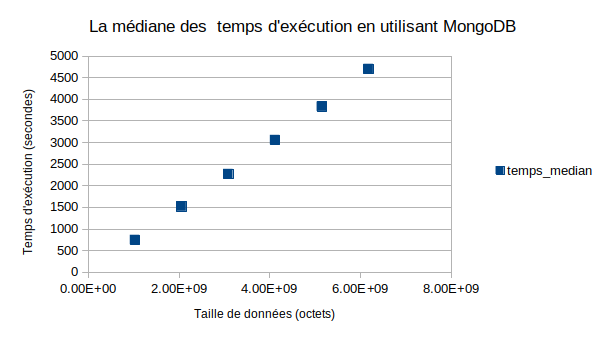
\includegraphics[width=0.7\linewidth]{illustrations/medianTime-execution-mongodb}
	\caption{Le temps d'exécution selon la taille des données avec MongoDB}
	\label{fig:mongodbtiming}
\end{figure}


%D'un test au test suivant, on ajoute les traceroutes d'une journée. Le temps qui s'est ajouté en élargissant l'échantillon de traceroutes  est respectivement  773.08, 753.59, 786.67, 771.99, 871.48. 



%Tandis que la  Figure \ref{fig:mongodbtiming}	 reprend la médiane  des temps d'exécution de la détection en fonction de  la taille de données analysées en utilisant MongoDB. 
%La Figure 	 \ref{fig:moustachemongodb} illustre la variation de la distribution des temps d'exécution. La Figure 	 \ref{fig:moustachemongodb} ainsi que la Figure \ref{fig:mongodbtiming} ont été obtenues en considérant les temps d'exécution de $10$ essais pour chaque taille de données.




%\begin{figure}[h]
%	\centering
%		\captionsetup{justification=centering}
%	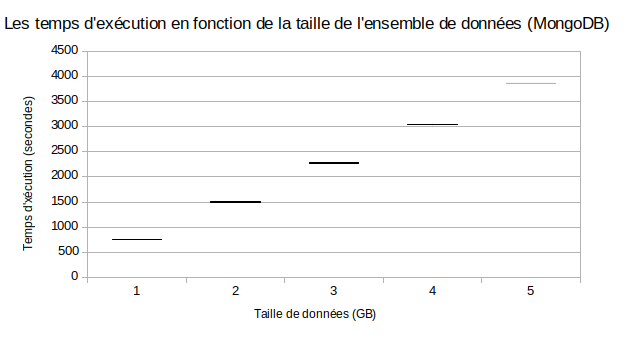
\includegraphics[width=0.7\linewidth]{illustrations/moustacheMongodb_0}
%	\caption{Les temps d'exécution en fonction de la taille de traceroutes analysés (MongoDB)}
%	\label{fig:moustachemongodb}
%\end{figure}

%La variation des temps d'exécution en fonction du nombre de traceroutes 


%Nous évaluons les temps d'exécution lors de l'analyse des délais des liens présents dans un ensemble de traceroutes, en utilisant MongoDB comme technologie de stockage de données massives.   

%On distingue deux types de variations : la taille de l'ensemble de données en terme de stockage et la taille en nombre de traceroutes présents dans l'ensemble de données.

%\begin{table}[h]
%	\captionsetup{justification=centering}
%	\resizebox{1\textwidth}{!}{
%		\begin{tabular}{cccccccc}
%			\textbf{Période}&\textbf{Taille (bytes)}&\textbf{Essai 1 (s)}&\textbf{Essai 2 (s)} %&\textbf{Essai 3 (s)}&\textbf{Essai 4 (s)}&\textbf{Essai 5 (s)}&\textbf{Médiane (s)} \\ %\hline
%			$ 07/02/18 - 07/02/18 $&$  1,028,343,572 $&$ 752,03 $&$ 750 $&$ 755,24 $ &&&\\ \hline 
%			$ 07/02/2018 - 08/02/2018 $&$ 2 $&$ 1499,28 $&$ 1504,98 $&$ 1503,62 $ &&&\\ \hline 
%			$ 07/02/2018 - 09/02/2018 $&$ 3 $&$ 2275,89 $&$2265,96 $&$ 2284,98 $ &&&\\ \hline 
%			$ 07/02/2018 - 10/02/2018 $&$ 4 $&$ 3035,19 $&$ 3043,21 $&$ 3057,45 $&&&\\ \hline 
%			$ 07/02/2018 - 11/02/2018 $&$ 5 $&$ 3871 $&$ 3889,57 $&$ 3894,5 $&&&  \\ \hline 
%		\end{tabular}
%	}
%\section{Application 2 : Amazon DynamoDB}


%\paragraph{Application sur les traceroutes}~


%L'élasticité est une des caractéristiques attirantes des services web d'Amazon. En particulier, c'est le cas d'Amazon DynamoDB. Ainsi, une implémentation basée sur Amazon DynamoDB  n'a pas à se soucier de la capacité  de stockage de données si la quantité de données évolue rapidement. 

 %Amazon DynamoDB  n'assure que le stockage de données dans un processus d'analyse de données. La récupération et le traitement  des données stockées nécessitent l'ajustement des ressources de la machine qui reçoivent ces données, pareillement à MongoDB. La différence se situe à l'évolutivité implicite du stockage de données, qui ne se limite que par la capacité de stockage physique d'AWS. Tandis qu'une installation locale de MongoDB est liée aux ressources de la machine hébergeant ce dernier.  Nous n'avons pas expérimenté Amazon DynamoDB pour analyser les traceroutes, étant donné que notre évaluation des temps d'exécution est effectuée sur une machine locale, nous aurons les mêmes remarques que dans le cas de MongoDB en ce qui concerne l'ajustement des ressources de la machine qui reçoive les données.  
 
% A titre indicatif, une heure de tous les traceroutes effectués par toutes les sondes Atlas, concernant tous les identifiants de mesure,  fait une taille moyenne de  $620$ MB en format compressé, ce que représente une quantité d'environ $9$ GB en format texte.
%Toutefois,  au moment de de la récupération et de la manipulation de ces données, il faut ajuster les ressources pour pouvoir récupérer et traiter une quantité importante de données.


%Avec une autre technologie qui travaille en mémoire, les résultats sont données plus rapidement. 

Nous avons utilisé le volume de traceroutes analysés au lieu du nombre de traceroutes.  Etant donné que le nombre de sauts est différents d'un traceroute à un autre. Les traceroutes ayant plus de sauts nécessitent plus de temps pour être traités. A titre indicatif, la Figure \ref{fig:frequencesauttraceroutes} montre la fréquence des traceroutes ayant le même nombre de sauts. Ces résultats concernent la période entre 07/02/18  et 08/02/18 et l'identifiant de la mesure $ 5004 $.

\begin{figure}[h]
	\centering
	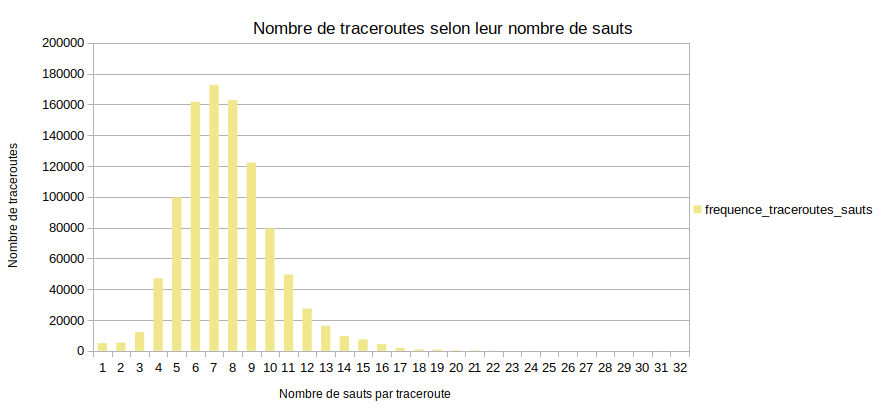
\includegraphics[width=\linewidth]{illustrations/frequencesauttraceroutes2}
	\caption{Fréquence des traceroutes ayant un même nombre de sauts}
	\label{fig:frequencesauttraceroutes}
\end{figure}


\section{Application 2 : Amazon Athena et Amazon S3} 

\paragraph{Performances des services Amazon S3 et Athena dans l'analyse des délais }~ \label{aws-perforsm}


 Notre objectif est de mesurer le temps d'exécution avec  l'intégration des deux services  Amazon S3 et Athena dans l'outil de détection. Cette intégration ne garantit que le stockage des traceroutes. Elle est détaillée dans la section \ref{implementation-athena}. 
La Figure 	\ref{fig:amazonathena} reprend les composantes du temps d'exécution mesuré en se basant sur cette intégration. 
 Selon les paramètres de l'analyse, la requête SQL  est préparée pour que Amazon Athena puisse récupérer les traceroutes depuis Amazon S3. L'interaction avec Amzon Athena est effectuée à travers l'API REST en Python\footnote{Python a été choisi car l'implémentation de référence est écrite en Python.}. Suivant l'état de la requête : succès ou échec, les traitements peuvent être enchaînés sur ces traceroutes incluant les étapes des phases I et II et ce au sein de la machine local. A l'issu de l'analyse de tous les traceroutes, les résultats sont sauvegardés dans un fichier localement.

%On précise que cette intégration envisage la récupération des traceroutes depuis Amason S3 vers la machine de test et ce via Amazon Athena. Le reste des traitements relatifs aux phases I et II sont effectués dans cette machine.   Le temps mesuré concerne la première possibilité décrite dans la section \ref{integration-aws-possibilite-une}. 

\begin{figure}[h]
	\centering
	\captionsetup{justification=centering}
	\resizebox{\textwidth}{!}{
		% Graphic for TeX using PGF
% Title: /home/hayat/RipeAtlasTraceroutesAnalysis/2019/Rapport_Mai/illustrations/amazonathenatiming.dia
% Creator: Dia v0.97+git
% CreationDate: Tue May 28 21:17:53 2019
% For: hayat
% \usepackage{tikz}
% The following commands are not supported in PSTricks at present
% We define them conditionally, so when they are implemented,
% this pgf file will use them.
\ifx\du\undefined
  \newlength{\du}
\fi
\setlength{\du}{15\unitlength}
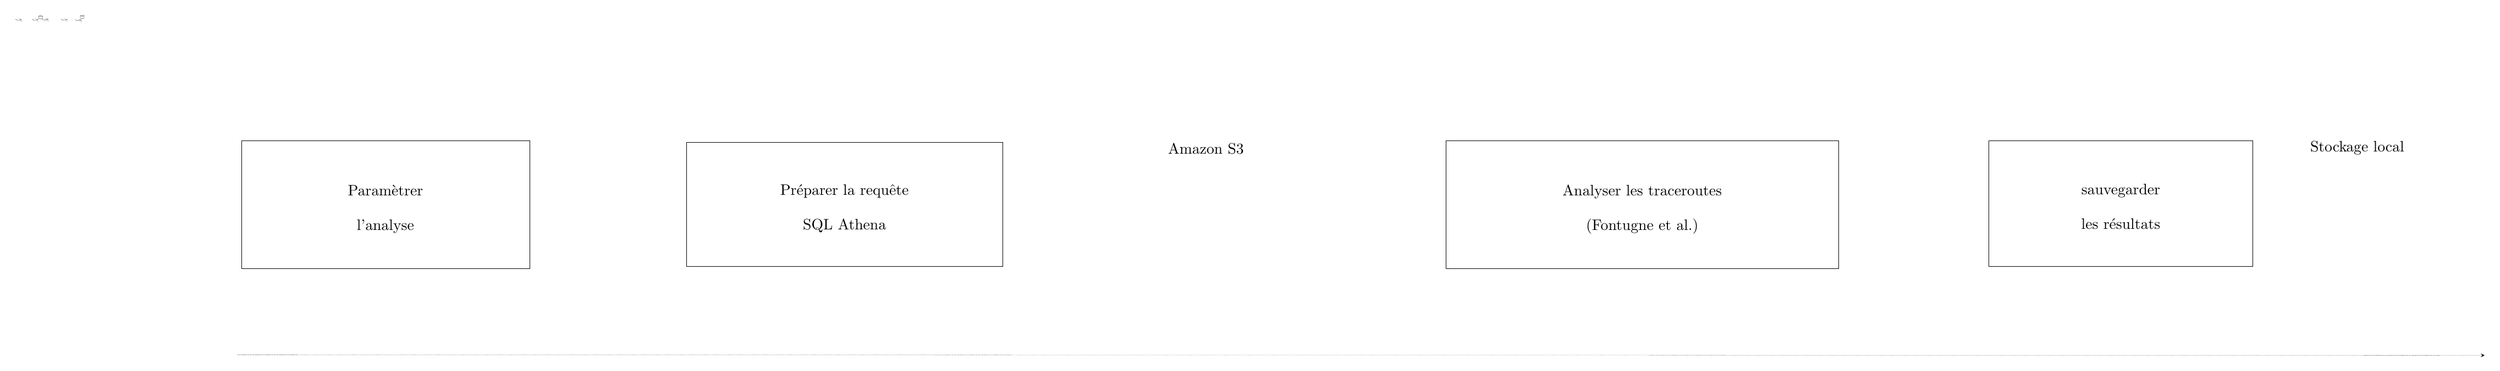
\begin{tikzpicture}[even odd rule]
\pgftransformxscale{1.000000}
\pgftransformyscale{-1.000000}
\definecolor{dialinecolor}{rgb}{0.000000, 0.000000, 0.000000}
\pgfsetstrokecolor{dialinecolor}
\pgfsetstrokeopacity{1.000000}
\definecolor{diafillcolor}{rgb}{1.000000, 1.000000, 1.000000}
\pgfsetfillcolor{diafillcolor}
\pgfsetfillopacity{1.000000}
\pgfsetlinewidth{0.100000\du}
\pgfsetdash{}{0pt}
\pgfsetbuttcap
\pgfsetmiterjoin
\pgfsetlinewidth{0.100000\du}
\pgfsetbuttcap
\pgfsetmiterjoin
\pgfsetdash{}{0pt}
\definecolor{diafillcolor}{rgb}{1.000000, 1.000000, 1.000000}
\pgfsetfillcolor{diafillcolor}
\pgfsetfillopacity{1.000000}
\definecolor{dialinecolor}{rgb}{0.000000, 0.000000, 0.000000}
\pgfsetstrokecolor{dialinecolor}
\pgfsetstrokeopacity{1.000000}
\pgfpathmoveto{\pgfpoint{27.448610\du}{4.301667\du}}
\pgfpathcurveto{\pgfpoint{27.958630\du}{4.026667\du}}{\pgfpoint{28.213640\du}{3.935000\du}}{\pgfpoint{28.723660\du}{3.935000\du}}
\pgfpathcurveto{\pgfpoint{29.233680\du}{3.935000\du}}{\pgfpoint{29.488690\du}{4.026667\du}}{\pgfpoint{29.998710\du}{4.301667\du}}
\pgfpathlineto{\pgfpoint{29.998710\du}{5.768333\du}}
\pgfpathcurveto{\pgfpoint{29.488690\du}{6.043333\du}}{\pgfpoint{29.233680\du}{6.135000\du}}{\pgfpoint{28.723660\du}{6.135000\du}}
\pgfpathcurveto{\pgfpoint{28.213640\du}{6.135000\du}}{\pgfpoint{27.958630\du}{6.043333\du}}{\pgfpoint{27.448610\du}{5.768333\du}}
\pgfpathlineto{\pgfpoint{27.448610\du}{4.301667\du}}
\pgfpathclose
\pgfusepath{fill,stroke}
\pgfsetbuttcap
\pgfsetmiterjoin
\pgfsetdash{}{0pt}
\definecolor{dialinecolor}{rgb}{0.000000, 0.000000, 0.000000}
\pgfsetstrokecolor{dialinecolor}
\pgfsetstrokeopacity{1.000000}
\pgfpathmoveto{\pgfpoint{27.448610\du}{4.301667\du}}
\pgfpathcurveto{\pgfpoint{27.958630\du}{4.576667\du}}{\pgfpoint{28.213640\du}{4.668333\du}}{\pgfpoint{28.723660\du}{4.668333\du}}
\pgfpathcurveto{\pgfpoint{29.233680\du}{4.668333\du}}{\pgfpoint{29.488690\du}{4.576667\du}}{\pgfpoint{29.998710\du}{4.301667\du}}
\pgfusepath{stroke}
% setfont left to latex
\definecolor{dialinecolor}{rgb}{0.000000, 0.000000, 0.000000}
\pgfsetstrokecolor{dialinecolor}
\pgfsetstrokeopacity{1.000000}
\definecolor{diafillcolor}{rgb}{0.000000, 0.000000, 0.000000}
\pgfsetfillcolor{diafillcolor}
\pgfsetfillopacity{1.000000}
\node[anchor=base,inner sep=0pt, outer sep=0pt,color=dialinecolor] at (28.723660\du,5.418333\du){};
% setfont left to latex
\definecolor{dialinecolor}{rgb}{0.000000, 0.000000, 0.000000}
\pgfsetstrokecolor{dialinecolor}
\pgfsetstrokeopacity{1.000000}
\definecolor{diafillcolor}{rgb}{0.000000, 0.000000, 0.000000}
\pgfsetfillcolor{diafillcolor}
\pgfsetfillopacity{1.000000}
\node[anchor=base west,inner sep=0pt,outer sep=0pt,color=dialinecolor] at (27.048610\du,3.335000\du){Amazon S3};
\pgfsetlinewidth{0.100000\du}
\pgfsetdash{{\pgflinewidth}{0.200000\du}}{0cm}
\pgfsetbuttcap
{
\definecolor{diafillcolor}{rgb}{0.000000, 0.000000, 0.000000}
\pgfsetfillcolor{diafillcolor}
\pgfsetfillopacity{1.000000}
% was here!!!
\pgfsetarrowsend{stealth}
\definecolor{dialinecolor}{rgb}{0.000000, 0.000000, 0.000000}
\pgfsetstrokecolor{dialinecolor}
\pgfsetstrokeopacity{1.000000}
\draw (5.545060\du,7.990000\du)--(57.450200\du,8.000000\du);
}
\pgfsetlinewidth{0.100000\du}
\pgfsetdash{}{0pt}
\pgfsetmiterjoin
{\pgfsetcornersarced{\pgfpoint{0.000000\du}{0.000000\du}}\definecolor{diafillcolor}{rgb}{1.000000, 1.000000, 1.000000}
\pgfsetfillcolor{diafillcolor}
\pgfsetfillopacity{1.000000}
\fill (5.645060\du,3.035000\du)--(5.645060\du,5.985000\du)--(12.301110\du,5.985000\du)--(12.301110\du,3.035000\du)--cycle;
}{\pgfsetcornersarced{\pgfpoint{0.000000\du}{0.000000\du}}\definecolor{dialinecolor}{rgb}{0.000000, 0.000000, 0.000000}
\pgfsetstrokecolor{dialinecolor}
\pgfsetstrokeopacity{1.000000}
\draw (5.645060\du,3.035000\du)--(5.645060\du,5.985000\du)--(12.301110\du,5.985000\du)--(12.301110\du,3.035000\du)--cycle;
}% setfont left to latex
\definecolor{dialinecolor}{rgb}{0.000000, 0.000000, 0.000000}
\pgfsetstrokecolor{dialinecolor}
\pgfsetstrokeopacity{1.000000}
\definecolor{diafillcolor}{rgb}{0.000000, 0.000000, 0.000000}
\pgfsetfillcolor{diafillcolor}
\pgfsetfillopacity{1.000000}
\node[anchor=base,inner sep=0pt, outer sep=0pt,color=dialinecolor] at (8.973085\du,4.305000\du){Paramètrer};
% setfont left to latex
\definecolor{dialinecolor}{rgb}{0.000000, 0.000000, 0.000000}
\pgfsetstrokecolor{dialinecolor}
\pgfsetstrokeopacity{1.000000}
\definecolor{diafillcolor}{rgb}{0.000000, 0.000000, 0.000000}
\pgfsetfillcolor{diafillcolor}
\pgfsetfillopacity{1.000000}
\node[anchor=base,inner sep=0pt, outer sep=0pt,color=dialinecolor] at (8.973085\du,5.105000\du){l'analyse};
\pgfsetlinewidth{0.100000\du}
\pgfsetdash{}{0pt}
\pgfsetbuttcap
{
\definecolor{diafillcolor}{rgb}{0.000000, 0.000000, 0.000000}
\pgfsetfillcolor{diafillcolor}
\pgfsetfillopacity{1.000000}
% was here!!!
\pgfsetarrowsend{to}
\definecolor{dialinecolor}{rgb}{0.000000, 0.000000, 0.000000}
\pgfsetstrokecolor{dialinecolor}
\pgfsetstrokeopacity{1.000000}
\pgfpathmoveto{\pgfpoint{12.098564\du}{6.284867\du}}
\pgfpatharc{133}{47}{2.963155\du and 2.963155\du}
\pgfusepath{stroke}
}
\pgfsetlinewidth{0.100000\du}
\pgfsetdash{}{0pt}
\pgfsetmiterjoin
{\pgfsetcornersarced{\pgfpoint{0.000000\du}{0.000000\du}}\definecolor{diafillcolor}{rgb}{1.000000, 1.000000, 1.000000}
\pgfsetfillcolor{diafillcolor}
\pgfsetfillopacity{1.000000}
\fill (33.462410\du,3.035000\du)--(33.462410\du,5.985000\du)--(42.532410\du,5.985000\du)--(42.532410\du,3.035000\du)--cycle;
}{\pgfsetcornersarced{\pgfpoint{0.000000\du}{0.000000\du}}\definecolor{dialinecolor}{rgb}{0.000000, 0.000000, 0.000000}
\pgfsetstrokecolor{dialinecolor}
\pgfsetstrokeopacity{1.000000}
\draw (33.462410\du,3.035000\du)--(33.462410\du,5.985000\du)--(42.532410\du,5.985000\du)--(42.532410\du,3.035000\du)--cycle;
}% setfont left to latex
\definecolor{dialinecolor}{rgb}{0.000000, 0.000000, 0.000000}
\pgfsetstrokecolor{dialinecolor}
\pgfsetstrokeopacity{1.000000}
\definecolor{diafillcolor}{rgb}{0.000000, 0.000000, 0.000000}
\pgfsetfillcolor{diafillcolor}
\pgfsetfillopacity{1.000000}
\node[anchor=base,inner sep=0pt, outer sep=0pt,color=dialinecolor] at (37.997410\du,4.305000\du){Analyser les traceroutes };
% setfont left to latex
\definecolor{dialinecolor}{rgb}{0.000000, 0.000000, 0.000000}
\pgfsetstrokecolor{dialinecolor}
\pgfsetstrokeopacity{1.000000}
\definecolor{diafillcolor}{rgb}{0.000000, 0.000000, 0.000000}
\pgfsetfillcolor{diafillcolor}
\pgfsetfillopacity{1.000000}
\node[anchor=base,inner sep=0pt, outer sep=0pt,color=dialinecolor] at (37.997410\du,5.105000\du){(Fontugne et al.)};
\pgfsetlinewidth{0.100000\du}
\pgfsetdash{}{0pt}
\pgfsetmiterjoin
{\pgfsetcornersarced{\pgfpoint{0.000000\du}{0.000000\du}}\definecolor{diafillcolor}{rgb}{1.000000, 1.000000, 1.000000}
\pgfsetfillcolor{diafillcolor}
\pgfsetfillopacity{1.000000}
\fill (46.002460\du,3.035000\du)--(46.002460\du,5.933955\du)--(52.095060\du,5.933955\du)--(52.095060\du,3.035000\du)--cycle;
}{\pgfsetcornersarced{\pgfpoint{0.000000\du}{0.000000\du}}\definecolor{dialinecolor}{rgb}{0.000000, 0.000000, 0.000000}
\pgfsetstrokecolor{dialinecolor}
\pgfsetstrokeopacity{1.000000}
\draw (46.002460\du,3.035000\du)--(46.002460\du,5.933955\du)--(52.095060\du,5.933955\du)--(52.095060\du,3.035000\du)--cycle;
}% setfont left to latex
\definecolor{dialinecolor}{rgb}{0.000000, 0.000000, 0.000000}
\pgfsetstrokecolor{dialinecolor}
\pgfsetstrokeopacity{1.000000}
\definecolor{diafillcolor}{rgb}{0.000000, 0.000000, 0.000000}
\pgfsetfillcolor{diafillcolor}
\pgfsetfillopacity{1.000000}
\node[anchor=base,inner sep=0pt, outer sep=0pt,color=dialinecolor] at (49.048760\du,4.279477\du){sauvegarder };
% setfont left to latex
\definecolor{dialinecolor}{rgb}{0.000000, 0.000000, 0.000000}
\pgfsetstrokecolor{dialinecolor}
\pgfsetstrokeopacity{1.000000}
\definecolor{diafillcolor}{rgb}{0.000000, 0.000000, 0.000000}
\pgfsetfillcolor{diafillcolor}
\pgfsetfillopacity{1.000000}
\node[anchor=base,inner sep=0pt, outer sep=0pt,color=dialinecolor] at (49.048760\du,5.079477\du){les résultats};
\pgfsetlinewidth{0.100000\du}
\pgfsetdash{}{0pt}
\pgfsetbuttcap
{
\definecolor{diafillcolor}{rgb}{0.000000, 0.000000, 0.000000}
\pgfsetfillcolor{diafillcolor}
\pgfsetfillopacity{1.000000}
% was here!!!
\pgfsetarrowsend{to}
\definecolor{dialinecolor}{rgb}{0.000000, 0.000000, 0.000000}
\pgfsetstrokecolor{dialinecolor}
\pgfsetstrokeopacity{1.000000}
\pgfpathmoveto{\pgfpoint{23.044178\du}{6.275480\du}}
\pgfpatharc{133}{47}{2.963155\du and 2.963155\du}
\pgfusepath{stroke}
}
\pgfsetlinewidth{0.100000\du}
\pgfsetdash{}{0pt}
\pgfsetbuttcap
{
\definecolor{diafillcolor}{rgb}{0.000000, 0.000000, 0.000000}
\pgfsetfillcolor{diafillcolor}
\pgfsetfillopacity{1.000000}
% was here!!!
\pgfsetarrowsend{to}
\definecolor{dialinecolor}{rgb}{0.000000, 0.000000, 0.000000}
\pgfsetstrokecolor{dialinecolor}
\pgfsetstrokeopacity{1.000000}
\pgfpathmoveto{\pgfpoint{42.194178\du}{6.275480\du}}
\pgfpatharc{133}{47}{2.963155\du and 2.963155\du}
\pgfusepath{stroke}
}
\pgfsetlinewidth{0.100000\du}
\pgfsetdash{}{0pt}
\pgfsetbuttcap
{
\definecolor{diafillcolor}{rgb}{0.000000, 0.000000, 0.000000}
\pgfsetfillcolor{diafillcolor}
\pgfsetfillopacity{1.000000}
% was here!!!
\pgfsetarrowsend{to}
\definecolor{dialinecolor}{rgb}{0.000000, 0.000000, 0.000000}
\pgfsetstrokecolor{dialinecolor}
\pgfsetstrokeopacity{1.000000}
\pgfpathmoveto{\pgfpoint{29.599120\du}{6.140480\du}}
\pgfpatharc{133}{47}{2.963155\du and 2.963155\du}
\pgfusepath{stroke}
}
\pgfsetlinewidth{0.100000\du}
\pgfsetdash{}{0pt}
\pgfsetmiterjoin
{\pgfsetcornersarced{\pgfpoint{0.000000\du}{0.000000\du}}\definecolor{diafillcolor}{rgb}{1.000000, 1.000000, 1.000000}
\pgfsetfillcolor{diafillcolor}
\pgfsetfillopacity{1.000000}
\fill (15.928602\du,3.065000\du)--(15.928602\du,5.940000\du)--(23.221102\du,5.940000\du)--(23.221102\du,3.065000\du)--cycle;
}{\pgfsetcornersarced{\pgfpoint{0.000000\du}{0.000000\du}}\definecolor{dialinecolor}{rgb}{0.000000, 0.000000, 0.000000}
\pgfsetstrokecolor{dialinecolor}
\pgfsetstrokeopacity{1.000000}
\draw (15.928602\du,3.065000\du)--(15.928602\du,5.940000\du)--(23.221102\du,5.940000\du)--(23.221102\du,3.065000\du)--cycle;
}% setfont left to latex
\definecolor{dialinecolor}{rgb}{0.000000, 0.000000, 0.000000}
\pgfsetstrokecolor{dialinecolor}
\pgfsetstrokeopacity{1.000000}
\definecolor{diafillcolor}{rgb}{0.000000, 0.000000, 0.000000}
\pgfsetfillcolor{diafillcolor}
\pgfsetfillopacity{1.000000}
\node[anchor=base,inner sep=0pt, outer sep=0pt,color=dialinecolor] at (19.574852\du,4.297500\du){Préparer la requête};
% setfont left to latex
\definecolor{dialinecolor}{rgb}{0.000000, 0.000000, 0.000000}
\pgfsetstrokecolor{dialinecolor}
\pgfsetstrokeopacity{1.000000}
\definecolor{diafillcolor}{rgb}{0.000000, 0.000000, 0.000000}
\pgfsetfillcolor{diafillcolor}
\pgfsetfillopacity{1.000000}
\node[anchor=base,inner sep=0pt, outer sep=0pt,color=dialinecolor] at (19.574852\du,5.097500\du){ SQL Athena};
\pgfsetlinewidth{0.100000\du}
\pgfsetdash{}{0pt}
\pgfsetbuttcap
\pgfsetmiterjoin
\pgfsetlinewidth{0.100000\du}
\pgfsetbuttcap
\pgfsetmiterjoin
\pgfsetdash{}{0pt}
\definecolor{diafillcolor}{rgb}{1.000000, 1.000000, 1.000000}
\pgfsetfillcolor{diafillcolor}
\pgfsetfillopacity{1.000000}
\definecolor{dialinecolor}{rgb}{0.000000, 0.000000, 0.000000}
\pgfsetstrokecolor{dialinecolor}
\pgfsetstrokeopacity{1.000000}
\pgfpathmoveto{\pgfpoint{54.775200\du}{4.101667\du}}
\pgfpathcurveto{\pgfpoint{55.285220\du}{3.826667\du}}{\pgfpoint{55.540230\du}{3.735000\du}}{\pgfpoint{56.050250\du}{3.735000\du}}
\pgfpathcurveto{\pgfpoint{56.560270\du}{3.735000\du}}{\pgfpoint{56.815280\du}{3.826667\du}}{\pgfpoint{57.325300\du}{4.101667\du}}
\pgfpathlineto{\pgfpoint{57.325300\du}{5.568333\du}}
\pgfpathcurveto{\pgfpoint{56.815280\du}{5.843333\du}}{\pgfpoint{56.560270\du}{5.935000\du}}{\pgfpoint{56.050250\du}{5.935000\du}}
\pgfpathcurveto{\pgfpoint{55.540230\du}{5.935000\du}}{\pgfpoint{55.285220\du}{5.843333\du}}{\pgfpoint{54.775200\du}{5.568333\du}}
\pgfpathlineto{\pgfpoint{54.775200\du}{4.101667\du}}
\pgfpathclose
\pgfusepath{fill,stroke}
\pgfsetbuttcap
\pgfsetmiterjoin
\pgfsetdash{}{0pt}
\definecolor{dialinecolor}{rgb}{0.000000, 0.000000, 0.000000}
\pgfsetstrokecolor{dialinecolor}
\pgfsetstrokeopacity{1.000000}
\pgfpathmoveto{\pgfpoint{54.775200\du}{4.101667\du}}
\pgfpathcurveto{\pgfpoint{55.285220\du}{4.376667\du}}{\pgfpoint{55.540230\du}{4.468333\du}}{\pgfpoint{56.050250\du}{4.468333\du}}
\pgfpathcurveto{\pgfpoint{56.560270\du}{4.468333\du}}{\pgfpoint{56.815280\du}{4.376667\du}}{\pgfpoint{57.325300\du}{4.101667\du}}
\pgfusepath{stroke}
% setfont left to latex
\definecolor{dialinecolor}{rgb}{0.000000, 0.000000, 0.000000}
\pgfsetstrokecolor{dialinecolor}
\pgfsetstrokeopacity{1.000000}
\definecolor{diafillcolor}{rgb}{0.000000, 0.000000, 0.000000}
\pgfsetfillcolor{diafillcolor}
\pgfsetfillopacity{1.000000}
\node[anchor=base,inner sep=0pt, outer sep=0pt,color=dialinecolor] at (56.050250\du,5.218333\du){};
% setfont left to latex
\definecolor{dialinecolor}{rgb}{0.000000, 0.000000, 0.000000}
\pgfsetstrokecolor{dialinecolor}
\pgfsetstrokeopacity{1.000000}
\definecolor{diafillcolor}{rgb}{0.000000, 0.000000, 0.000000}
\pgfsetfillcolor{diafillcolor}
\pgfsetfillopacity{1.000000}
\node[anchor=base west,inner sep=0pt,outer sep=0pt,color=dialinecolor] at (53.425200\du,3.285000\du){Stockage local};
\pgfsetlinewidth{0.100000\du}
\pgfsetdash{}{0pt}
\pgfsetbuttcap
{
\definecolor{diafillcolor}{rgb}{0.000000, 0.000000, 0.000000}
\pgfsetfillcolor{diafillcolor}
\pgfsetfillopacity{1.000000}
% was here!!!
\pgfsetarrowsend{to}
\definecolor{dialinecolor}{rgb}{0.000000, 0.000000, 0.000000}
\pgfsetstrokecolor{dialinecolor}
\pgfsetstrokeopacity{1.000000}
\pgfpathmoveto{\pgfpoint{51.375668\du}{6.540480\du}}
\pgfpatharc{133}{47}{2.963155\du and 2.963155\du}
\pgfusepath{stroke}
}
\end{tikzpicture}

	}
	\caption{Les composantes du temps d'exécution lors de l'analyse des traceroutes avec Amazon S3 et Athena }
	\label{fig:amazonathena}
\end{figure}


%Nous avons utilisé Amazon Athena et Amazon S3 pour analyser les traceroutes et détecter les anomalies des délais.


%L'interaction avec Amazon Athena a été fait   en utilisant l'API REST  en Python, car l'implémentation proposée par les auteurs du travail de référence est écrite en Python. Ceci facilite l'intégration de ces services dans l'implémentation.

%nous avons adapté cette implémentation de sorte  de récupérer les traceroutes depuis   depuis Amazon S3 via Amazon Athena au   lieu de le faire depuis la base de données locale MongoDB.  

Etant donné que nous avons utilisé le partitionnement de données, la préparation de la requête SQL 
doit prendre en compte le choix des partitions à consulter selon les données souhaitées.
Les paramètres de l'outil de détection permettent d'avoir  la date de début et de fin. Ceci permet d'inférer toutes les périodes de l'analyse. Ainsi, pour chaque période, on a les informations relatives aux partitions suivantes  : \textit{year}, \textit{month} et \textit{day}. Les paramètres de l'analyse ont été adaptés pour prendre en compte les identifiants de mesures lors de la préparation de la requête SQL. Si des identifiants de mesures sont indiqués, les partitions concernées sont considérées. Or, si ce n'est pas le cas, toutes les mesures sont analysées sans exception.

%qui indiquent les traceroutes à considérer. 

%Or, avec l'utilisation du partitionnement, on peut encore  préciser les traceroutes en se limitant à une ou plusieurs   mesures Atlas. 
%La requête SQL présentée dans la Figure 	\ref{fig:sqlrequestathena} montre un exemple où on se limite aux traceroutes en provenance des mesures $ 5001 $ et $ 5004 $.
 
%une analyse des délais nécessite d'autres paramètres à ajuster en plus de ceux relatifs à la détection. Ce sont les paramètres permettant de sélectionner les traceroutes présents sur Amazon S3. Du fait que le partitionnement de données (voir une partie de l'arborescence dans la Figure 	\ref{fig:partitionnement-athena}) est réalisé sur base du type de traceroute (\textit{builtin} ou \textit{anchor}) et de l'identifiant de la mesure ($ 5004 $, $6001$, etc) qui a enregistré un traceroute, nous devons personnaliser  la requête visant la   récupération des traceroutes  depuis Amazon S3 pour qu'elle prennent en compte aussi les partitions.

Le Tableau \ref{tab:athena-data} montre les temps d'exécution obtenus lors de deux essais selon la taille de l'ensemble de traceroutes analysés et le temps médian de ces deux temps.

\begin{table}[h]
	\centering
	\captionsetup{justification=centering}
	\resizebox{\textwidth}{!}{
\begin{tabular}{c c ccc}
	\textbf{Période (début - fin)} & \textbf{Taille(octets)} & \textbf{Essai 1 (secondes) }&\textbf{Essai 2 (secondes) } & \textbf{Médiane (secondes)} \\ 	\hline 
$ 07/02/18 - 07/02/18 $	&$ 1028343572 $&	$ 1898.31 $  &$1766.13$ &$ 1832.22 $\\ 	\hline 
$ 07/02/18 - 08/02/18 $	&$ 2055167238 $&	$ 3533.65 $ &$ 3622.10 $ & $3577.88$\\ 	\hline 
$ 07/02/18 - 09/02/18 $&	$ 3083779157 $&	$ 5284.91  $ & $ 5415.67 $ & $5350.29$\\ 	\hline 
$ 07/02/18 - 10/02/18 $	&$ 4113776434 $&$ 	7228.88 $ &$ 7658.80 $ & $7443.84$  \\ 	\hline 
$ 07/02/18 - 11/02/18 $	&$ 5143831662 $& $ 8984.87	 $ &$ 9245.56 $  & $9115.21$\\ 	\hline 
\end{tabular} 
}
\caption{Les temps d'exécution par taille de l'ensemble de données (Amazon Athena et Amazon S3)}
\label{tab:athena-data}
\end{table}






Le temps d'exécution calculé concerne trois phases principales. Premièrement,  les données sont récupérées depuis Amazon S3. Plusieurs facteurs affectent cette étape. Par exemple,  les conditions du réseau, les ressources allouées par Amazon pour répondre à chaque requête  Athena à destination des données disponibles sur Amazon S3, l'optimalité de la requête SQL, etc.
En deuxième lieu, les résultats de la requête doivent être désérialisés pour pouvoir les utiliser localement. Enfin, sur base des données récupérées, les phases I et II peuvent être effectuées. Les résultats obtenus sont stockés dans un fichier localement.
%
%
%Nous évaluons les temps d'exécution de plusieurs  analyses de délais lancées en variant la taille de données. Rappelons qu'il s'agit de la première possibilité: Amazon S3 pour le stockage de traceroutes et Amazon Athena pour récupérer les traceroutes valides, le reste de traitements sont effectués au sein de la machine locale.  Le Tableau	\ref{tab:awstiming-timing} reprend plus de détails. 
%\begin{table}[H]
%	%\begin{threeparttable}
%	
%	\captionsetup{justification=centering}
%	\begin{tabular}{ccccc}
%		\textbf{Début - fin} &\textbf{Durée (jours)}  & \textbf{Taille}  & \textbf{Nb traceroutes} & \textbf{Temps (secondes)} \\ \hline
%		
%		07/02/2018             &1 &1 GB&& 3870\\ \hline
%		07/02/2018 - 08/02/2018&2 &1 GB&& 2942\\ \hline
%		07/02/2018 - 09/02/2018&3 & 1 GB&& 2991\\ \hline
%		07/02/2018 - 10/02/2018&4 & 3 GB&& 20955\\ \hline
%		07/02/2018 - 11/02/2018&5& && \\ \hline
%		07/02/2018 - 12/02/2018&6& && \\ \hline
%		07/02/2018 - 13/02/2018&7& && \\ \hline
%		07/02/2018 - 14/02/2018&8& && \\ \hline
%		07/02/2018 - 15/02/2018&9& && \\ \hline
%		07/02/2018 - 16/02/2018&10& && \\ \hline
%		07/02/2018 - 17/02/2018&11& && \\ \hline
%		07/02/2018 - 18/02/2018&12& && \\ \hline
%		07/02/2018 - 19/02/2018&13& && \\ \hline
%		07/02/2018 - 20/02/2018&14& && \\ \hline
%	\end{tabular}
%	\caption{La moyenne des temps d'exécution d'analyse de traceroutes en fonction de la taille de données avec Amazon S3 et Amazon Athena }
%	\label{tab:awstiming-timing}
%\end{table}
La Figure \ref{fig:temps-avec-aws} présente graphiquement le temps médian des deux  essais pour chacune des tailles utilisées auparavant avec MongoDB. 

% Le temps de chaque essai comprend l'étape de la récupération des traceroutes depuis Amazon S3, le temps de préparation des traceroute et enfin le temps de la détection des anomalies. Autrement dit, le temps nécessaire à la réalisation des phases I, II et celui nécessaire pour sauvegarder les résultats par lien.

\begin{figure}[h]
	\centering
	\captionsetup{justification=centering}
	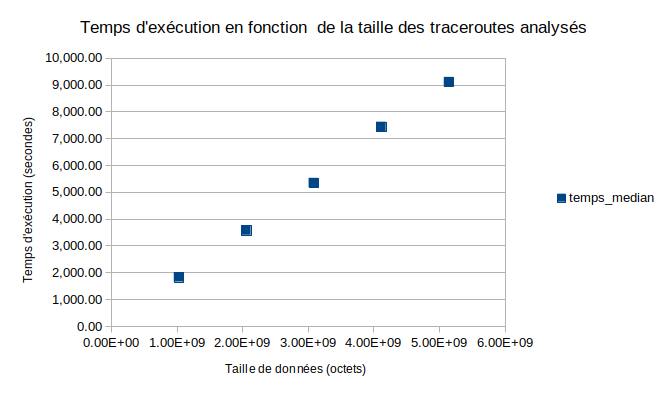
\includegraphics[width=\linewidth]{illustrations/temps-exection-amazonathena}
	\caption{Les temps d'exécution de la détection des anomalies en fonction de la taille de données (Amazon S3 et Amazon Athena)}
	\label{fig:temps-avec-aws}
\end{figure}


Le temps d'exécution obtenu lors de l'utilisation des services Amazon S3 et Athena dépendent du temps nécessaire pour recevoir la réponse à la requête SQL. Avec l'intégration proposée, l'analyse des traceroutes est effectuée par périodes d'une heure et les traceroutes sont stockées par journée. On compte une requête SQL vers Amazon Athena pour chaque période. 
A chaque période, une requête SQL est préparée pour chercher les traceroutes  dans les partitions  correspondantes. Le temps de réponse aux requêtes SQL sur Amazon Athena peut être calculé en utilisant l'API d'Athena en Python ou bien à travers la console d'Athena.  


Afin de mesurer l'effet du partitionnement sur le temps de l'analyse ainsi que pour avoir une idée sur une des composantes affectant les temps obtenus dans le Tableau \ref{tab:athena-data}, nous avons évalué dans  Le Tableau \ref{datatimeathenaconsole}  le temps écoulé pour récupérer les traceroutes effectués durant une heure,  en provenance de l'identifiant de la mesure $5004$ (msm='5004'), concernant l'année (year='2018') et le mois (month='2'). Pour les jours (partition day), elles sont variées et données dans le Tableau   \ref{datatimeathenaconsole}.
Ce dernier reprend le temps d'exécution de la requête SQL et les données analysées selon les valeurs de la partition \textit{day}.
\begin{table}[h]
	\captionsetup{justification=centering}
	\centering
		\resizebox{1\textwidth}{!}{
\begin{tabular}{c c l}
\textbf{Temps d'exécution (secondes)}&	\textbf{Taille de données (MO)}& \multicolumn{1}{c}{ \textbf{Partitions : day}}  \\ \hline
	$ 29.38 $&	$ 96.81 $ & '7'\\ \hline
	$ 31.15 $&	$ 203.2 $ & '7' or '8' \\ \hline
	$ 31.43 $&	$ 309.78 $ &  '7' or  '8' or 9\\ \hline
	$ 29.88 $&	$ 416.5 $  & '7' or  '8' or 9 or 10\\ \hline
	$ 31.27 $&	$ 523.23 $ & '7' or  '8' or 9 or 10 or '11'\\ \hline
	$ 49.91 $&	$ 618.93 $ & '7' or  '8' or 9 or 10 or '11' or '27'\\ \hline
\end{tabular} 
}
\caption{Les temps d'exécution d'une requête SQL sur Amazon Athena selon les données analysées}
\label{datatimeathenaconsole}
\end{table}


%Nous précisons qu'une même requête exécutée depuis la console d'Amazon Athena est exécutée plus rapidement qu'une requête exécutée en utilisant l'API en Python. 


Si le temps se diffère selon les données analysées. Ce même temps est différent aussi si cette requête est exécutées depuis la console d'Athena ou via l'API. Par exemple, une même requête SQL a été exécutée depuis la console d'Athena  en $ 29.38 $ secondes et en $ 67.45 $ secondes depuis l'API.






\section{Application 3 : Apache Spark  avec Scala}
Nous avons implémenté l'outil de détection avec le framework Spark et l'API Scala. Les détails de l'implémentation sont donnés dans la section \ref{application:spark}.  Nous avons évalué le temps d'exécution de l'outil de détection en analysant différents échantillons de traceroutes  en mode local et en mode \textit{cluster}. Pour le mode local, nous avons lancé l'application Spark sur la machine ayant les caractéristiques  reprises dans la section \ref{machine-openvz-caracteritics}. Pour le mode \textit{cluster}, nous avons utilisé le \textit{cluster} EMR et nous donnons les caractéristiques techniques du \textit{cluster} utilisé pour chaque test.


\subsection{Mode local}

A la base Spark est conçu pour être utilisé dans un \textit{cluster} de machines sur  lequel l'analyse de données est distribuée. Toutefois, Spark peut être utilisé en mode local. Dans ce mode, on trouve le \textit{driver} et un seul \textit{executor}. Ce dernier est "lié" au même processus initié par le \textit{driver}. 


%\paragraph{Performances d'Apache Spark dans l'analyse des délais }~
%Nous avons évalué le temps d'exécution de l'implémentation de l'outil de détection en utilisant Spark en variant le nombre de traceroutes à analyser. Nous avons aussi varié certains paramètres relatifs à la soumission de l'application au Spark. Nous avons varié la taille de la mémoire allouée au driver afin de choisir celle la plus adaptée. Ensuite nous avons mesuré le temps d'exécution dans le cas de local, local[K] et local[*].

La Figure \ref{fig:sparktimingLocal} illustre les principales étapes de l'analyse des traceroutes en utilisant Spark et Scala en mode local. Selon les paramètres de l'analyse et les paramètres du Spark, la commande permettant la soumission l'application Spark est préparée. A la soumission de l'application, les données à analyser sont lues depuis l'endroit local. Après avoir traité tous les traceroutes en effectuant les étapes de la phase I et II, les résultats obtenus pour chaque lien sont sauvegardés localement. 

\begin{figure}[H]
	\centering
	\captionsetup{justification=centering}
	\resizebox{\textwidth}{!}{
		% Graphic for TeX using PGF
% Title: /home/hayat/RipeAtlasTraceroutesAnalysis/2019/Rapport_Mai/illustrations/sparktimingLocal.dia
% Creator: Dia v0.97+git
% CreationDate: Sun Jun  2 20:08:55 2019
% For: hayat
% \usepackage{tikz}
% The following commands are not supported in PSTricks at present
% We define them conditionally, so when they are implemented,
% this pgf file will use them.
\ifx\du\undefined
  \newlength{\du}
\fi
\setlength{\du}{15\unitlength}
\begin{tikzpicture}[even odd rule]
\pgftransformxscale{1.000000}
\pgftransformyscale{-1.000000}
\definecolor{dialinecolor}{rgb}{0.000000, 0.000000, 0.000000}
\pgfsetstrokecolor{dialinecolor}
\pgfsetstrokeopacity{1.000000}
\definecolor{diafillcolor}{rgb}{1.000000, 1.000000, 1.000000}
\pgfsetfillcolor{diafillcolor}
\pgfsetfillopacity{1.000000}
\pgfsetlinewidth{0.100000\du}
\pgfsetdash{}{0pt}
\pgfsetbuttcap
\pgfsetmiterjoin
\pgfsetlinewidth{0.100000\du}
\pgfsetbuttcap
\pgfsetmiterjoin
\pgfsetdash{}{0pt}
\definecolor{diafillcolor}{rgb}{1.000000, 1.000000, 1.000000}
\pgfsetfillcolor{diafillcolor}
\pgfsetfillopacity{1.000000}
\definecolor{dialinecolor}{rgb}{0.000000, 0.000000, 0.000000}
\pgfsetstrokecolor{dialinecolor}
\pgfsetstrokeopacity{1.000000}
\pgfpathmoveto{\pgfpoint{25.498600\du}{4.101667\du}}
\pgfpathcurveto{\pgfpoint{26.008620\du}{3.826667\du}}{\pgfpoint{26.263630\du}{3.735000\du}}{\pgfpoint{26.773650\du}{3.735000\du}}
\pgfpathcurveto{\pgfpoint{27.283670\du}{3.735000\du}}{\pgfpoint{27.538680\du}{3.826667\du}}{\pgfpoint{28.048700\du}{4.101667\du}}
\pgfpathlineto{\pgfpoint{28.048700\du}{5.568333\du}}
\pgfpathcurveto{\pgfpoint{27.538680\du}{5.843333\du}}{\pgfpoint{27.283670\du}{5.935000\du}}{\pgfpoint{26.773650\du}{5.935000\du}}
\pgfpathcurveto{\pgfpoint{26.263630\du}{5.935000\du}}{\pgfpoint{26.008620\du}{5.843333\du}}{\pgfpoint{25.498600\du}{5.568333\du}}
\pgfpathlineto{\pgfpoint{25.498600\du}{4.101667\du}}
\pgfpathclose
\pgfusepath{fill,stroke}
\pgfsetbuttcap
\pgfsetmiterjoin
\pgfsetdash{}{0pt}
\definecolor{dialinecolor}{rgb}{0.000000, 0.000000, 0.000000}
\pgfsetstrokecolor{dialinecolor}
\pgfsetstrokeopacity{1.000000}
\pgfpathmoveto{\pgfpoint{25.498600\du}{4.101667\du}}
\pgfpathcurveto{\pgfpoint{26.008620\du}{4.376667\du}}{\pgfpoint{26.263630\du}{4.468333\du}}{\pgfpoint{26.773650\du}{4.468333\du}}
\pgfpathcurveto{\pgfpoint{27.283670\du}{4.468333\du}}{\pgfpoint{27.538680\du}{4.376667\du}}{\pgfpoint{28.048700\du}{4.101667\du}}
\pgfusepath{stroke}
% setfont left to latex
\definecolor{dialinecolor}{rgb}{0.000000, 0.000000, 0.000000}
\pgfsetstrokecolor{dialinecolor}
\pgfsetstrokeopacity{1.000000}
\definecolor{diafillcolor}{rgb}{0.000000, 0.000000, 0.000000}
\pgfsetfillcolor{diafillcolor}
\pgfsetfillopacity{1.000000}
\node[anchor=base,inner sep=0pt, outer sep=0pt,color=dialinecolor] at (26.773650\du,5.218333\du){};
% setfont left to latex
\definecolor{dialinecolor}{rgb}{0.000000, 0.000000, 0.000000}
\pgfsetstrokecolor{dialinecolor}
\pgfsetstrokeopacity{1.000000}
\definecolor{diafillcolor}{rgb}{0.000000, 0.000000, 0.000000}
\pgfsetfillcolor{diafillcolor}
\pgfsetfillopacity{1.000000}
\node[anchor=base west,inner sep=0pt,outer sep=0pt,color=dialinecolor] at (23.998600\du,3.135000\du){Stockage Local};
\pgfsetlinewidth{0.100000\du}
\pgfsetdash{{\pgflinewidth}{0.200000\du}}{0cm}
\pgfsetbuttcap
{
\definecolor{diafillcolor}{rgb}{0.000000, 0.000000, 0.000000}
\pgfsetfillcolor{diafillcolor}
\pgfsetfillopacity{1.000000}
% was here!!!
\pgfsetarrowsend{stealth}
\definecolor{dialinecolor}{rgb}{0.000000, 0.000000, 0.000000}
\pgfsetstrokecolor{dialinecolor}
\pgfsetstrokeopacity{1.000000}
\draw (18.144900\du,9.950000\du)--(52.945000\du,9.900000\du);
}
\pgfsetlinewidth{0.100000\du}
\pgfsetdash{}{0pt}
\pgfsetmiterjoin
{\pgfsetcornersarced{\pgfpoint{0.000000\du}{0.000000\du}}\definecolor{diafillcolor}{rgb}{1.000000, 1.000000, 1.000000}
\pgfsetfillcolor{diafillcolor}
\pgfsetfillopacity{1.000000}
\fill (18.221100\du,3.035000\du)--(18.221100\du,5.985000\du)--(22.901100\du,5.985000\du)--(22.901100\du,3.035000\du)--cycle;
}{\pgfsetcornersarced{\pgfpoint{0.000000\du}{0.000000\du}}\definecolor{dialinecolor}{rgb}{0.000000, 0.000000, 0.000000}
\pgfsetstrokecolor{dialinecolor}
\pgfsetstrokeopacity{1.000000}
\draw (18.221100\du,3.035000\du)--(18.221100\du,5.985000\du)--(22.901100\du,5.985000\du)--(22.901100\du,3.035000\du)--cycle;
}% setfont left to latex
\definecolor{dialinecolor}{rgb}{0.000000, 0.000000, 0.000000}
\pgfsetstrokecolor{dialinecolor}
\pgfsetstrokeopacity{1.000000}
\definecolor{diafillcolor}{rgb}{0.000000, 0.000000, 0.000000}
\pgfsetfillcolor{diafillcolor}
\pgfsetfillopacity{1.000000}
\node[anchor=base,inner sep=0pt, outer sep=0pt,color=dialinecolor] at (20.561100\du,4.305000\du){Paramètrer};
% setfont left to latex
\definecolor{dialinecolor}{rgb}{0.000000, 0.000000, 0.000000}
\pgfsetstrokecolor{dialinecolor}
\pgfsetstrokeopacity{1.000000}
\definecolor{diafillcolor}{rgb}{0.000000, 0.000000, 0.000000}
\pgfsetfillcolor{diafillcolor}
\pgfsetfillopacity{1.000000}
\node[anchor=base,inner sep=0pt, outer sep=0pt,color=dialinecolor] at (20.561100\du,5.105000\du){l'analyse};
\pgfsetlinewidth{0.100000\du}
\pgfsetdash{}{0pt}
\pgfsetmiterjoin
{\pgfsetcornersarced{\pgfpoint{0.000000\du}{0.000000\du}}\definecolor{diafillcolor}{rgb}{1.000000, 1.000000, 1.000000}
\pgfsetfillcolor{diafillcolor}
\pgfsetfillopacity{1.000000}
\fill (30.112400\du,0.900000\du)--(30.112400\du,3.600000\du)--(39.182400\du,3.600000\du)--(39.182400\du,0.900000\du)--cycle;
}{\pgfsetcornersarced{\pgfpoint{0.000000\du}{0.000000\du}}\definecolor{dialinecolor}{rgb}{0.000000, 0.000000, 0.000000}
\pgfsetstrokecolor{dialinecolor}
\pgfsetstrokeopacity{1.000000}
\draw (30.112400\du,0.900000\du)--(30.112400\du,3.600000\du)--(39.182400\du,3.600000\du)--(39.182400\du,0.900000\du)--cycle;
}% setfont left to latex
\definecolor{dialinecolor}{rgb}{0.000000, 0.000000, 0.000000}
\pgfsetstrokecolor{dialinecolor}
\pgfsetstrokeopacity{1.000000}
\definecolor{diafillcolor}{rgb}{0.000000, 0.000000, 0.000000}
\pgfsetfillcolor{diafillcolor}
\pgfsetfillopacity{1.000000}
\node[anchor=base,inner sep=0pt, outer sep=0pt,color=dialinecolor] at (34.647400\du,2.045000\du){Analyser les traceroutes };
% setfont left to latex
\definecolor{dialinecolor}{rgb}{0.000000, 0.000000, 0.000000}
\pgfsetstrokecolor{dialinecolor}
\pgfsetstrokeopacity{1.000000}
\definecolor{diafillcolor}{rgb}{0.000000, 0.000000, 0.000000}
\pgfsetfillcolor{diafillcolor}
\pgfsetfillopacity{1.000000}
\node[anchor=base,inner sep=0pt, outer sep=0pt,color=dialinecolor] at (34.647400\du,2.845000\du){Spark/Scala};
\pgfsetlinewidth{0.100000\du}
\pgfsetdash{}{0pt}
\pgfsetmiterjoin
{\pgfsetcornersarced{\pgfpoint{0.000000\du}{0.000000\du}}\definecolor{diafillcolor}{rgb}{1.000000, 1.000000, 1.000000}
\pgfsetfillcolor{diafillcolor}
\pgfsetfillopacity{1.000000}
\fill (41.552500\du,3.035000\du)--(41.552500\du,5.933955\du)--(47.645100\du,5.933955\du)--(47.645100\du,3.035000\du)--cycle;
}{\pgfsetcornersarced{\pgfpoint{0.000000\du}{0.000000\du}}\definecolor{dialinecolor}{rgb}{0.000000, 0.000000, 0.000000}
\pgfsetstrokecolor{dialinecolor}
\pgfsetstrokeopacity{1.000000}
\draw (41.552500\du,3.035000\du)--(41.552500\du,5.933955\du)--(47.645100\du,5.933955\du)--(47.645100\du,3.035000\du)--cycle;
}% setfont left to latex
\definecolor{dialinecolor}{rgb}{0.000000, 0.000000, 0.000000}
\pgfsetstrokecolor{dialinecolor}
\pgfsetstrokeopacity{1.000000}
\definecolor{diafillcolor}{rgb}{0.000000, 0.000000, 0.000000}
\pgfsetfillcolor{diafillcolor}
\pgfsetfillopacity{1.000000}
\node[anchor=base,inner sep=0pt, outer sep=0pt,color=dialinecolor] at (44.598800\du,4.279477\du){sauvegarder };
% setfont left to latex
\definecolor{dialinecolor}{rgb}{0.000000, 0.000000, 0.000000}
\pgfsetstrokecolor{dialinecolor}
\pgfsetstrokeopacity{1.000000}
\definecolor{diafillcolor}{rgb}{0.000000, 0.000000, 0.000000}
\pgfsetfillcolor{diafillcolor}
\pgfsetfillopacity{1.000000}
\node[anchor=base,inner sep=0pt, outer sep=0pt,color=dialinecolor] at (44.598800\du,5.079477\du){les résultats};
\pgfsetlinewidth{0.100000\du}
\pgfsetdash{}{0pt}
\pgfsetbuttcap
\pgfsetmiterjoin
\pgfsetlinewidth{0.100000\du}
\pgfsetbuttcap
\pgfsetmiterjoin
\pgfsetdash{}{0pt}
\definecolor{diafillcolor}{rgb}{1.000000, 1.000000, 1.000000}
\pgfsetfillcolor{diafillcolor}
\pgfsetfillopacity{1.000000}
\definecolor{dialinecolor}{rgb}{0.000000, 0.000000, 0.000000}
\pgfsetstrokecolor{dialinecolor}
\pgfsetstrokeopacity{1.000000}
\pgfpathmoveto{\pgfpoint{50.125200\du}{4.151667\du}}
\pgfpathcurveto{\pgfpoint{50.635220\du}{3.876667\du}}{\pgfpoint{50.890230\du}{3.785000\du}}{\pgfpoint{51.400250\du}{3.785000\du}}
\pgfpathcurveto{\pgfpoint{51.910270\du}{3.785000\du}}{\pgfpoint{52.165280\du}{3.876667\du}}{\pgfpoint{52.675300\du}{4.151667\du}}
\pgfpathlineto{\pgfpoint{52.675300\du}{5.618333\du}}
\pgfpathcurveto{\pgfpoint{52.165280\du}{5.893333\du}}{\pgfpoint{51.910270\du}{5.985000\du}}{\pgfpoint{51.400250\du}{5.985000\du}}
\pgfpathcurveto{\pgfpoint{50.890230\du}{5.985000\du}}{\pgfpoint{50.635220\du}{5.893333\du}}{\pgfpoint{50.125200\du}{5.618333\du}}
\pgfpathlineto{\pgfpoint{50.125200\du}{4.151667\du}}
\pgfpathclose
\pgfusepath{fill,stroke}
\pgfsetbuttcap
\pgfsetmiterjoin
\pgfsetdash{}{0pt}
\definecolor{dialinecolor}{rgb}{0.000000, 0.000000, 0.000000}
\pgfsetstrokecolor{dialinecolor}
\pgfsetstrokeopacity{1.000000}
\pgfpathmoveto{\pgfpoint{50.125200\du}{4.151667\du}}
\pgfpathcurveto{\pgfpoint{50.635220\du}{4.426667\du}}{\pgfpoint{50.890230\du}{4.518333\du}}{\pgfpoint{51.400250\du}{4.518333\du}}
\pgfpathcurveto{\pgfpoint{51.910270\du}{4.518333\du}}{\pgfpoint{52.165280\du}{4.426667\du}}{\pgfpoint{52.675300\du}{4.151667\du}}
\pgfusepath{stroke}
% setfont left to latex
\definecolor{dialinecolor}{rgb}{0.000000, 0.000000, 0.000000}
\pgfsetstrokecolor{dialinecolor}
\pgfsetstrokeopacity{1.000000}
\definecolor{diafillcolor}{rgb}{0.000000, 0.000000, 0.000000}
\pgfsetfillcolor{diafillcolor}
\pgfsetfillopacity{1.000000}
\node[anchor=base,inner sep=0pt, outer sep=0pt,color=dialinecolor] at (51.400250\du,5.268333\du){};
% setfont left to latex
\definecolor{dialinecolor}{rgb}{0.000000, 0.000000, 0.000000}
\pgfsetstrokecolor{dialinecolor}
\pgfsetstrokeopacity{1.000000}
\definecolor{diafillcolor}{rgb}{0.000000, 0.000000, 0.000000}
\pgfsetfillcolor{diafillcolor}
\pgfsetfillopacity{1.000000}
\node[anchor=base west,inner sep=0pt,outer sep=0pt,color=dialinecolor] at (48.625200\du,3.185000\du){Stockage Local};
\pgfsetlinewidth{0.100000\du}
\pgfsetdash{}{0pt}
\pgfsetbuttcap
{
\definecolor{diafillcolor}{rgb}{0.000000, 0.000000, 0.000000}
\pgfsetfillcolor{diafillcolor}
\pgfsetfillopacity{1.000000}
% was here!!!
\pgfsetarrowsend{to}
\definecolor{dialinecolor}{rgb}{0.000000, 0.000000, 0.000000}
\pgfsetstrokecolor{dialinecolor}
\pgfsetstrokeopacity{1.000000}
\pgfpathmoveto{\pgfpoint{22.851210\du}{6.470371\du}}
\pgfpatharc{135}{44}{1.917435\du and 1.917435\du}
\pgfusepath{stroke}
}
\pgfsetlinewidth{0.100000\du}
\pgfsetdash{}{0pt}
\pgfsetbuttcap
{
\definecolor{diafillcolor}{rgb}{0.000000, 0.000000, 0.000000}
\pgfsetfillcolor{diafillcolor}
\pgfsetfillopacity{1.000000}
% was here!!!
\pgfsetarrowsend{to}
\definecolor{dialinecolor}{rgb}{0.000000, 0.000000, 0.000000}
\pgfsetstrokecolor{dialinecolor}
\pgfsetstrokeopacity{1.000000}
\draw (28.376300\du,5.210460\du)--(29.944900\du,3.950000\du);
}
\pgfsetlinewidth{0.100000\du}
\pgfsetdash{}{0pt}
\pgfsetbuttcap
{
\definecolor{diafillcolor}{rgb}{0.000000, 0.000000, 0.000000}
\pgfsetfillcolor{diafillcolor}
\pgfsetfillopacity{1.000000}
% was here!!!
\pgfsetarrowsend{to}
\definecolor{dialinecolor}{rgb}{0.000000, 0.000000, 0.000000}
\pgfsetstrokecolor{dialinecolor}
\pgfsetstrokeopacity{1.000000}
\pgfpathmoveto{\pgfpoint{47.226210\du}{6.390371\du}}
\pgfpatharc{135}{44}{1.917435\du and 1.917435\du}
\pgfusepath{stroke}
}
\pgfsetlinewidth{0.100000\du}
\pgfsetdash{}{0pt}
\pgfsetbuttcap
\pgfsetmiterjoin
\pgfsetlinewidth{0.001000\du}
\pgfsetbuttcap
\pgfsetmiterjoin
\pgfsetdash{}{0pt}
\definecolor{diafillcolor}{rgb}{0.717647, 0.717647, 0.615686}
\pgfsetfillcolor{diafillcolor}
\pgfsetfillopacity{1.000000}
\pgfpathmoveto{\pgfpoint{33.472500\du}{6.950535\du}}
\pgfpathlineto{\pgfpoint{34.654916\du}{6.950535\du}}
\pgfpathlineto{\pgfpoint{34.654916\du}{7.169060\du}}
\pgfpathlineto{\pgfpoint{33.472500\du}{7.169060\du}}
\pgfpathlineto{\pgfpoint{33.472500\du}{6.950535\du}}
\pgfpathclose
\pgfusepath{fill}
\pgfsetbuttcap
\pgfsetmiterjoin
\pgfsetdash{}{0pt}
\definecolor{dialinecolor}{rgb}{0.286275, 0.286275, 0.211765}
\pgfsetstrokecolor{dialinecolor}
\pgfsetstrokeopacity{1.000000}
\pgfpathmoveto{\pgfpoint{33.472500\du}{6.950535\du}}
\pgfpathlineto{\pgfpoint{34.654916\du}{6.950535\du}}
\pgfpathlineto{\pgfpoint{34.654916\du}{7.169060\du}}
\pgfpathlineto{\pgfpoint{33.472500\du}{7.169060\du}}
\pgfpathlineto{\pgfpoint{33.472500\du}{6.950535\du}}
\pgfusepath{stroke}
\pgfsetbuttcap
\pgfsetmiterjoin
\pgfsetdash{}{0pt}
\definecolor{diafillcolor}{rgb}{0.788235, 0.788235, 0.713726}
\pgfsetfillcolor{diafillcolor}
\pgfsetfillopacity{1.000000}
\pgfpathmoveto{\pgfpoint{33.472500\du}{6.950535\du}}
\pgfpathlineto{\pgfpoint{33.597877\du}{6.831679\du}}
\pgfpathlineto{\pgfpoint{34.780293\du}{6.831679\du}}
\pgfpathlineto{\pgfpoint{34.654916\du}{6.950535\du}}
\pgfpathlineto{\pgfpoint{33.472500\du}{6.950535\du}}
\pgfpathclose
\pgfusepath{fill}
\pgfsetbuttcap
\pgfsetmiterjoin
\pgfsetdash{}{0pt}
\definecolor{dialinecolor}{rgb}{0.286275, 0.286275, 0.211765}
\pgfsetstrokecolor{dialinecolor}
\pgfsetstrokeopacity{1.000000}
\pgfpathmoveto{\pgfpoint{33.472500\du}{6.950535\du}}
\pgfpathlineto{\pgfpoint{33.597877\du}{6.831679\du}}
\pgfpathlineto{\pgfpoint{34.780293\du}{6.831679\du}}
\pgfpathlineto{\pgfpoint{34.654916\du}{6.950535\du}}
\pgfpathlineto{\pgfpoint{33.472500\du}{6.950535\du}}
\pgfusepath{stroke}
\pgfsetlinewidth{0.106000\du}
\pgfsetbuttcap
\pgfsetmiterjoin
\pgfsetdash{}{0pt}
\definecolor{dialinecolor}{rgb}{0.000000, 0.000000, 0.000000}
\pgfsetstrokecolor{dialinecolor}
\pgfsetstrokeopacity{1.000000}
\pgfpathmoveto{\pgfpoint{34.588781\du}{7.050017\du}}
\pgfpathlineto{\pgfpoint{34.305054\du}{7.050017\du}}
\pgfusepath{stroke}
\pgfsetlinewidth{0.001000\du}
\pgfsetbuttcap
\pgfsetmiterjoin
\pgfsetdash{}{0pt}
\definecolor{diafillcolor}{rgb}{0.478431, 0.478431, 0.352941}
\pgfsetfillcolor{diafillcolor}
\pgfsetfillopacity{1.000000}
\pgfpathmoveto{\pgfpoint{34.654916\du}{7.169060\du}}
\pgfpathlineto{\pgfpoint{34.780293\du}{7.043310\du}}
\pgfpathlineto{\pgfpoint{34.780293\du}{6.831679\du}}
\pgfpathlineto{\pgfpoint{34.654916\du}{6.950535\du}}
\pgfpathlineto{\pgfpoint{34.654916\du}{7.169060\du}}
\pgfpathclose
\pgfusepath{fill}
\pgfsetbuttcap
\pgfsetmiterjoin
\pgfsetdash{}{0pt}
\definecolor{dialinecolor}{rgb}{0.286275, 0.286275, 0.211765}
\pgfsetstrokecolor{dialinecolor}
\pgfsetstrokeopacity{1.000000}
\pgfpathmoveto{\pgfpoint{34.654916\du}{7.169060\du}}
\pgfpathlineto{\pgfpoint{34.780293\du}{7.043310\du}}
\pgfpathlineto{\pgfpoint{34.780293\du}{6.831679\du}}
\pgfpathlineto{\pgfpoint{34.654916\du}{6.950535\du}}
\pgfpathlineto{\pgfpoint{34.654916\du}{7.169060\du}}
\pgfusepath{stroke}
\pgfsetbuttcap
\pgfsetmiterjoin
\pgfsetdash{}{0pt}
\definecolor{diafillcolor}{rgb}{0.788235, 0.788235, 0.713726}
\pgfsetfillcolor{diafillcolor}
\pgfsetfillopacity{1.000000}
\pgfpathmoveto{\pgfpoint{33.479207\du}{7.307663\du}}
\pgfpathlineto{\pgfpoint{33.611104\du}{7.142419\du}}
\pgfpathlineto{\pgfpoint{34.522833\du}{7.142419\du}}
\pgfpathlineto{\pgfpoint{34.390936\du}{7.307663\du}}
\pgfpathlineto{\pgfpoint{33.479207\du}{7.307663\du}}
\pgfpathclose
\pgfusepath{fill}
\pgfsetbuttcap
\pgfsetmiterjoin
\pgfsetdash{}{0pt}
\definecolor{dialinecolor}{rgb}{0.286275, 0.286275, 0.211765}
\pgfsetstrokecolor{dialinecolor}
\pgfsetstrokeopacity{1.000000}
\pgfpathmoveto{\pgfpoint{33.479207\du}{7.307663\du}}
\pgfpathlineto{\pgfpoint{33.611104\du}{7.142419\du}}
\pgfpathlineto{\pgfpoint{34.522833\du}{7.142419\du}}
\pgfpathlineto{\pgfpoint{34.390936\du}{7.307663\du}}
\pgfpathlineto{\pgfpoint{33.479207\du}{7.307663\du}}
\pgfusepath{stroke}
\pgfsetbuttcap
\pgfsetmiterjoin
\pgfsetdash{}{0pt}
\definecolor{diafillcolor}{rgb}{0.478431, 0.478431, 0.352941}
\pgfsetfillcolor{diafillcolor}
\pgfsetfillopacity{1.000000}
\pgfpathmoveto{\pgfpoint{34.390936\du}{7.340638\du}}
\pgfpathlineto{\pgfpoint{34.522833\du}{7.202034\du}}
\pgfpathlineto{\pgfpoint{34.522833\du}{7.142419\du}}
\pgfpathlineto{\pgfpoint{34.390936\du}{7.307663\du}}
\pgfpathlineto{\pgfpoint{34.390936\du}{7.340638\du}}
\pgfpathclose
\pgfusepath{fill}
\pgfsetbuttcap
\pgfsetmiterjoin
\pgfsetdash{}{0pt}
\definecolor{dialinecolor}{rgb}{0.286275, 0.286275, 0.211765}
\pgfsetstrokecolor{dialinecolor}
\pgfsetstrokeopacity{1.000000}
\pgfpathmoveto{\pgfpoint{34.390936\du}{7.340638\du}}
\pgfpathlineto{\pgfpoint{34.522833\du}{7.202034\du}}
\pgfpathlineto{\pgfpoint{34.522833\du}{7.142419\du}}
\pgfpathlineto{\pgfpoint{34.390936\du}{7.307663\du}}
\pgfpathlineto{\pgfpoint{34.390936\du}{7.340638\du}}
\pgfusepath{stroke}
\pgfsetbuttcap
\pgfsetmiterjoin
\pgfsetdash{}{0pt}
\definecolor{diafillcolor}{rgb}{0.717647, 0.717647, 0.615686}
\pgfsetfillcolor{diafillcolor}
\pgfsetfillopacity{1.000000}
\pgfpathmoveto{\pgfpoint{33.479207\du}{7.307663\du}}
\pgfpathlineto{\pgfpoint{34.390936\du}{7.307663\du}}
\pgfpathlineto{\pgfpoint{34.390936\du}{7.340638\du}}
\pgfpathlineto{\pgfpoint{33.479207\du}{7.340638\du}}
\pgfpathlineto{\pgfpoint{33.479207\du}{7.307663\du}}
\pgfpathclose
\pgfusepath{fill}
\pgfsetbuttcap
\pgfsetmiterjoin
\pgfsetdash{}{0pt}
\definecolor{dialinecolor}{rgb}{0.286275, 0.286275, 0.211765}
\pgfsetstrokecolor{dialinecolor}
\pgfsetstrokeopacity{1.000000}
\pgfpathmoveto{\pgfpoint{33.479207\du}{7.307663\du}}
\pgfpathlineto{\pgfpoint{34.390936\du}{7.307663\du}}
\pgfpathlineto{\pgfpoint{34.390936\du}{7.340638\du}}
\pgfpathlineto{\pgfpoint{33.479207\du}{7.340638\du}}
\pgfpathlineto{\pgfpoint{33.479207\du}{7.307663\du}}
\pgfusepath{stroke}
\pgfsetbuttcap
\pgfsetmiterjoin
\pgfsetdash{}{0pt}
\definecolor{diafillcolor}{rgb}{0.000000, 0.000000, 0.000000}
\pgfsetfillcolor{diafillcolor}
\pgfsetfillopacity{1.000000}
\pgfpathmoveto{\pgfpoint{33.650785\du}{6.924268\du}}
\pgfpathlineto{\pgfpoint{33.750080\du}{6.831679\du}}
\pgfpathlineto{\pgfpoint{34.588781\du}{6.831679\du}}
\pgfpathlineto{\pgfpoint{34.496565\du}{6.924268\du}}
\pgfpathlineto{\pgfpoint{33.650785\du}{6.924268\du}}
\pgfpathclose
\pgfusepath{fill}
\pgfsetbuttcap
\pgfsetmiterjoin
\pgfsetdash{}{0pt}
\definecolor{dialinecolor}{rgb}{0.000000, 0.000000, 0.000000}
\pgfsetstrokecolor{dialinecolor}
\pgfsetstrokeopacity{1.000000}
\pgfpathmoveto{\pgfpoint{33.650785\du}{6.924268\du}}
\pgfpathlineto{\pgfpoint{33.750080\du}{6.831679\du}}
\pgfpathlineto{\pgfpoint{34.588781\du}{6.831679\du}}
\pgfpathlineto{\pgfpoint{34.496565\du}{6.924268\du}}
\pgfpathlineto{\pgfpoint{33.650785\du}{6.924268\du}}
\pgfusepath{stroke}
\pgfsetbuttcap
\pgfsetmiterjoin
\pgfsetdash{}{0pt}
\definecolor{diafillcolor}{rgb}{0.788235, 0.788235, 0.713726}
\pgfsetfillcolor{diafillcolor}
\pgfsetfillopacity{1.000000}
\pgfpathmoveto{\pgfpoint{33.644078\du}{6.243172\du}}
\pgfpathlineto{\pgfpoint{33.736853\du}{6.157290\du}}
\pgfpathlineto{\pgfpoint{34.575927\du}{6.157290\du}}
\pgfpathlineto{\pgfpoint{34.483152\du}{6.243172\du}}
\pgfpathlineto{\pgfpoint{33.644078\du}{6.243172\du}}
\pgfpathclose
\pgfusepath{fill}
\pgfsetbuttcap
\pgfsetmiterjoin
\pgfsetdash{}{0pt}
\definecolor{dialinecolor}{rgb}{0.286275, 0.286275, 0.211765}
\pgfsetstrokecolor{dialinecolor}
\pgfsetstrokeopacity{1.000000}
\pgfpathmoveto{\pgfpoint{33.644078\du}{6.243172\du}}
\pgfpathlineto{\pgfpoint{33.736853\du}{6.157290\du}}
\pgfpathlineto{\pgfpoint{34.575927\du}{6.157290\du}}
\pgfpathlineto{\pgfpoint{34.483152\du}{6.243172\du}}
\pgfpathlineto{\pgfpoint{33.644078\du}{6.243172\du}}
\pgfusepath{stroke}
\pgfsetbuttcap
\pgfsetmiterjoin
\pgfsetdash{}{0pt}
\definecolor{diafillcolor}{rgb}{0.717647, 0.717647, 0.615686}
\pgfsetfillcolor{diafillcolor}
\pgfsetfillopacity{1.000000}
\pgfpathmoveto{\pgfpoint{33.644078\du}{6.243172\du}}
\pgfpathlineto{\pgfpoint{34.489858\du}{6.243172\du}}
\pgfpathlineto{\pgfpoint{34.489858\du}{6.910854\du}}
\pgfpathlineto{\pgfpoint{33.644078\du}{6.910854\du}}
\pgfpathlineto{\pgfpoint{33.644078\du}{6.243172\du}}
\pgfpathclose
\pgfusepath{fill}
\pgfsetbuttcap
\pgfsetmiterjoin
\pgfsetdash{}{0pt}
\definecolor{dialinecolor}{rgb}{0.286275, 0.286275, 0.211765}
\pgfsetstrokecolor{dialinecolor}
\pgfsetstrokeopacity{1.000000}
\pgfpathmoveto{\pgfpoint{33.644078\du}{6.243172\du}}
\pgfpathlineto{\pgfpoint{34.489486\du}{6.243172\du}}
\pgfpathlineto{\pgfpoint{34.489486\du}{6.910668\du}}
\pgfpathlineto{\pgfpoint{33.644078\du}{6.910668\du}}
\pgfpathlineto{\pgfpoint{33.644078\du}{6.243172\du}}
\pgfusepath{stroke}
\pgfsetbuttcap
\pgfsetmiterjoin
\pgfsetdash{}{0pt}
\definecolor{diafillcolor}{rgb}{1.000000, 1.000000, 1.000000}
\pgfsetfillcolor{diafillcolor}
\pgfsetfillopacity{1.000000}
\pgfpathmoveto{\pgfpoint{33.716733\du}{6.328868\du}}
\pgfpathlineto{\pgfpoint{34.417017\du}{6.328868\du}}
\pgfpathlineto{\pgfpoint{34.417017\du}{6.844720\du}}
\pgfpathlineto{\pgfpoint{33.716733\du}{6.844720\du}}
\pgfpathlineto{\pgfpoint{33.716733\du}{6.328868\du}}
\pgfpathclose
\pgfusepath{fill}
\pgfsetbuttcap
\pgfsetmiterjoin
\pgfsetdash{}{0pt}
\definecolor{dialinecolor}{rgb}{0.286275, 0.286275, 0.211765}
\pgfsetstrokecolor{dialinecolor}
\pgfsetstrokeopacity{1.000000}
\pgfpathmoveto{\pgfpoint{33.716733\du}{6.328868\du}}
\pgfpathlineto{\pgfpoint{34.417017\du}{6.328868\du}}
\pgfpathlineto{\pgfpoint{34.417017\du}{6.844533\du}}
\pgfpathlineto{\pgfpoint{33.716733\du}{6.844533\du}}
\pgfpathlineto{\pgfpoint{33.716733\du}{6.328868\du}}
\pgfusepath{stroke}
\pgfsetbuttcap
\pgfsetmiterjoin
\pgfsetdash{}{0pt}
\definecolor{diafillcolor}{rgb}{0.478431, 0.478431, 0.352941}
\pgfsetfillcolor{diafillcolor}
\pgfsetfillopacity{1.000000}
\pgfpathmoveto{\pgfpoint{34.483152\du}{6.904520\du}}
\pgfpathlineto{\pgfpoint{34.575927\du}{6.811932\du}}
\pgfpathlineto{\pgfpoint{34.575927\du}{6.157290\du}}
\pgfpathlineto{\pgfpoint{34.483152\du}{6.243172\du}}
\pgfpathlineto{\pgfpoint{34.483152\du}{6.904520\du}}
\pgfpathclose
\pgfusepath{fill}
\pgfsetbuttcap
\pgfsetmiterjoin
\pgfsetdash{}{0pt}
\definecolor{dialinecolor}{rgb}{0.286275, 0.286275, 0.211765}
\pgfsetstrokecolor{dialinecolor}
\pgfsetstrokeopacity{1.000000}
\pgfpathmoveto{\pgfpoint{34.483152\du}{6.904520\du}}
\pgfpathlineto{\pgfpoint{34.575927\du}{6.811932\du}}
\pgfpathlineto{\pgfpoint{34.575927\du}{6.157290\du}}
\pgfpathlineto{\pgfpoint{34.483152\du}{6.243172\du}}
\pgfpathlineto{\pgfpoint{34.483152\du}{6.904520\du}}
\pgfusepath{stroke}
\pgfsetlinewidth{0.050000\du}
\pgfsetdash{}{0pt}
\pgfsetmiterjoin
\pgfsetbuttcap
{\pgfsetcornersarced{\pgfpoint{0.000000\du}{0.000000\du}}\definecolor{dialinecolor}{rgb}{0.000000, 0.000000, 0.000000}
\pgfsetstrokecolor{dialinecolor}
\pgfsetstrokeopacity{1.000000}
\draw (31.495000\du,5.565000\du)--(31.495000\du,7.850000\du)--(38.345000\du,7.850000\du)--(38.345000\du,5.565000\du)--cycle;
}\pgfsetlinewidth{0.100000\du}
\pgfsetdash{}{0pt}
\pgfsetbuttcap
{
\definecolor{diafillcolor}{rgb}{0.000000, 0.000000, 0.000000}
\pgfsetfillcolor{diafillcolor}
\pgfsetfillopacity{1.000000}
% was here!!!
\pgfsetarrowsstart{to}
\pgfsetarrowsend{to}
\definecolor{dialinecolor}{rgb}{0.000000, 0.000000, 0.000000}
\pgfsetstrokecolor{dialinecolor}
\pgfsetstrokeopacity{1.000000}
\draw (34.327800\du,3.891690\du)--(34.377800\du,5.341690\du);
}
% setfont left to latex
\definecolor{dialinecolor}{rgb}{0.000000, 0.000000, 0.000000}
\pgfsetstrokecolor{dialinecolor}
\pgfsetstrokeopacity{1.000000}
\definecolor{diafillcolor}{rgb}{0.000000, 0.000000, 0.000000}
\pgfsetfillcolor{diafillcolor}
\pgfsetfillopacity{1.000000}
\node[anchor=base west,inner sep=0pt,outer sep=0pt,color=dialinecolor] at (32.344900\du,9.100000\du){Une seule machine};
\pgfsetlinewidth{0.100000\du}
\pgfsetdash{}{0pt}
\pgfsetbuttcap
{
\definecolor{diafillcolor}{rgb}{0.000000, 0.000000, 0.000000}
\pgfsetfillcolor{diafillcolor}
\pgfsetfillopacity{1.000000}
% was here!!!
\pgfsetarrowsend{to}
\definecolor{dialinecolor}{rgb}{0.000000, 0.000000, 0.000000}
\pgfsetstrokecolor{dialinecolor}
\pgfsetstrokeopacity{1.000000}
\pgfpathmoveto{\pgfpoint{40.840601\du}{5.407615\du}}
\pgfpatharc{373}{251}{1.231323\du and 1.231323\du}
\pgfusepath{stroke}
}
\end{tikzpicture}

	}
	\caption{Déroulement d'une analyse de  traceroutes en Spark/Scala en mode local }
	\label{fig:sparktimingLocal}
\end{figure}


\paragraph{Variant la mémoire allouée au driver}~

Dans une application Spark, la taille de la mémoire allouée pour le \textit{driver} et les \textit{executors} est  définie par défaut. D'après la documentation officielle de Spark\footnote{Source : \url{https://spark.apache.org/docs/latest/configuration.html}, consultée le $29/12/2018$.}, Spark réserve $ 1 $ GO pour le $ driver $ et $ 1 $ GO pour chaque \textit{executor}. 
L'analyse d'un échantillons de traceroutes  a montré que ces valeurs de mémoires doivent être adaptées suivant les données analysées. De ce fait, il se peut qu'une configuration des mémoires soit adaptée à un volume de traceroutes mais pas pour un autre volume. 

%En mode local (--master local), le \textit{driver} et le \textit{worker} sont liés au même processus.  Nous avons mesuré le temps d'exécution de l'application Spark en variant la taille mémoire allouée au \textit{driver} via le paramètre \textit{driver-memory}. Par défaut, la mémoire allouée au driver est de 1 Go. Avec cette valeur, il n'est pas possible  d'analyser un ensemble de traceroutes qui fait $ 1,028,343,572 $ octets. Afin de voir l'effet de la mémoire allouée au \textit{driver}, en mode d'exécution local, nous avons utilisé deux échantillons de traceroutes. La première comprend les traceroutes capturés pendant le $ 07/02/2018 $ dans le cadre de la mesure ayant l'identifiant $ 5004 $, ce qui fait $ 1,028,343,572 $ octets (\textit{data\_1go}). Pour le deuxième échantillon, il reprend les traceroutes effectués  entre le $ 07/02/2018 $ et le $ 08/02/2018 $ effectués aussi dans le cadre de la mesure ayant l'identifiant $ 5004 $, ce qui fait $ 2,055,167,238 $ (\textit{ data\_2go}) octets.

%La Figure 	\ref{fig:variantdrivermemory} présente les résultats obtenus. L'axe des abscisses indique la quantité de mémoire allouée au \textit{driver} et l'axe des ordonnées représente le temps d'exécution de détection. Pour les mêmes quantités de mémoire allouée au \textit{driver}, nous mesurons le temps d'exécution une fois pour  \textit{data\_1g}  et une autre fois pour  \textit{data\_2g}.
%Pour les valeurs nulles relatives au temps d'exécution, l'exécution de la l'application a échoué. La raison de l'échec revient au manque de mémoire (message d'erreur est OutOfMemoryError: Java heap space).
%\begin{figure}[H]
%	\centering
%	\captionsetup{justification=centering}
%	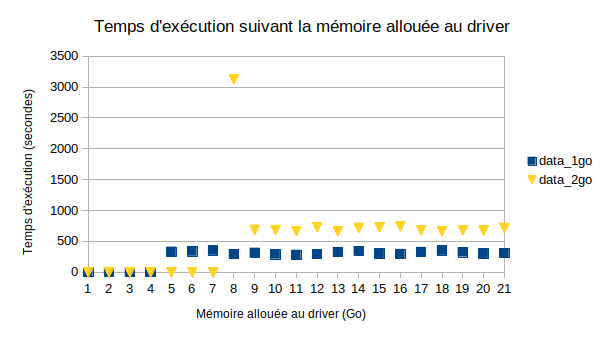
\includegraphics[width=1\linewidth]{illustrations/variant_driver_memory}
%	\caption{Mesure des temps d'exécution de l'application Spark selon différentes tailles de mémoire allouées au \textit{driver} et pour deux ensembles de données différentes}
%	\label{fig:variantdrivermemory}
%\end{figure}

%D'après la Figure 	\ref{fig:variantdrivermemory}, nous remarquons qu'à partir d'une taille mémoire allouée au driver, le temps écoulé durant l'exécution de l'application Spark est relativement stable. De plus, nous constatons qu'il faut prévoir une taille mémoire minimal pour assurer l'exécution de l'application Spark. Les tailles mémoire supérieures à cette valeur minimale affectent faiblement le temps d'exécution.  Cette valeur minimale dépend fortement de la quantité de données à analyser. Enfin, malgré que la machine sur laquelle nous lançons l'application Spark ne dispose que de $ 32 $ Go de RAM, le fait d'allouer au driver $ 35 $ Go, $ 40$ Go, $ 45 $ Go n'a pas généré une erreur lors de l'exécution.

\paragraph{Variant la taille des données analysées}~

Après avoir fixé la mémoire allouée au driver à $ 30 $. Plusieurs tests ont été réalisés en vue de mesurer le temps d'exécution en variant la tailles des échantillons de traceroutes. Le Tableau \ref{tab:spark-local} contient les temps d'exécution obtenus lors de 5 essais pour chaque échantillon de traceroutes. Les temps des essais et de la médiane des essais sont exprimés en secondes. 

\begin{table}[h]
	\resizebox{\textwidth}{!}{
	\begin{tabular}{cccccccccc}
\textbf{Période (début - fin)}	&\textbf{Taille de données (octets)}&	\textbf{Essai 1}	&\textbf{Essai 2}&\textbf{	Essai 3}&\textbf{	Essai 4}	&\textbf{Essai 5}&	\textbf{Médiane}&\textbf{	Ecart type}&	\textbf{Variance} \\ \hline
07/02/18 - 07/02/18&	$ 1,028,343,572 $&	$ 301 $&	$ 301 $&	$ 314 $	&$ 280 $	&$ 324 $	&$ 301 $&	$ 14.85 $	&$ 220.3 $ \\ \hline
07/02/18 - 08/02/18&	$ 2,055,167,238 $&	$ 722 $&	$ 645 $&	$ 597 $&	$ 655 $&	$ 603 $&	$ 645 $&	$ 50.24 $&	$ 2019.1 $ \\ \hline
07/02/18 - 09/02/18&	$ 3,083,779,157 $&	$ 1060 $&	$ 1015 $&	$ 984 $&	$ 978 $&	$ 978 $&	$ 984 $&	$ 35.37 $&	$ 1060.97 $ \\ \hline
07/02/18 - 10/02/18&	$ 4,113,776,434 $&	$ 1162 $&	$ 1103 $&	$ 1250 $&	$ 1265 $&	$ 1122 $&	$ 1162 $&	$ 73.73 $&	$ 4404.67 $ \\ \hline
07/02/18 - 11/02/18&	$ 5,143,831,662 $&	$ 1319 $&	$ 1243 $&	$ 1159 $	&$ 1184 $&	$ 1228 $&	$ 1228 $&	$ 61.64 $&	$ 3038.97 $ \\ \hline

	\end{tabular}
}
\caption{Temps d'exécution de l'analyse des délais avec Spark/Scala en mode local}
\label{tab:spark-local}
\end{table}

La Figure \ref{fig:spark-localmode} est une représentation graphique du temps médian obtenu en analysant les échantillons de traceroutes présentés dans le Tableau \ref{tab:spark-local}.

\begin{figure}[h]
	\centering
	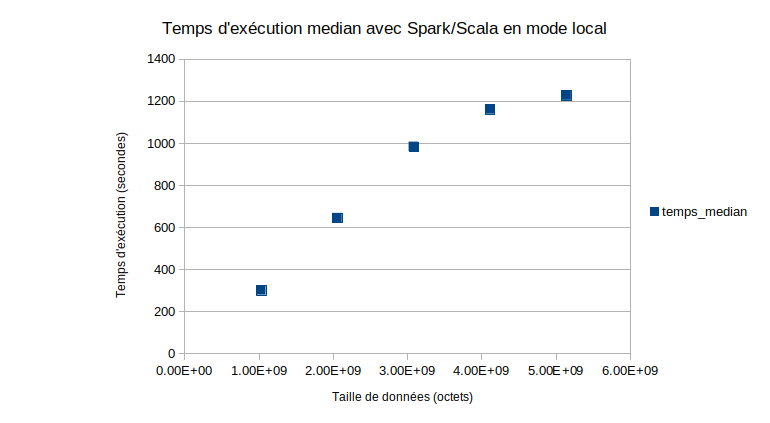
\includegraphics[width=\linewidth]{illustrations/spark-localmode2}
	\caption{Temps d'exécution médian avec l'implémentation  Spark/Scala en mode local}
	\label{fig:spark-localmode}
\end{figure}

\paragraph{Notes concernant le mode local}~

Le mode local d'exécution d'une application Spark est typiquement utilisé pour tester le code sur une petite quantité de données dans un environnement local. Cependant, ce mode  ne fournit pas les avantages de l'environnement distribué. C'est pourquoi nous avons évalué l'implémentation avec Spark/Scala sur un \textit{cluster} de machines. 

\subsection{Cluster Amazon EMR}

Nous évaluons le temps d'exécution obtenu lors du lancement de l'application de détection dans un \textit{cluster} créé au sein d'Amazon EMR. D'abord, nous  décrivons le déroulement de la création d'un \textit{cluster} dans Amazon EMR. Ensuite, nous mesurons le temps d'exécution de l'application de la détection sur différents \textit{clusters}. Ce temps inclut le temps nécessaire  pour chercher les traceroutes dans le compartiment d'Amazon S3, le temps nécessaire pour traiter ces données et  le temps pour créer le fichier résultat et le stocker dans un compartiment Amazon S3. Enfin, nous mesurons ce temps  aussi dans le cas d'un seul \textit{cluster}, choisi à l'avance, et en variant la taille  de données à analyser. Une brève présentation d'Amazon EMR est donnée dans la section \ref{emr-aws-presentation}.

\paragraph{Création d'un cluster EMR}~

La création d'un \textit{cluster} dans Amazon EMR destiné à une application Spark nécessite de  :
\begin{itemize}
	\item donner un nom au \textit{cluster};
	\item créer la configuration du \textit{cluster};
	\item définir le modèle du n\oe{}ud principal (\textit{master}) 
	\item choisir le nombre des n\oe{}uds de noyau  du \textit{cluster} et leur modèle;
	%\item paramétrer l'application Spark comme l'indication de la classe Main;
	\item spécifier les paramètres de l'application  (.jar) après avoir transférer l'archive vers  un compartiment Amazon S3;
	\item indiquer le chemin du compartiment Amazon S3 contenant  les données à analyser.
\end{itemize}

Nous avons énuméré quelques éléments demandés lors de la création et du déploiement d'une application Spark sur un \textit{cluster} Amazon EMR. Bien  qu'il existe d'autres paramètres qu'on peut ajuster. 

On distingue le temps nécessaire à la mise en place du \textit{cluster} et à la configuration du \textit{cluster} (\textit{Starting}). Une fois le \textit{cluster} est prêt, l'état du \textit{cluster} passe à (\textit{Waiting}).  A la soumission de l'application, le \textit{cluster} passe à l'état (Running). Suivant la configuration du \textit{cluster} de l'utilisateur, le \textit{cluster} peut s'éteindre dés la fin de l'exécution de l'application ou rester actif à l'écoute de nouvelles tâches. Toutefois, la dernière option peut produire des frais élevés.  


Ce que nous testons avec Amazon EMR sont les mêmes traitements que ceux dans le mode local. La première  différence est au niveau le nombre de machines qui forment le \textit{cluster}.   De plus, les traceroutes à analyser sans disponibles dans un compartiment Amazon S3, et les résultats de l'analyse sont sauvegardés dans un compartiment Amazon S3 (voir la Figure \ref{fig:sparktimingEMR}). 


\begin{figure}[H]
	\centering
	\captionsetup{justification=centering}
	\resizebox{\textwidth}{!}{
		% Graphic for TeX using PGF
% Title: /home/hayat/RipeAtlasTraceroutesAnalysis/2019/Rapport_Mai/illustrations/sparktimingEMR.dia
% Creator: Dia v0.97+git
% CreationDate: Wed May 29 20:11:55 2019
% For: hayat
% \usepackage{tikz}
% The following commands are not supported in PSTricks at present
% We define them conditionally, so when they are implemented,
% this pgf file will use them.
\ifx\du\undefined
  \newlength{\du}
\fi
\setlength{\du}{15\unitlength}
\begin{tikzpicture}[even odd rule]
\pgftransformxscale{1.000000}
\pgftransformyscale{-1.000000}
\definecolor{dialinecolor}{rgb}{0.000000, 0.000000, 0.000000}
\pgfsetstrokecolor{dialinecolor}
\pgfsetstrokeopacity{1.000000}
\definecolor{diafillcolor}{rgb}{1.000000, 1.000000, 1.000000}
\pgfsetfillcolor{diafillcolor}
\pgfsetfillopacity{1.000000}
\pgfsetlinewidth{0.100000\du}
\pgfsetdash{}{0pt}
\pgfsetbuttcap
\pgfsetmiterjoin
\pgfsetlinewidth{0.100000\du}
\pgfsetbuttcap
\pgfsetmiterjoin
\pgfsetdash{}{0pt}
\definecolor{diafillcolor}{rgb}{1.000000, 1.000000, 1.000000}
\pgfsetfillcolor{diafillcolor}
\pgfsetfillopacity{1.000000}
\definecolor{dialinecolor}{rgb}{0.000000, 0.000000, 0.000000}
\pgfsetstrokecolor{dialinecolor}
\pgfsetstrokeopacity{1.000000}
\pgfpathmoveto{\pgfpoint{29.698610\du}{4.301667\du}}
\pgfpathcurveto{\pgfpoint{30.208630\du}{4.026667\du}}{\pgfpoint{30.463640\du}{3.935000\du}}{\pgfpoint{30.973660\du}{3.935000\du}}
\pgfpathcurveto{\pgfpoint{31.483680\du}{3.935000\du}}{\pgfpoint{31.738690\du}{4.026667\du}}{\pgfpoint{32.248710\du}{4.301667\du}}
\pgfpathlineto{\pgfpoint{32.248710\du}{5.768333\du}}
\pgfpathcurveto{\pgfpoint{31.738690\du}{6.043333\du}}{\pgfpoint{31.483680\du}{6.135000\du}}{\pgfpoint{30.973660\du}{6.135000\du}}
\pgfpathcurveto{\pgfpoint{30.463640\du}{6.135000\du}}{\pgfpoint{30.208630\du}{6.043333\du}}{\pgfpoint{29.698610\du}{5.768333\du}}
\pgfpathlineto{\pgfpoint{29.698610\du}{4.301667\du}}
\pgfpathclose
\pgfusepath{fill,stroke}
\pgfsetbuttcap
\pgfsetmiterjoin
\pgfsetdash{}{0pt}
\definecolor{dialinecolor}{rgb}{0.000000, 0.000000, 0.000000}
\pgfsetstrokecolor{dialinecolor}
\pgfsetstrokeopacity{1.000000}
\pgfpathmoveto{\pgfpoint{29.698610\du}{4.301667\du}}
\pgfpathcurveto{\pgfpoint{30.208630\du}{4.576667\du}}{\pgfpoint{30.463640\du}{4.668333\du}}{\pgfpoint{30.973660\du}{4.668333\du}}
\pgfpathcurveto{\pgfpoint{31.483680\du}{4.668333\du}}{\pgfpoint{31.738690\du}{4.576667\du}}{\pgfpoint{32.248710\du}{4.301667\du}}
\pgfusepath{stroke}
% setfont left to latex
\definecolor{dialinecolor}{rgb}{0.000000, 0.000000, 0.000000}
\pgfsetstrokecolor{dialinecolor}
\pgfsetstrokeopacity{1.000000}
\definecolor{diafillcolor}{rgb}{0.000000, 0.000000, 0.000000}
\pgfsetfillcolor{diafillcolor}
\pgfsetfillopacity{1.000000}
\node[anchor=base,inner sep=0pt, outer sep=0pt,color=dialinecolor] at (30.973660\du,5.418333\du){};
% setfont left to latex
\definecolor{dialinecolor}{rgb}{0.000000, 0.000000, 0.000000}
\pgfsetstrokecolor{dialinecolor}
\pgfsetstrokeopacity{1.000000}
\definecolor{diafillcolor}{rgb}{0.000000, 0.000000, 0.000000}
\pgfsetfillcolor{diafillcolor}
\pgfsetfillopacity{1.000000}
\node[anchor=base west,inner sep=0pt,outer sep=0pt,color=dialinecolor] at (29.298610\du,3.335000\du){Amazon S3};
\pgfsetlinewidth{0.100000\du}
\pgfsetdash{{\pgflinewidth}{0.200000\du}}{0cm}
\pgfsetbuttcap
{
\definecolor{diafillcolor}{rgb}{0.000000, 0.000000, 0.000000}
\pgfsetfillcolor{diafillcolor}
\pgfsetfillopacity{1.000000}
% was here!!!
\pgfsetarrowsend{stealth}
\definecolor{dialinecolor}{rgb}{0.000000, 0.000000, 0.000000}
\pgfsetstrokecolor{dialinecolor}
\pgfsetstrokeopacity{1.000000}
\draw (21.950063\du,12.085000\du)--(57.900063\du,12.140000\du);
}
\pgfsetlinewidth{0.000000\du}
\pgfsetdash{}{0pt}
\pgfsetmiterjoin
{\pgfsetcornersarced{\pgfpoint{0.000000\du}{0.000000\du}}\definecolor{diafillcolor}{rgb}{1.000000, 1.000000, 1.000000}
\pgfsetfillcolor{diafillcolor}
\pgfsetfillopacity{1.000000}
\fill (34.362410\du,0.235000\du)--(34.362410\du,2.835000\du)--(43.432410\du,2.835000\du)--(43.432410\du,0.235000\du)--cycle;
}{\pgfsetcornersarced{\pgfpoint{0.000000\du}{0.000000\du}}\definecolor{dialinecolor}{rgb}{0.000000, 0.000000, 0.000000}
\pgfsetstrokecolor{dialinecolor}
\pgfsetstrokeopacity{1.000000}
\draw (34.362410\du,0.235000\du)--(34.362410\du,2.835000\du)--(43.432410\du,2.835000\du)--(43.432410\du,0.235000\du)--cycle;
}% setfont left to latex
\definecolor{dialinecolor}{rgb}{0.000000, 0.000000, 0.000000}
\pgfsetstrokecolor{dialinecolor}
\pgfsetstrokeopacity{1.000000}
\definecolor{diafillcolor}{rgb}{0.000000, 0.000000, 0.000000}
\pgfsetfillcolor{diafillcolor}
\pgfsetfillopacity{1.000000}
\node[anchor=base,inner sep=0pt, outer sep=0pt,color=dialinecolor] at (38.897410\du,1.330000\du){Analyser les traceroutes };
% setfont left to latex
\definecolor{dialinecolor}{rgb}{0.000000, 0.000000, 0.000000}
\pgfsetstrokecolor{dialinecolor}
\pgfsetstrokeopacity{1.000000}
\definecolor{diafillcolor}{rgb}{0.000000, 0.000000, 0.000000}
\pgfsetfillcolor{diafillcolor}
\pgfsetfillopacity{1.000000}
\node[anchor=base,inner sep=0pt, outer sep=0pt,color=dialinecolor] at (38.897410\du,2.130000\du){(Fontugne et al.)};
\pgfsetlinewidth{0.100000\du}
\pgfsetdash{}{0pt}
\pgfsetmiterjoin
{\pgfsetcornersarced{\pgfpoint{0.000000\du}{0.000000\du}}\definecolor{diafillcolor}{rgb}{1.000000, 1.000000, 1.000000}
\pgfsetfillcolor{diafillcolor}
\pgfsetfillopacity{1.000000}
\fill (46.002460\du,3.035000\du)--(46.002460\du,5.933955\du)--(52.095060\du,5.933955\du)--(52.095060\du,3.035000\du)--cycle;
}{\pgfsetcornersarced{\pgfpoint{0.000000\du}{0.000000\du}}\definecolor{dialinecolor}{rgb}{0.000000, 0.000000, 0.000000}
\pgfsetstrokecolor{dialinecolor}
\pgfsetstrokeopacity{1.000000}
\draw (46.002460\du,3.035000\du)--(46.002460\du,5.933955\du)--(52.095060\du,5.933955\du)--(52.095060\du,3.035000\du)--cycle;
}% setfont left to latex
\definecolor{dialinecolor}{rgb}{0.000000, 0.000000, 0.000000}
\pgfsetstrokecolor{dialinecolor}
\pgfsetstrokeopacity{1.000000}
\definecolor{diafillcolor}{rgb}{0.000000, 0.000000, 0.000000}
\pgfsetfillcolor{diafillcolor}
\pgfsetfillopacity{1.000000}
\node[anchor=base,inner sep=0pt, outer sep=0pt,color=dialinecolor] at (49.048760\du,4.279477\du){sauvegarder };
% setfont left to latex
\definecolor{dialinecolor}{rgb}{0.000000, 0.000000, 0.000000}
\pgfsetstrokecolor{dialinecolor}
\pgfsetstrokeopacity{1.000000}
\definecolor{diafillcolor}{rgb}{0.000000, 0.000000, 0.000000}
\pgfsetfillcolor{diafillcolor}
\pgfsetfillopacity{1.000000}
\node[anchor=base,inner sep=0pt, outer sep=0pt,color=dialinecolor] at (49.048760\du,5.079477\du){les résultats};
\pgfsetlinewidth{0.100000\du}
\pgfsetdash{}{0pt}
\pgfsetbuttcap
\pgfsetmiterjoin
\pgfsetlinewidth{0.100000\du}
\pgfsetbuttcap
\pgfsetmiterjoin
\pgfsetdash{}{0pt}
\definecolor{diafillcolor}{rgb}{1.000000, 1.000000, 1.000000}
\pgfsetfillcolor{diafillcolor}
\pgfsetfillopacity{1.000000}
\definecolor{dialinecolor}{rgb}{0.000000, 0.000000, 0.000000}
\pgfsetstrokecolor{dialinecolor}
\pgfsetstrokeopacity{1.000000}
\pgfpathmoveto{\pgfpoint{54.395100\du}{4.251667\du}}
\pgfpathcurveto{\pgfpoint{54.905120\du}{3.976667\du}}{\pgfpoint{55.160130\du}{3.885000\du}}{\pgfpoint{55.670150\du}{3.885000\du}}
\pgfpathcurveto{\pgfpoint{56.180170\du}{3.885000\du}}{\pgfpoint{56.435180\du}{3.976667\du}}{\pgfpoint{56.945200\du}{4.251667\du}}
\pgfpathlineto{\pgfpoint{56.945200\du}{5.718333\du}}
\pgfpathcurveto{\pgfpoint{56.435180\du}{5.993333\du}}{\pgfpoint{56.180170\du}{6.085000\du}}{\pgfpoint{55.670150\du}{6.085000\du}}
\pgfpathcurveto{\pgfpoint{55.160130\du}{6.085000\du}}{\pgfpoint{54.905120\du}{5.993333\du}}{\pgfpoint{54.395100\du}{5.718333\du}}
\pgfpathlineto{\pgfpoint{54.395100\du}{4.251667\du}}
\pgfpathclose
\pgfusepath{fill,stroke}
\pgfsetbuttcap
\pgfsetmiterjoin
\pgfsetdash{}{0pt}
\definecolor{dialinecolor}{rgb}{0.000000, 0.000000, 0.000000}
\pgfsetstrokecolor{dialinecolor}
\pgfsetstrokeopacity{1.000000}
\pgfpathmoveto{\pgfpoint{54.395100\du}{4.251667\du}}
\pgfpathcurveto{\pgfpoint{54.905120\du}{4.526667\du}}{\pgfpoint{55.160130\du}{4.618333\du}}{\pgfpoint{55.670150\du}{4.618333\du}}
\pgfpathcurveto{\pgfpoint{56.180170\du}{4.618333\du}}{\pgfpoint{56.435180\du}{4.526667\du}}{\pgfpoint{56.945200\du}{4.251667\du}}
\pgfusepath{stroke}
% setfont left to latex
\definecolor{dialinecolor}{rgb}{0.000000, 0.000000, 0.000000}
\pgfsetstrokecolor{dialinecolor}
\pgfsetstrokeopacity{1.000000}
\definecolor{diafillcolor}{rgb}{0.000000, 0.000000, 0.000000}
\pgfsetfillcolor{diafillcolor}
\pgfsetfillopacity{1.000000}
\node[anchor=base,inner sep=0pt, outer sep=0pt,color=dialinecolor] at (55.670150\du,5.368333\du){};
% setfont left to latex
\definecolor{dialinecolor}{rgb}{0.000000, 0.000000, 0.000000}
\pgfsetstrokecolor{dialinecolor}
\pgfsetstrokeopacity{1.000000}
\definecolor{diafillcolor}{rgb}{0.000000, 0.000000, 0.000000}
\pgfsetfillcolor{diafillcolor}
\pgfsetfillopacity{1.000000}
\node[anchor=base west,inner sep=0pt,outer sep=0pt,color=dialinecolor] at (53.995100\du,3.285000\du){Amazon S3};
\pgfsetlinewidth{0.100000\du}
\pgfsetdash{}{0pt}
\pgfsetbuttcap
{
\definecolor{diafillcolor}{rgb}{0.000000, 0.000000, 0.000000}
\pgfsetfillcolor{diafillcolor}
\pgfsetfillopacity{1.000000}
% was here!!!
\pgfsetarrowsend{to}
\definecolor{dialinecolor}{rgb}{0.000000, 0.000000, 0.000000}
\pgfsetstrokecolor{dialinecolor}
\pgfsetstrokeopacity{1.000000}
\pgfpathmoveto{\pgfpoint{51.950010\du}{6.349911\du}}
\pgfpatharc{135}{44}{1.917451\du and 1.917451\du}
\pgfusepath{stroke}
}
\pgfsetlinewidth{0.100000\du}
\pgfsetdash{}{0pt}
\pgfsetbuttcap
{
\definecolor{diafillcolor}{rgb}{0.000000, 0.000000, 0.000000}
\pgfsetfillcolor{diafillcolor}
\pgfsetfillopacity{1.000000}
% was here!!!
\pgfsetarrowsend{to}
\definecolor{dialinecolor}{rgb}{0.000000, 0.000000, 0.000000}
\pgfsetstrokecolor{dialinecolor}
\pgfsetstrokeopacity{1.000000}
\pgfpathmoveto{\pgfpoint{45.450064\du}{4.734995\du}}
\pgfpatharc{373}{251}{1.231323\du and 1.231323\du}
\pgfusepath{stroke}
}
\pgfsetlinewidth{0.100000\du}
\pgfsetdash{}{0pt}
\pgfsetbuttcap
{
\definecolor{diafillcolor}{rgb}{0.000000, 0.000000, 0.000000}
\pgfsetfillcolor{diafillcolor}
\pgfsetfillopacity{1.000000}
% was here!!!
\pgfsetarrowsend{to}
\definecolor{dialinecolor}{rgb}{0.000000, 0.000000, 0.000000}
\pgfsetstrokecolor{dialinecolor}
\pgfsetstrokeopacity{1.000000}
\pgfpathmoveto{\pgfpoint{32.699947\du}{4.334966\du}}
\pgfpatharc{107}{13}{1.632070\du and 1.632070\du}
\pgfusepath{stroke}
}
\pgfsetlinewidth{0.100000\du}
\pgfsetdash{}{0pt}
\pgfsetbuttcap
{
\definecolor{diafillcolor}{rgb}{0.000000, 0.000000, 0.000000}
\pgfsetfillcolor{diafillcolor}
\pgfsetfillopacity{1.000000}
% was here!!!
\pgfsetarrowsend{to}
\definecolor{dialinecolor}{rgb}{0.000000, 0.000000, 0.000000}
\pgfsetstrokecolor{dialinecolor}
\pgfsetstrokeopacity{1.000000}
\pgfpathmoveto{\pgfpoint{27.036079\du}{6.330367\du}}
\pgfpatharc{135}{44}{1.917451\du and 1.917451\du}
\pgfusepath{stroke}
}
\pgfsetlinewidth{0.100000\du}
\pgfsetdash{}{0pt}
\pgfsetmiterjoin
{\pgfsetcornersarced{\pgfpoint{0.000000\du}{0.000000\du}}\definecolor{diafillcolor}{rgb}{1.000000, 1.000000, 1.000000}
\pgfsetfillcolor{diafillcolor}
\pgfsetfillopacity{1.000000}
\fill (22.125063\du,3.230000\du)--(22.125063\du,6.145000\du)--(26.976073\du,6.145000\du)--(26.976073\du,3.230000\du)--cycle;
}{\pgfsetcornersarced{\pgfpoint{0.000000\du}{0.000000\du}}\definecolor{dialinecolor}{rgb}{0.000000, 0.000000, 0.000000}
\pgfsetstrokecolor{dialinecolor}
\pgfsetstrokeopacity{1.000000}
\draw (22.125063\du,3.230000\du)--(22.125063\du,6.145000\du)--(26.976073\du,6.145000\du)--(26.976073\du,3.230000\du)--cycle;
}% setfont left to latex
\definecolor{dialinecolor}{rgb}{0.000000, 0.000000, 0.000000}
\pgfsetstrokecolor{dialinecolor}
\pgfsetstrokeopacity{1.000000}
\definecolor{diafillcolor}{rgb}{0.000000, 0.000000, 0.000000}
\pgfsetfillcolor{diafillcolor}
\pgfsetfillopacity{1.000000}
\node[anchor=base,inner sep=0pt, outer sep=0pt,color=dialinecolor] at (24.550568\du,4.482500\du){Paramètrer};
% setfont left to latex
\definecolor{dialinecolor}{rgb}{0.000000, 0.000000, 0.000000}
\pgfsetstrokecolor{dialinecolor}
\pgfsetstrokeopacity{1.000000}
\definecolor{diafillcolor}{rgb}{0.000000, 0.000000, 0.000000}
\pgfsetfillcolor{diafillcolor}
\pgfsetfillopacity{1.000000}
\node[anchor=base,inner sep=0pt, outer sep=0pt,color=dialinecolor] at (24.550568\du,5.282500\du){l'analyse};
\pgfsetlinewidth{0.100000\du}
\pgfsetdash{}{0pt}
\pgfsetbuttcap
\pgfsetmiterjoin
\pgfsetlinewidth{0.001000\du}
\pgfsetbuttcap
\pgfsetmiterjoin
\pgfsetdash{}{0pt}
\definecolor{diafillcolor}{rgb}{0.717647, 0.717647, 0.615686}
\pgfsetfillcolor{diafillcolor}
\pgfsetfillopacity{1.000000}
\pgfpathmoveto{\pgfpoint{36.597434\du}{5.833245\du}}
\pgfpathlineto{\pgfpoint{37.779850\du}{5.833245\du}}
\pgfpathlineto{\pgfpoint{37.779850\du}{6.051770\du}}
\pgfpathlineto{\pgfpoint{36.597434\du}{6.051770\du}}
\pgfpathlineto{\pgfpoint{36.597434\du}{5.833245\du}}
\pgfpathclose
\pgfusepath{fill}
\pgfsetbuttcap
\pgfsetmiterjoin
\pgfsetdash{}{0pt}
\definecolor{dialinecolor}{rgb}{0.286275, 0.286275, 0.211765}
\pgfsetstrokecolor{dialinecolor}
\pgfsetstrokeopacity{1.000000}
\pgfpathmoveto{\pgfpoint{36.597434\du}{5.833245\du}}
\pgfpathlineto{\pgfpoint{37.779850\du}{5.833245\du}}
\pgfpathlineto{\pgfpoint{37.779850\du}{6.051770\du}}
\pgfpathlineto{\pgfpoint{36.597434\du}{6.051770\du}}
\pgfpathlineto{\pgfpoint{36.597434\du}{5.833245\du}}
\pgfusepath{stroke}
\pgfsetbuttcap
\pgfsetmiterjoin
\pgfsetdash{}{0pt}
\definecolor{diafillcolor}{rgb}{0.788235, 0.788235, 0.713726}
\pgfsetfillcolor{diafillcolor}
\pgfsetfillopacity{1.000000}
\pgfpathmoveto{\pgfpoint{36.597434\du}{5.833245\du}}
\pgfpathlineto{\pgfpoint{36.722811\du}{5.714389\du}}
\pgfpathlineto{\pgfpoint{37.905227\du}{5.714389\du}}
\pgfpathlineto{\pgfpoint{37.779850\du}{5.833245\du}}
\pgfpathlineto{\pgfpoint{36.597434\du}{5.833245\du}}
\pgfpathclose
\pgfusepath{fill}
\pgfsetbuttcap
\pgfsetmiterjoin
\pgfsetdash{}{0pt}
\definecolor{dialinecolor}{rgb}{0.286275, 0.286275, 0.211765}
\pgfsetstrokecolor{dialinecolor}
\pgfsetstrokeopacity{1.000000}
\pgfpathmoveto{\pgfpoint{36.597434\du}{5.833245\du}}
\pgfpathlineto{\pgfpoint{36.722811\du}{5.714389\du}}
\pgfpathlineto{\pgfpoint{37.905227\du}{5.714389\du}}
\pgfpathlineto{\pgfpoint{37.779850\du}{5.833245\du}}
\pgfpathlineto{\pgfpoint{36.597434\du}{5.833245\du}}
\pgfusepath{stroke}
\pgfsetlinewidth{0.106000\du}
\pgfsetbuttcap
\pgfsetmiterjoin
\pgfsetdash{}{0pt}
\definecolor{dialinecolor}{rgb}{0.000000, 0.000000, 0.000000}
\pgfsetstrokecolor{dialinecolor}
\pgfsetstrokeopacity{1.000000}
\pgfpathmoveto{\pgfpoint{37.713715\du}{5.932727\du}}
\pgfpathlineto{\pgfpoint{37.429988\du}{5.932727\du}}
\pgfusepath{stroke}
\pgfsetlinewidth{0.001000\du}
\pgfsetbuttcap
\pgfsetmiterjoin
\pgfsetdash{}{0pt}
\definecolor{diafillcolor}{rgb}{0.478431, 0.478431, 0.352941}
\pgfsetfillcolor{diafillcolor}
\pgfsetfillopacity{1.000000}
\pgfpathmoveto{\pgfpoint{37.779850\du}{6.051770\du}}
\pgfpathlineto{\pgfpoint{37.905227\du}{5.926020\du}}
\pgfpathlineto{\pgfpoint{37.905227\du}{5.714389\du}}
\pgfpathlineto{\pgfpoint{37.779850\du}{5.833245\du}}
\pgfpathlineto{\pgfpoint{37.779850\du}{6.051770\du}}
\pgfpathclose
\pgfusepath{fill}
\pgfsetbuttcap
\pgfsetmiterjoin
\pgfsetdash{}{0pt}
\definecolor{dialinecolor}{rgb}{0.286275, 0.286275, 0.211765}
\pgfsetstrokecolor{dialinecolor}
\pgfsetstrokeopacity{1.000000}
\pgfpathmoveto{\pgfpoint{37.779850\du}{6.051770\du}}
\pgfpathlineto{\pgfpoint{37.905227\du}{5.926020\du}}
\pgfpathlineto{\pgfpoint{37.905227\du}{5.714389\du}}
\pgfpathlineto{\pgfpoint{37.779850\du}{5.833245\du}}
\pgfpathlineto{\pgfpoint{37.779850\du}{6.051770\du}}
\pgfusepath{stroke}
\pgfsetbuttcap
\pgfsetmiterjoin
\pgfsetdash{}{0pt}
\definecolor{diafillcolor}{rgb}{0.788235, 0.788235, 0.713726}
\pgfsetfillcolor{diafillcolor}
\pgfsetfillopacity{1.000000}
\pgfpathmoveto{\pgfpoint{36.604141\du}{6.190373\du}}
\pgfpathlineto{\pgfpoint{36.736038\du}{6.025129\du}}
\pgfpathlineto{\pgfpoint{37.647767\du}{6.025129\du}}
\pgfpathlineto{\pgfpoint{37.515870\du}{6.190373\du}}
\pgfpathlineto{\pgfpoint{36.604141\du}{6.190373\du}}
\pgfpathclose
\pgfusepath{fill}
\pgfsetbuttcap
\pgfsetmiterjoin
\pgfsetdash{}{0pt}
\definecolor{dialinecolor}{rgb}{0.286275, 0.286275, 0.211765}
\pgfsetstrokecolor{dialinecolor}
\pgfsetstrokeopacity{1.000000}
\pgfpathmoveto{\pgfpoint{36.604141\du}{6.190373\du}}
\pgfpathlineto{\pgfpoint{36.736038\du}{6.025129\du}}
\pgfpathlineto{\pgfpoint{37.647767\du}{6.025129\du}}
\pgfpathlineto{\pgfpoint{37.515870\du}{6.190373\du}}
\pgfpathlineto{\pgfpoint{36.604141\du}{6.190373\du}}
\pgfusepath{stroke}
\pgfsetbuttcap
\pgfsetmiterjoin
\pgfsetdash{}{0pt}
\definecolor{diafillcolor}{rgb}{0.478431, 0.478431, 0.352941}
\pgfsetfillcolor{diafillcolor}
\pgfsetfillopacity{1.000000}
\pgfpathmoveto{\pgfpoint{37.515870\du}{6.223348\du}}
\pgfpathlineto{\pgfpoint{37.647767\du}{6.084744\du}}
\pgfpathlineto{\pgfpoint{37.647767\du}{6.025129\du}}
\pgfpathlineto{\pgfpoint{37.515870\du}{6.190373\du}}
\pgfpathlineto{\pgfpoint{37.515870\du}{6.223348\du}}
\pgfpathclose
\pgfusepath{fill}
\pgfsetbuttcap
\pgfsetmiterjoin
\pgfsetdash{}{0pt}
\definecolor{dialinecolor}{rgb}{0.286275, 0.286275, 0.211765}
\pgfsetstrokecolor{dialinecolor}
\pgfsetstrokeopacity{1.000000}
\pgfpathmoveto{\pgfpoint{37.515870\du}{6.223348\du}}
\pgfpathlineto{\pgfpoint{37.647767\du}{6.084744\du}}
\pgfpathlineto{\pgfpoint{37.647767\du}{6.025129\du}}
\pgfpathlineto{\pgfpoint{37.515870\du}{6.190373\du}}
\pgfpathlineto{\pgfpoint{37.515870\du}{6.223348\du}}
\pgfusepath{stroke}
\pgfsetbuttcap
\pgfsetmiterjoin
\pgfsetdash{}{0pt}
\definecolor{diafillcolor}{rgb}{0.717647, 0.717647, 0.615686}
\pgfsetfillcolor{diafillcolor}
\pgfsetfillopacity{1.000000}
\pgfpathmoveto{\pgfpoint{36.604141\du}{6.190373\du}}
\pgfpathlineto{\pgfpoint{37.515870\du}{6.190373\du}}
\pgfpathlineto{\pgfpoint{37.515870\du}{6.223348\du}}
\pgfpathlineto{\pgfpoint{36.604141\du}{6.223348\du}}
\pgfpathlineto{\pgfpoint{36.604141\du}{6.190373\du}}
\pgfpathclose
\pgfusepath{fill}
\pgfsetbuttcap
\pgfsetmiterjoin
\pgfsetdash{}{0pt}
\definecolor{dialinecolor}{rgb}{0.286275, 0.286275, 0.211765}
\pgfsetstrokecolor{dialinecolor}
\pgfsetstrokeopacity{1.000000}
\pgfpathmoveto{\pgfpoint{36.604141\du}{6.190373\du}}
\pgfpathlineto{\pgfpoint{37.515870\du}{6.190373\du}}
\pgfpathlineto{\pgfpoint{37.515870\du}{6.223348\du}}
\pgfpathlineto{\pgfpoint{36.604141\du}{6.223348\du}}
\pgfpathlineto{\pgfpoint{36.604141\du}{6.190373\du}}
\pgfusepath{stroke}
\pgfsetbuttcap
\pgfsetmiterjoin
\pgfsetdash{}{0pt}
\definecolor{diafillcolor}{rgb}{0.000000, 0.000000, 0.000000}
\pgfsetfillcolor{diafillcolor}
\pgfsetfillopacity{1.000000}
\pgfpathmoveto{\pgfpoint{36.775719\du}{5.806978\du}}
\pgfpathlineto{\pgfpoint{36.875014\du}{5.714389\du}}
\pgfpathlineto{\pgfpoint{37.713715\du}{5.714389\du}}
\pgfpathlineto{\pgfpoint{37.621499\du}{5.806978\du}}
\pgfpathlineto{\pgfpoint{36.775719\du}{5.806978\du}}
\pgfpathclose
\pgfusepath{fill}
\pgfsetbuttcap
\pgfsetmiterjoin
\pgfsetdash{}{0pt}
\definecolor{dialinecolor}{rgb}{0.000000, 0.000000, 0.000000}
\pgfsetstrokecolor{dialinecolor}
\pgfsetstrokeopacity{1.000000}
\pgfpathmoveto{\pgfpoint{36.775719\du}{5.806978\du}}
\pgfpathlineto{\pgfpoint{36.875014\du}{5.714389\du}}
\pgfpathlineto{\pgfpoint{37.713715\du}{5.714389\du}}
\pgfpathlineto{\pgfpoint{37.621499\du}{5.806978\du}}
\pgfpathlineto{\pgfpoint{36.775719\du}{5.806978\du}}
\pgfusepath{stroke}
\pgfsetbuttcap
\pgfsetmiterjoin
\pgfsetdash{}{0pt}
\definecolor{diafillcolor}{rgb}{0.788235, 0.788235, 0.713726}
\pgfsetfillcolor{diafillcolor}
\pgfsetfillopacity{1.000000}
\pgfpathmoveto{\pgfpoint{36.769012\du}{5.125882\du}}
\pgfpathlineto{\pgfpoint{36.861787\du}{5.040000\du}}
\pgfpathlineto{\pgfpoint{37.700861\du}{5.040000\du}}
\pgfpathlineto{\pgfpoint{37.608086\du}{5.125882\du}}
\pgfpathlineto{\pgfpoint{36.769012\du}{5.125882\du}}
\pgfpathclose
\pgfusepath{fill}
\pgfsetbuttcap
\pgfsetmiterjoin
\pgfsetdash{}{0pt}
\definecolor{dialinecolor}{rgb}{0.286275, 0.286275, 0.211765}
\pgfsetstrokecolor{dialinecolor}
\pgfsetstrokeopacity{1.000000}
\pgfpathmoveto{\pgfpoint{36.769012\du}{5.125882\du}}
\pgfpathlineto{\pgfpoint{36.861787\du}{5.040000\du}}
\pgfpathlineto{\pgfpoint{37.700861\du}{5.040000\du}}
\pgfpathlineto{\pgfpoint{37.608086\du}{5.125882\du}}
\pgfpathlineto{\pgfpoint{36.769012\du}{5.125882\du}}
\pgfusepath{stroke}
\pgfsetbuttcap
\pgfsetmiterjoin
\pgfsetdash{}{0pt}
\definecolor{diafillcolor}{rgb}{0.717647, 0.717647, 0.615686}
\pgfsetfillcolor{diafillcolor}
\pgfsetfillopacity{1.000000}
\pgfpathmoveto{\pgfpoint{36.769012\du}{5.125882\du}}
\pgfpathlineto{\pgfpoint{37.614792\du}{5.125882\du}}
\pgfpathlineto{\pgfpoint{37.614792\du}{5.793564\du}}
\pgfpathlineto{\pgfpoint{36.769012\du}{5.793564\du}}
\pgfpathlineto{\pgfpoint{36.769012\du}{5.125882\du}}
\pgfpathclose
\pgfusepath{fill}
\pgfsetbuttcap
\pgfsetmiterjoin
\pgfsetdash{}{0pt}
\definecolor{dialinecolor}{rgb}{0.286275, 0.286275, 0.211765}
\pgfsetstrokecolor{dialinecolor}
\pgfsetstrokeopacity{1.000000}
\pgfpathmoveto{\pgfpoint{36.769012\du}{5.125882\du}}
\pgfpathlineto{\pgfpoint{37.614420\du}{5.125882\du}}
\pgfpathlineto{\pgfpoint{37.614420\du}{5.793378\du}}
\pgfpathlineto{\pgfpoint{36.769012\du}{5.793378\du}}
\pgfpathlineto{\pgfpoint{36.769012\du}{5.125882\du}}
\pgfusepath{stroke}
\pgfsetbuttcap
\pgfsetmiterjoin
\pgfsetdash{}{0pt}
\definecolor{diafillcolor}{rgb}{1.000000, 1.000000, 1.000000}
\pgfsetfillcolor{diafillcolor}
\pgfsetfillopacity{1.000000}
\pgfpathmoveto{\pgfpoint{36.841667\du}{5.211578\du}}
\pgfpathlineto{\pgfpoint{37.541951\du}{5.211578\du}}
\pgfpathlineto{\pgfpoint{37.541951\du}{5.727430\du}}
\pgfpathlineto{\pgfpoint{36.841667\du}{5.727430\du}}
\pgfpathlineto{\pgfpoint{36.841667\du}{5.211578\du}}
\pgfpathclose
\pgfusepath{fill}
\pgfsetbuttcap
\pgfsetmiterjoin
\pgfsetdash{}{0pt}
\definecolor{dialinecolor}{rgb}{0.286275, 0.286275, 0.211765}
\pgfsetstrokecolor{dialinecolor}
\pgfsetstrokeopacity{1.000000}
\pgfpathmoveto{\pgfpoint{36.841667\du}{5.211578\du}}
\pgfpathlineto{\pgfpoint{37.541951\du}{5.211578\du}}
\pgfpathlineto{\pgfpoint{37.541951\du}{5.727243\du}}
\pgfpathlineto{\pgfpoint{36.841667\du}{5.727243\du}}
\pgfpathlineto{\pgfpoint{36.841667\du}{5.211578\du}}
\pgfusepath{stroke}
\pgfsetbuttcap
\pgfsetmiterjoin
\pgfsetdash{}{0pt}
\definecolor{diafillcolor}{rgb}{0.478431, 0.478431, 0.352941}
\pgfsetfillcolor{diafillcolor}
\pgfsetfillopacity{1.000000}
\pgfpathmoveto{\pgfpoint{37.608086\du}{5.787230\du}}
\pgfpathlineto{\pgfpoint{37.700861\du}{5.694642\du}}
\pgfpathlineto{\pgfpoint{37.700861\du}{5.040000\du}}
\pgfpathlineto{\pgfpoint{37.608086\du}{5.125882\du}}
\pgfpathlineto{\pgfpoint{37.608086\du}{5.787230\du}}
\pgfpathclose
\pgfusepath{fill}
\pgfsetbuttcap
\pgfsetmiterjoin
\pgfsetdash{}{0pt}
\definecolor{dialinecolor}{rgb}{0.286275, 0.286275, 0.211765}
\pgfsetstrokecolor{dialinecolor}
\pgfsetstrokeopacity{1.000000}
\pgfpathmoveto{\pgfpoint{37.608086\du}{5.787230\du}}
\pgfpathlineto{\pgfpoint{37.700861\du}{5.694642\du}}
\pgfpathlineto{\pgfpoint{37.700861\du}{5.040000\du}}
\pgfpathlineto{\pgfpoint{37.608086\du}{5.125882\du}}
\pgfpathlineto{\pgfpoint{37.608086\du}{5.787230\du}}
\pgfusepath{stroke}
\pgfsetlinewidth{0.100000\du}
\pgfsetdash{}{0pt}
\pgfsetbuttcap
\pgfsetmiterjoin
\pgfsetlinewidth{0.001000\du}
\pgfsetbuttcap
\pgfsetmiterjoin
\pgfsetdash{}{0pt}
\definecolor{diafillcolor}{rgb}{0.717647, 0.717647, 0.615686}
\pgfsetfillcolor{diafillcolor}
\pgfsetfillopacity{1.000000}
\pgfpathmoveto{\pgfpoint{39.577571\du}{5.825534\du}}
\pgfpathlineto{\pgfpoint{40.759988\du}{5.825534\du}}
\pgfpathlineto{\pgfpoint{40.759988\du}{6.044058\du}}
\pgfpathlineto{\pgfpoint{39.577571\du}{6.044058\du}}
\pgfpathlineto{\pgfpoint{39.577571\du}{5.825534\du}}
\pgfpathclose
\pgfusepath{fill}
\pgfsetbuttcap
\pgfsetmiterjoin
\pgfsetdash{}{0pt}
\definecolor{dialinecolor}{rgb}{0.286275, 0.286275, 0.211765}
\pgfsetstrokecolor{dialinecolor}
\pgfsetstrokeopacity{1.000000}
\pgfpathmoveto{\pgfpoint{39.577571\du}{5.825534\du}}
\pgfpathlineto{\pgfpoint{40.759988\du}{5.825534\du}}
\pgfpathlineto{\pgfpoint{40.759988\du}{6.044058\du}}
\pgfpathlineto{\pgfpoint{39.577571\du}{6.044058\du}}
\pgfpathlineto{\pgfpoint{39.577571\du}{5.825534\du}}
\pgfusepath{stroke}
\pgfsetbuttcap
\pgfsetmiterjoin
\pgfsetdash{}{0pt}
\definecolor{diafillcolor}{rgb}{0.788235, 0.788235, 0.713726}
\pgfsetfillcolor{diafillcolor}
\pgfsetfillopacity{1.000000}
\pgfpathmoveto{\pgfpoint{39.577571\du}{5.825534\du}}
\pgfpathlineto{\pgfpoint{39.702948\du}{5.706677\du}}
\pgfpathlineto{\pgfpoint{40.885364\du}{5.706677\du}}
\pgfpathlineto{\pgfpoint{40.759988\du}{5.825534\du}}
\pgfpathlineto{\pgfpoint{39.577571\du}{5.825534\du}}
\pgfpathclose
\pgfusepath{fill}
\pgfsetbuttcap
\pgfsetmiterjoin
\pgfsetdash{}{0pt}
\definecolor{dialinecolor}{rgb}{0.286275, 0.286275, 0.211765}
\pgfsetstrokecolor{dialinecolor}
\pgfsetstrokeopacity{1.000000}
\pgfpathmoveto{\pgfpoint{39.577571\du}{5.825534\du}}
\pgfpathlineto{\pgfpoint{39.702948\du}{5.706677\du}}
\pgfpathlineto{\pgfpoint{40.885364\du}{5.706677\du}}
\pgfpathlineto{\pgfpoint{40.759988\du}{5.825534\du}}
\pgfpathlineto{\pgfpoint{39.577571\du}{5.825534\du}}
\pgfusepath{stroke}
\pgfsetlinewidth{0.106000\du}
\pgfsetbuttcap
\pgfsetmiterjoin
\pgfsetdash{}{0pt}
\definecolor{dialinecolor}{rgb}{0.000000, 0.000000, 0.000000}
\pgfsetstrokecolor{dialinecolor}
\pgfsetstrokeopacity{1.000000}
\pgfpathmoveto{\pgfpoint{40.693853\du}{5.925015\du}}
\pgfpathlineto{\pgfpoint{40.410125\du}{5.925015\du}}
\pgfusepath{stroke}
\pgfsetlinewidth{0.001000\du}
\pgfsetbuttcap
\pgfsetmiterjoin
\pgfsetdash{}{0pt}
\definecolor{diafillcolor}{rgb}{0.478431, 0.478431, 0.352941}
\pgfsetfillcolor{diafillcolor}
\pgfsetfillopacity{1.000000}
\pgfpathmoveto{\pgfpoint{40.759988\du}{6.044058\du}}
\pgfpathlineto{\pgfpoint{40.885364\du}{5.918309\du}}
\pgfpathlineto{\pgfpoint{40.885364\du}{5.706677\du}}
\pgfpathlineto{\pgfpoint{40.759988\du}{5.825534\du}}
\pgfpathlineto{\pgfpoint{40.759988\du}{6.044058\du}}
\pgfpathclose
\pgfusepath{fill}
\pgfsetbuttcap
\pgfsetmiterjoin
\pgfsetdash{}{0pt}
\definecolor{dialinecolor}{rgb}{0.286275, 0.286275, 0.211765}
\pgfsetstrokecolor{dialinecolor}
\pgfsetstrokeopacity{1.000000}
\pgfpathmoveto{\pgfpoint{40.759988\du}{6.044058\du}}
\pgfpathlineto{\pgfpoint{40.885364\du}{5.918309\du}}
\pgfpathlineto{\pgfpoint{40.885364\du}{5.706677\du}}
\pgfpathlineto{\pgfpoint{40.759988\du}{5.825534\du}}
\pgfpathlineto{\pgfpoint{40.759988\du}{6.044058\du}}
\pgfusepath{stroke}
\pgfsetbuttcap
\pgfsetmiterjoin
\pgfsetdash{}{0pt}
\definecolor{diafillcolor}{rgb}{0.788235, 0.788235, 0.713726}
\pgfsetfillcolor{diafillcolor}
\pgfsetfillopacity{1.000000}
\pgfpathmoveto{\pgfpoint{39.584278\du}{6.182662\du}}
\pgfpathlineto{\pgfpoint{39.716175\du}{6.017418\du}}
\pgfpathlineto{\pgfpoint{40.627904\du}{6.017418\du}}
\pgfpathlineto{\pgfpoint{40.496007\du}{6.182662\du}}
\pgfpathlineto{\pgfpoint{39.584278\du}{6.182662\du}}
\pgfpathclose
\pgfusepath{fill}
\pgfsetbuttcap
\pgfsetmiterjoin
\pgfsetdash{}{0pt}
\definecolor{dialinecolor}{rgb}{0.286275, 0.286275, 0.211765}
\pgfsetstrokecolor{dialinecolor}
\pgfsetstrokeopacity{1.000000}
\pgfpathmoveto{\pgfpoint{39.584278\du}{6.182662\du}}
\pgfpathlineto{\pgfpoint{39.716175\du}{6.017418\du}}
\pgfpathlineto{\pgfpoint{40.627904\du}{6.017418\du}}
\pgfpathlineto{\pgfpoint{40.496007\du}{6.182662\du}}
\pgfpathlineto{\pgfpoint{39.584278\du}{6.182662\du}}
\pgfusepath{stroke}
\pgfsetbuttcap
\pgfsetmiterjoin
\pgfsetdash{}{0pt}
\definecolor{diafillcolor}{rgb}{0.478431, 0.478431, 0.352941}
\pgfsetfillcolor{diafillcolor}
\pgfsetfillopacity{1.000000}
\pgfpathmoveto{\pgfpoint{40.496007\du}{6.215636\du}}
\pgfpathlineto{\pgfpoint{40.627904\du}{6.077032\du}}
\pgfpathlineto{\pgfpoint{40.627904\du}{6.017418\du}}
\pgfpathlineto{\pgfpoint{40.496007\du}{6.182662\du}}
\pgfpathlineto{\pgfpoint{40.496007\du}{6.215636\du}}
\pgfpathclose
\pgfusepath{fill}
\pgfsetbuttcap
\pgfsetmiterjoin
\pgfsetdash{}{0pt}
\definecolor{dialinecolor}{rgb}{0.286275, 0.286275, 0.211765}
\pgfsetstrokecolor{dialinecolor}
\pgfsetstrokeopacity{1.000000}
\pgfpathmoveto{\pgfpoint{40.496007\du}{6.215636\du}}
\pgfpathlineto{\pgfpoint{40.627904\du}{6.077032\du}}
\pgfpathlineto{\pgfpoint{40.627904\du}{6.017418\du}}
\pgfpathlineto{\pgfpoint{40.496007\du}{6.182662\du}}
\pgfpathlineto{\pgfpoint{40.496007\du}{6.215636\du}}
\pgfusepath{stroke}
\pgfsetbuttcap
\pgfsetmiterjoin
\pgfsetdash{}{0pt}
\definecolor{diafillcolor}{rgb}{0.717647, 0.717647, 0.615686}
\pgfsetfillcolor{diafillcolor}
\pgfsetfillopacity{1.000000}
\pgfpathmoveto{\pgfpoint{39.584278\du}{6.182662\du}}
\pgfpathlineto{\pgfpoint{40.496007\du}{6.182662\du}}
\pgfpathlineto{\pgfpoint{40.496007\du}{6.215636\du}}
\pgfpathlineto{\pgfpoint{39.584278\du}{6.215636\du}}
\pgfpathlineto{\pgfpoint{39.584278\du}{6.182662\du}}
\pgfpathclose
\pgfusepath{fill}
\pgfsetbuttcap
\pgfsetmiterjoin
\pgfsetdash{}{0pt}
\definecolor{dialinecolor}{rgb}{0.286275, 0.286275, 0.211765}
\pgfsetstrokecolor{dialinecolor}
\pgfsetstrokeopacity{1.000000}
\pgfpathmoveto{\pgfpoint{39.584278\du}{6.182662\du}}
\pgfpathlineto{\pgfpoint{40.496007\du}{6.182662\du}}
\pgfpathlineto{\pgfpoint{40.496007\du}{6.215636\du}}
\pgfpathlineto{\pgfpoint{39.584278\du}{6.215636\du}}
\pgfpathlineto{\pgfpoint{39.584278\du}{6.182662\du}}
\pgfusepath{stroke}
\pgfsetbuttcap
\pgfsetmiterjoin
\pgfsetdash{}{0pt}
\definecolor{diafillcolor}{rgb}{0.000000, 0.000000, 0.000000}
\pgfsetfillcolor{diafillcolor}
\pgfsetfillopacity{1.000000}
\pgfpathmoveto{\pgfpoint{39.755856\du}{5.799266\du}}
\pgfpathlineto{\pgfpoint{39.855151\du}{5.706677\du}}
\pgfpathlineto{\pgfpoint{40.693853\du}{5.706677\du}}
\pgfpathlineto{\pgfpoint{40.601637\du}{5.799266\du}}
\pgfpathlineto{\pgfpoint{39.755856\du}{5.799266\du}}
\pgfpathclose
\pgfusepath{fill}
\pgfsetbuttcap
\pgfsetmiterjoin
\pgfsetdash{}{0pt}
\definecolor{dialinecolor}{rgb}{0.000000, 0.000000, 0.000000}
\pgfsetstrokecolor{dialinecolor}
\pgfsetstrokeopacity{1.000000}
\pgfpathmoveto{\pgfpoint{39.755856\du}{5.799266\du}}
\pgfpathlineto{\pgfpoint{39.855151\du}{5.706677\du}}
\pgfpathlineto{\pgfpoint{40.693853\du}{5.706677\du}}
\pgfpathlineto{\pgfpoint{40.601637\du}{5.799266\du}}
\pgfpathlineto{\pgfpoint{39.755856\du}{5.799266\du}}
\pgfusepath{stroke}
\pgfsetbuttcap
\pgfsetmiterjoin
\pgfsetdash{}{0pt}
\definecolor{diafillcolor}{rgb}{0.788235, 0.788235, 0.713726}
\pgfsetfillcolor{diafillcolor}
\pgfsetfillopacity{1.000000}
\pgfpathmoveto{\pgfpoint{39.749149\du}{5.118171\du}}
\pgfpathlineto{\pgfpoint{39.841924\du}{5.032288\du}}
\pgfpathlineto{\pgfpoint{40.680998\du}{5.032288\du}}
\pgfpathlineto{\pgfpoint{40.588223\du}{5.118171\du}}
\pgfpathlineto{\pgfpoint{39.749149\du}{5.118171\du}}
\pgfpathclose
\pgfusepath{fill}
\pgfsetbuttcap
\pgfsetmiterjoin
\pgfsetdash{}{0pt}
\definecolor{dialinecolor}{rgb}{0.286275, 0.286275, 0.211765}
\pgfsetstrokecolor{dialinecolor}
\pgfsetstrokeopacity{1.000000}
\pgfpathmoveto{\pgfpoint{39.749149\du}{5.118171\du}}
\pgfpathlineto{\pgfpoint{39.841924\du}{5.032288\du}}
\pgfpathlineto{\pgfpoint{40.680998\du}{5.032288\du}}
\pgfpathlineto{\pgfpoint{40.588223\du}{5.118171\du}}
\pgfpathlineto{\pgfpoint{39.749149\du}{5.118171\du}}
\pgfusepath{stroke}
\pgfsetbuttcap
\pgfsetmiterjoin
\pgfsetdash{}{0pt}
\definecolor{diafillcolor}{rgb}{0.717647, 0.717647, 0.615686}
\pgfsetfillcolor{diafillcolor}
\pgfsetfillopacity{1.000000}
\pgfpathmoveto{\pgfpoint{39.749149\du}{5.118171\du}}
\pgfpathlineto{\pgfpoint{40.594930\du}{5.118171\du}}
\pgfpathlineto{\pgfpoint{40.594930\du}{5.785853\du}}
\pgfpathlineto{\pgfpoint{39.749149\du}{5.785853\du}}
\pgfpathlineto{\pgfpoint{39.749149\du}{5.118171\du}}
\pgfpathclose
\pgfusepath{fill}
\pgfsetbuttcap
\pgfsetmiterjoin
\pgfsetdash{}{0pt}
\definecolor{dialinecolor}{rgb}{0.286275, 0.286275, 0.211765}
\pgfsetstrokecolor{dialinecolor}
\pgfsetstrokeopacity{1.000000}
\pgfpathmoveto{\pgfpoint{39.749149\du}{5.118171\du}}
\pgfpathlineto{\pgfpoint{40.594557\du}{5.118171\du}}
\pgfpathlineto{\pgfpoint{40.594557\du}{5.785666\du}}
\pgfpathlineto{\pgfpoint{39.749149\du}{5.785666\du}}
\pgfpathlineto{\pgfpoint{39.749149\du}{5.118171\du}}
\pgfusepath{stroke}
\pgfsetbuttcap
\pgfsetmiterjoin
\pgfsetdash{}{0pt}
\definecolor{diafillcolor}{rgb}{1.000000, 1.000000, 1.000000}
\pgfsetfillcolor{diafillcolor}
\pgfsetfillopacity{1.000000}
\pgfpathmoveto{\pgfpoint{39.821805\du}{5.203866\du}}
\pgfpathlineto{\pgfpoint{40.522089\du}{5.203866\du}}
\pgfpathlineto{\pgfpoint{40.522089\du}{5.719718\du}}
\pgfpathlineto{\pgfpoint{39.821805\du}{5.719718\du}}
\pgfpathlineto{\pgfpoint{39.821805\du}{5.203866\du}}
\pgfpathclose
\pgfusepath{fill}
\pgfsetbuttcap
\pgfsetmiterjoin
\pgfsetdash{}{0pt}
\definecolor{dialinecolor}{rgb}{0.286275, 0.286275, 0.211765}
\pgfsetstrokecolor{dialinecolor}
\pgfsetstrokeopacity{1.000000}
\pgfpathmoveto{\pgfpoint{39.821805\du}{5.203866\du}}
\pgfpathlineto{\pgfpoint{40.522089\du}{5.203866\du}}
\pgfpathlineto{\pgfpoint{40.522089\du}{5.719532\du}}
\pgfpathlineto{\pgfpoint{39.821805\du}{5.719532\du}}
\pgfpathlineto{\pgfpoint{39.821805\du}{5.203866\du}}
\pgfusepath{stroke}
\pgfsetbuttcap
\pgfsetmiterjoin
\pgfsetdash{}{0pt}
\definecolor{diafillcolor}{rgb}{0.478431, 0.478431, 0.352941}
\pgfsetfillcolor{diafillcolor}
\pgfsetfillopacity{1.000000}
\pgfpathmoveto{\pgfpoint{40.588223\du}{5.779519\du}}
\pgfpathlineto{\pgfpoint{40.680998\du}{5.686930\du}}
\pgfpathlineto{\pgfpoint{40.680998\du}{5.032288\du}}
\pgfpathlineto{\pgfpoint{40.588223\du}{5.118171\du}}
\pgfpathlineto{\pgfpoint{40.588223\du}{5.779519\du}}
\pgfpathclose
\pgfusepath{fill}
\pgfsetbuttcap
\pgfsetmiterjoin
\pgfsetdash{}{0pt}
\definecolor{dialinecolor}{rgb}{0.286275, 0.286275, 0.211765}
\pgfsetstrokecolor{dialinecolor}
\pgfsetstrokeopacity{1.000000}
\pgfpathmoveto{\pgfpoint{40.588223\du}{5.779519\du}}
\pgfpathlineto{\pgfpoint{40.680998\du}{5.686930\du}}
\pgfpathlineto{\pgfpoint{40.680998\du}{5.032288\du}}
\pgfpathlineto{\pgfpoint{40.588223\du}{5.118171\du}}
\pgfpathlineto{\pgfpoint{40.588223\du}{5.779519\du}}
\pgfusepath{stroke}
\pgfsetlinewidth{0.100000\du}
\pgfsetdash{}{0pt}
\pgfsetbuttcap
\pgfsetmiterjoin
\pgfsetlinewidth{0.001000\du}
\pgfsetbuttcap
\pgfsetmiterjoin
\pgfsetdash{}{0pt}
\definecolor{diafillcolor}{rgb}{0.717647, 0.717647, 0.615686}
\pgfsetfillcolor{diafillcolor}
\pgfsetfillopacity{1.000000}
\pgfpathmoveto{\pgfpoint{37.952571\du}{8.715534\du}}
\pgfpathlineto{\pgfpoint{39.134988\du}{8.715534\du}}
\pgfpathlineto{\pgfpoint{39.134988\du}{8.934058\du}}
\pgfpathlineto{\pgfpoint{37.952571\du}{8.934058\du}}
\pgfpathlineto{\pgfpoint{37.952571\du}{8.715534\du}}
\pgfpathclose
\pgfusepath{fill}
\pgfsetbuttcap
\pgfsetmiterjoin
\pgfsetdash{}{0pt}
\definecolor{dialinecolor}{rgb}{0.286275, 0.286275, 0.211765}
\pgfsetstrokecolor{dialinecolor}
\pgfsetstrokeopacity{1.000000}
\pgfpathmoveto{\pgfpoint{37.952571\du}{8.715534\du}}
\pgfpathlineto{\pgfpoint{39.134988\du}{8.715534\du}}
\pgfpathlineto{\pgfpoint{39.134988\du}{8.934058\du}}
\pgfpathlineto{\pgfpoint{37.952571\du}{8.934058\du}}
\pgfpathlineto{\pgfpoint{37.952571\du}{8.715534\du}}
\pgfusepath{stroke}
\pgfsetbuttcap
\pgfsetmiterjoin
\pgfsetdash{}{0pt}
\definecolor{diafillcolor}{rgb}{0.788235, 0.788235, 0.713726}
\pgfsetfillcolor{diafillcolor}
\pgfsetfillopacity{1.000000}
\pgfpathmoveto{\pgfpoint{37.952571\du}{8.715534\du}}
\pgfpathlineto{\pgfpoint{38.077948\du}{8.596677\du}}
\pgfpathlineto{\pgfpoint{39.260364\du}{8.596677\du}}
\pgfpathlineto{\pgfpoint{39.134988\du}{8.715534\du}}
\pgfpathlineto{\pgfpoint{37.952571\du}{8.715534\du}}
\pgfpathclose
\pgfusepath{fill}
\pgfsetbuttcap
\pgfsetmiterjoin
\pgfsetdash{}{0pt}
\definecolor{dialinecolor}{rgb}{0.286275, 0.286275, 0.211765}
\pgfsetstrokecolor{dialinecolor}
\pgfsetstrokeopacity{1.000000}
\pgfpathmoveto{\pgfpoint{37.952571\du}{8.715534\du}}
\pgfpathlineto{\pgfpoint{38.077948\du}{8.596677\du}}
\pgfpathlineto{\pgfpoint{39.260364\du}{8.596677\du}}
\pgfpathlineto{\pgfpoint{39.134988\du}{8.715534\du}}
\pgfpathlineto{\pgfpoint{37.952571\du}{8.715534\du}}
\pgfusepath{stroke}
\pgfsetlinewidth{0.106000\du}
\pgfsetbuttcap
\pgfsetmiterjoin
\pgfsetdash{}{0pt}
\definecolor{dialinecolor}{rgb}{0.000000, 0.000000, 0.000000}
\pgfsetstrokecolor{dialinecolor}
\pgfsetstrokeopacity{1.000000}
\pgfpathmoveto{\pgfpoint{39.068853\du}{8.815015\du}}
\pgfpathlineto{\pgfpoint{38.785125\du}{8.815015\du}}
\pgfusepath{stroke}
\pgfsetlinewidth{0.001000\du}
\pgfsetbuttcap
\pgfsetmiterjoin
\pgfsetdash{}{0pt}
\definecolor{diafillcolor}{rgb}{0.478431, 0.478431, 0.352941}
\pgfsetfillcolor{diafillcolor}
\pgfsetfillopacity{1.000000}
\pgfpathmoveto{\pgfpoint{39.134988\du}{8.934058\du}}
\pgfpathlineto{\pgfpoint{39.260364\du}{8.808309\du}}
\pgfpathlineto{\pgfpoint{39.260364\du}{8.596677\du}}
\pgfpathlineto{\pgfpoint{39.134988\du}{8.715534\du}}
\pgfpathlineto{\pgfpoint{39.134988\du}{8.934058\du}}
\pgfpathclose
\pgfusepath{fill}
\pgfsetbuttcap
\pgfsetmiterjoin
\pgfsetdash{}{0pt}
\definecolor{dialinecolor}{rgb}{0.286275, 0.286275, 0.211765}
\pgfsetstrokecolor{dialinecolor}
\pgfsetstrokeopacity{1.000000}
\pgfpathmoveto{\pgfpoint{39.134988\du}{8.934058\du}}
\pgfpathlineto{\pgfpoint{39.260364\du}{8.808309\du}}
\pgfpathlineto{\pgfpoint{39.260364\du}{8.596677\du}}
\pgfpathlineto{\pgfpoint{39.134988\du}{8.715534\du}}
\pgfpathlineto{\pgfpoint{39.134988\du}{8.934058\du}}
\pgfusepath{stroke}
\pgfsetbuttcap
\pgfsetmiterjoin
\pgfsetdash{}{0pt}
\definecolor{diafillcolor}{rgb}{0.788235, 0.788235, 0.713726}
\pgfsetfillcolor{diafillcolor}
\pgfsetfillopacity{1.000000}
\pgfpathmoveto{\pgfpoint{37.959278\du}{9.072662\du}}
\pgfpathlineto{\pgfpoint{38.091175\du}{8.907418\du}}
\pgfpathlineto{\pgfpoint{39.002904\du}{8.907418\du}}
\pgfpathlineto{\pgfpoint{38.871007\du}{9.072662\du}}
\pgfpathlineto{\pgfpoint{37.959278\du}{9.072662\du}}
\pgfpathclose
\pgfusepath{fill}
\pgfsetbuttcap
\pgfsetmiterjoin
\pgfsetdash{}{0pt}
\definecolor{dialinecolor}{rgb}{0.286275, 0.286275, 0.211765}
\pgfsetstrokecolor{dialinecolor}
\pgfsetstrokeopacity{1.000000}
\pgfpathmoveto{\pgfpoint{37.959278\du}{9.072662\du}}
\pgfpathlineto{\pgfpoint{38.091175\du}{8.907418\du}}
\pgfpathlineto{\pgfpoint{39.002904\du}{8.907418\du}}
\pgfpathlineto{\pgfpoint{38.871007\du}{9.072662\du}}
\pgfpathlineto{\pgfpoint{37.959278\du}{9.072662\du}}
\pgfusepath{stroke}
\pgfsetbuttcap
\pgfsetmiterjoin
\pgfsetdash{}{0pt}
\definecolor{diafillcolor}{rgb}{0.478431, 0.478431, 0.352941}
\pgfsetfillcolor{diafillcolor}
\pgfsetfillopacity{1.000000}
\pgfpathmoveto{\pgfpoint{38.871007\du}{9.105636\du}}
\pgfpathlineto{\pgfpoint{39.002904\du}{8.967032\du}}
\pgfpathlineto{\pgfpoint{39.002904\du}{8.907418\du}}
\pgfpathlineto{\pgfpoint{38.871007\du}{9.072662\du}}
\pgfpathlineto{\pgfpoint{38.871007\du}{9.105636\du}}
\pgfpathclose
\pgfusepath{fill}
\pgfsetbuttcap
\pgfsetmiterjoin
\pgfsetdash{}{0pt}
\definecolor{dialinecolor}{rgb}{0.286275, 0.286275, 0.211765}
\pgfsetstrokecolor{dialinecolor}
\pgfsetstrokeopacity{1.000000}
\pgfpathmoveto{\pgfpoint{38.871007\du}{9.105636\du}}
\pgfpathlineto{\pgfpoint{39.002904\du}{8.967032\du}}
\pgfpathlineto{\pgfpoint{39.002904\du}{8.907418\du}}
\pgfpathlineto{\pgfpoint{38.871007\du}{9.072662\du}}
\pgfpathlineto{\pgfpoint{38.871007\du}{9.105636\du}}
\pgfusepath{stroke}
\pgfsetbuttcap
\pgfsetmiterjoin
\pgfsetdash{}{0pt}
\definecolor{diafillcolor}{rgb}{0.717647, 0.717647, 0.615686}
\pgfsetfillcolor{diafillcolor}
\pgfsetfillopacity{1.000000}
\pgfpathmoveto{\pgfpoint{37.959278\du}{9.072662\du}}
\pgfpathlineto{\pgfpoint{38.871007\du}{9.072662\du}}
\pgfpathlineto{\pgfpoint{38.871007\du}{9.105636\du}}
\pgfpathlineto{\pgfpoint{37.959278\du}{9.105636\du}}
\pgfpathlineto{\pgfpoint{37.959278\du}{9.072662\du}}
\pgfpathclose
\pgfusepath{fill}
\pgfsetbuttcap
\pgfsetmiterjoin
\pgfsetdash{}{0pt}
\definecolor{dialinecolor}{rgb}{0.286275, 0.286275, 0.211765}
\pgfsetstrokecolor{dialinecolor}
\pgfsetstrokeopacity{1.000000}
\pgfpathmoveto{\pgfpoint{37.959278\du}{9.072662\du}}
\pgfpathlineto{\pgfpoint{38.871007\du}{9.072662\du}}
\pgfpathlineto{\pgfpoint{38.871007\du}{9.105636\du}}
\pgfpathlineto{\pgfpoint{37.959278\du}{9.105636\du}}
\pgfpathlineto{\pgfpoint{37.959278\du}{9.072662\du}}
\pgfusepath{stroke}
\pgfsetbuttcap
\pgfsetmiterjoin
\pgfsetdash{}{0pt}
\definecolor{diafillcolor}{rgb}{0.000000, 0.000000, 0.000000}
\pgfsetfillcolor{diafillcolor}
\pgfsetfillopacity{1.000000}
\pgfpathmoveto{\pgfpoint{38.130856\du}{8.689266\du}}
\pgfpathlineto{\pgfpoint{38.230151\du}{8.596677\du}}
\pgfpathlineto{\pgfpoint{39.068853\du}{8.596677\du}}
\pgfpathlineto{\pgfpoint{38.976637\du}{8.689266\du}}
\pgfpathlineto{\pgfpoint{38.130856\du}{8.689266\du}}
\pgfpathclose
\pgfusepath{fill}
\pgfsetbuttcap
\pgfsetmiterjoin
\pgfsetdash{}{0pt}
\definecolor{dialinecolor}{rgb}{0.000000, 0.000000, 0.000000}
\pgfsetstrokecolor{dialinecolor}
\pgfsetstrokeopacity{1.000000}
\pgfpathmoveto{\pgfpoint{38.130856\du}{8.689266\du}}
\pgfpathlineto{\pgfpoint{38.230151\du}{8.596677\du}}
\pgfpathlineto{\pgfpoint{39.068853\du}{8.596677\du}}
\pgfpathlineto{\pgfpoint{38.976637\du}{8.689266\du}}
\pgfpathlineto{\pgfpoint{38.130856\du}{8.689266\du}}
\pgfusepath{stroke}
\pgfsetbuttcap
\pgfsetmiterjoin
\pgfsetdash{}{0pt}
\definecolor{diafillcolor}{rgb}{0.788235, 0.788235, 0.713726}
\pgfsetfillcolor{diafillcolor}
\pgfsetfillopacity{1.000000}
\pgfpathmoveto{\pgfpoint{38.124149\du}{8.008171\du}}
\pgfpathlineto{\pgfpoint{38.216924\du}{7.922288\du}}
\pgfpathlineto{\pgfpoint{39.055998\du}{7.922288\du}}
\pgfpathlineto{\pgfpoint{38.963223\du}{8.008171\du}}
\pgfpathlineto{\pgfpoint{38.124149\du}{8.008171\du}}
\pgfpathclose
\pgfusepath{fill}
\pgfsetbuttcap
\pgfsetmiterjoin
\pgfsetdash{}{0pt}
\definecolor{dialinecolor}{rgb}{0.286275, 0.286275, 0.211765}
\pgfsetstrokecolor{dialinecolor}
\pgfsetstrokeopacity{1.000000}
\pgfpathmoveto{\pgfpoint{38.124149\du}{8.008171\du}}
\pgfpathlineto{\pgfpoint{38.216924\du}{7.922288\du}}
\pgfpathlineto{\pgfpoint{39.055998\du}{7.922288\du}}
\pgfpathlineto{\pgfpoint{38.963223\du}{8.008171\du}}
\pgfpathlineto{\pgfpoint{38.124149\du}{8.008171\du}}
\pgfusepath{stroke}
\pgfsetbuttcap
\pgfsetmiterjoin
\pgfsetdash{}{0pt}
\definecolor{diafillcolor}{rgb}{0.717647, 0.717647, 0.615686}
\pgfsetfillcolor{diafillcolor}
\pgfsetfillopacity{1.000000}
\pgfpathmoveto{\pgfpoint{38.124149\du}{8.008171\du}}
\pgfpathlineto{\pgfpoint{38.969930\du}{8.008171\du}}
\pgfpathlineto{\pgfpoint{38.969930\du}{8.675853\du}}
\pgfpathlineto{\pgfpoint{38.124149\du}{8.675853\du}}
\pgfpathlineto{\pgfpoint{38.124149\du}{8.008171\du}}
\pgfpathclose
\pgfusepath{fill}
\pgfsetbuttcap
\pgfsetmiterjoin
\pgfsetdash{}{0pt}
\definecolor{dialinecolor}{rgb}{0.286275, 0.286275, 0.211765}
\pgfsetstrokecolor{dialinecolor}
\pgfsetstrokeopacity{1.000000}
\pgfpathmoveto{\pgfpoint{38.124149\du}{8.008171\du}}
\pgfpathlineto{\pgfpoint{38.969557\du}{8.008171\du}}
\pgfpathlineto{\pgfpoint{38.969557\du}{8.675666\du}}
\pgfpathlineto{\pgfpoint{38.124149\du}{8.675666\du}}
\pgfpathlineto{\pgfpoint{38.124149\du}{8.008171\du}}
\pgfusepath{stroke}
\pgfsetbuttcap
\pgfsetmiterjoin
\pgfsetdash{}{0pt}
\definecolor{diafillcolor}{rgb}{1.000000, 1.000000, 1.000000}
\pgfsetfillcolor{diafillcolor}
\pgfsetfillopacity{1.000000}
\pgfpathmoveto{\pgfpoint{38.196805\du}{8.093866\du}}
\pgfpathlineto{\pgfpoint{38.897089\du}{8.093866\du}}
\pgfpathlineto{\pgfpoint{38.897089\du}{8.609718\du}}
\pgfpathlineto{\pgfpoint{38.196805\du}{8.609718\du}}
\pgfpathlineto{\pgfpoint{38.196805\du}{8.093866\du}}
\pgfpathclose
\pgfusepath{fill}
\pgfsetbuttcap
\pgfsetmiterjoin
\pgfsetdash{}{0pt}
\definecolor{dialinecolor}{rgb}{0.286275, 0.286275, 0.211765}
\pgfsetstrokecolor{dialinecolor}
\pgfsetstrokeopacity{1.000000}
\pgfpathmoveto{\pgfpoint{38.196805\du}{8.093866\du}}
\pgfpathlineto{\pgfpoint{38.897089\du}{8.093866\du}}
\pgfpathlineto{\pgfpoint{38.897089\du}{8.609532\du}}
\pgfpathlineto{\pgfpoint{38.196805\du}{8.609532\du}}
\pgfpathlineto{\pgfpoint{38.196805\du}{8.093866\du}}
\pgfusepath{stroke}
\pgfsetbuttcap
\pgfsetmiterjoin
\pgfsetdash{}{0pt}
\definecolor{diafillcolor}{rgb}{0.478431, 0.478431, 0.352941}
\pgfsetfillcolor{diafillcolor}
\pgfsetfillopacity{1.000000}
\pgfpathmoveto{\pgfpoint{38.963223\du}{8.669519\du}}
\pgfpathlineto{\pgfpoint{39.055998\du}{8.576930\du}}
\pgfpathlineto{\pgfpoint{39.055998\du}{7.922288\du}}
\pgfpathlineto{\pgfpoint{38.963223\du}{8.008171\du}}
\pgfpathlineto{\pgfpoint{38.963223\du}{8.669519\du}}
\pgfpathclose
\pgfusepath{fill}
\pgfsetbuttcap
\pgfsetmiterjoin
\pgfsetdash{}{0pt}
\definecolor{dialinecolor}{rgb}{0.286275, 0.286275, 0.211765}
\pgfsetstrokecolor{dialinecolor}
\pgfsetstrokeopacity{1.000000}
\pgfpathmoveto{\pgfpoint{38.963223\du}{8.669519\du}}
\pgfpathlineto{\pgfpoint{39.055998\du}{8.576930\du}}
\pgfpathlineto{\pgfpoint{39.055998\du}{7.922288\du}}
\pgfpathlineto{\pgfpoint{38.963223\du}{8.008171\du}}
\pgfpathlineto{\pgfpoint{38.963223\du}{8.669519\du}}
\pgfusepath{stroke}
\pgfsetlinewidth{0.100000\du}
\pgfsetdash{}{0pt}
\pgfsetbuttcap
\pgfsetmiterjoin
\pgfsetlinewidth{0.001000\du}
\pgfsetbuttcap
\pgfsetmiterjoin
\pgfsetdash{}{0pt}
\definecolor{diafillcolor}{rgb}{0.717647, 0.717647, 0.615686}
\pgfsetfillcolor{diafillcolor}
\pgfsetfillopacity{1.000000}
\pgfpathmoveto{\pgfpoint{37.877571\du}{7.075534\du}}
\pgfpathlineto{\pgfpoint{39.059988\du}{7.075534\du}}
\pgfpathlineto{\pgfpoint{39.059988\du}{7.294058\du}}
\pgfpathlineto{\pgfpoint{37.877571\du}{7.294058\du}}
\pgfpathlineto{\pgfpoint{37.877571\du}{7.075534\du}}
\pgfpathclose
\pgfusepath{fill}
\pgfsetbuttcap
\pgfsetmiterjoin
\pgfsetdash{}{0pt}
\definecolor{dialinecolor}{rgb}{0.286275, 0.286275, 0.211765}
\pgfsetstrokecolor{dialinecolor}
\pgfsetstrokeopacity{1.000000}
\pgfpathmoveto{\pgfpoint{37.877571\du}{7.075534\du}}
\pgfpathlineto{\pgfpoint{39.059988\du}{7.075534\du}}
\pgfpathlineto{\pgfpoint{39.059988\du}{7.294058\du}}
\pgfpathlineto{\pgfpoint{37.877571\du}{7.294058\du}}
\pgfpathlineto{\pgfpoint{37.877571\du}{7.075534\du}}
\pgfusepath{stroke}
\pgfsetbuttcap
\pgfsetmiterjoin
\pgfsetdash{}{0pt}
\definecolor{diafillcolor}{rgb}{0.788235, 0.788235, 0.713726}
\pgfsetfillcolor{diafillcolor}
\pgfsetfillopacity{1.000000}
\pgfpathmoveto{\pgfpoint{37.877571\du}{7.075534\du}}
\pgfpathlineto{\pgfpoint{38.002948\du}{6.956677\du}}
\pgfpathlineto{\pgfpoint{39.185364\du}{6.956677\du}}
\pgfpathlineto{\pgfpoint{39.059988\du}{7.075534\du}}
\pgfpathlineto{\pgfpoint{37.877571\du}{7.075534\du}}
\pgfpathclose
\pgfusepath{fill}
\pgfsetbuttcap
\pgfsetmiterjoin
\pgfsetdash{}{0pt}
\definecolor{dialinecolor}{rgb}{0.286275, 0.286275, 0.211765}
\pgfsetstrokecolor{dialinecolor}
\pgfsetstrokeopacity{1.000000}
\pgfpathmoveto{\pgfpoint{37.877571\du}{7.075534\du}}
\pgfpathlineto{\pgfpoint{38.002948\du}{6.956677\du}}
\pgfpathlineto{\pgfpoint{39.185364\du}{6.956677\du}}
\pgfpathlineto{\pgfpoint{39.059988\du}{7.075534\du}}
\pgfpathlineto{\pgfpoint{37.877571\du}{7.075534\du}}
\pgfusepath{stroke}
\pgfsetlinewidth{0.106000\du}
\pgfsetbuttcap
\pgfsetmiterjoin
\pgfsetdash{}{0pt}
\definecolor{dialinecolor}{rgb}{0.000000, 0.000000, 0.000000}
\pgfsetstrokecolor{dialinecolor}
\pgfsetstrokeopacity{1.000000}
\pgfpathmoveto{\pgfpoint{38.993853\du}{7.175015\du}}
\pgfpathlineto{\pgfpoint{38.710125\du}{7.175015\du}}
\pgfusepath{stroke}
\pgfsetlinewidth{0.001000\du}
\pgfsetbuttcap
\pgfsetmiterjoin
\pgfsetdash{}{0pt}
\definecolor{diafillcolor}{rgb}{0.478431, 0.478431, 0.352941}
\pgfsetfillcolor{diafillcolor}
\pgfsetfillopacity{1.000000}
\pgfpathmoveto{\pgfpoint{39.059988\du}{7.294058\du}}
\pgfpathlineto{\pgfpoint{39.185364\du}{7.168309\du}}
\pgfpathlineto{\pgfpoint{39.185364\du}{6.956677\du}}
\pgfpathlineto{\pgfpoint{39.059988\du}{7.075534\du}}
\pgfpathlineto{\pgfpoint{39.059988\du}{7.294058\du}}
\pgfpathclose
\pgfusepath{fill}
\pgfsetbuttcap
\pgfsetmiterjoin
\pgfsetdash{}{0pt}
\definecolor{dialinecolor}{rgb}{0.286275, 0.286275, 0.211765}
\pgfsetstrokecolor{dialinecolor}
\pgfsetstrokeopacity{1.000000}
\pgfpathmoveto{\pgfpoint{39.059988\du}{7.294058\du}}
\pgfpathlineto{\pgfpoint{39.185364\du}{7.168309\du}}
\pgfpathlineto{\pgfpoint{39.185364\du}{6.956677\du}}
\pgfpathlineto{\pgfpoint{39.059988\du}{7.075534\du}}
\pgfpathlineto{\pgfpoint{39.059988\du}{7.294058\du}}
\pgfusepath{stroke}
\pgfsetbuttcap
\pgfsetmiterjoin
\pgfsetdash{}{0pt}
\definecolor{diafillcolor}{rgb}{0.788235, 0.788235, 0.713726}
\pgfsetfillcolor{diafillcolor}
\pgfsetfillopacity{1.000000}
\pgfpathmoveto{\pgfpoint{37.884278\du}{7.432662\du}}
\pgfpathlineto{\pgfpoint{38.016175\du}{7.267418\du}}
\pgfpathlineto{\pgfpoint{38.927904\du}{7.267418\du}}
\pgfpathlineto{\pgfpoint{38.796007\du}{7.432662\du}}
\pgfpathlineto{\pgfpoint{37.884278\du}{7.432662\du}}
\pgfpathclose
\pgfusepath{fill}
\pgfsetbuttcap
\pgfsetmiterjoin
\pgfsetdash{}{0pt}
\definecolor{dialinecolor}{rgb}{0.286275, 0.286275, 0.211765}
\pgfsetstrokecolor{dialinecolor}
\pgfsetstrokeopacity{1.000000}
\pgfpathmoveto{\pgfpoint{37.884278\du}{7.432662\du}}
\pgfpathlineto{\pgfpoint{38.016175\du}{7.267418\du}}
\pgfpathlineto{\pgfpoint{38.927904\du}{7.267418\du}}
\pgfpathlineto{\pgfpoint{38.796007\du}{7.432662\du}}
\pgfpathlineto{\pgfpoint{37.884278\du}{7.432662\du}}
\pgfusepath{stroke}
\pgfsetbuttcap
\pgfsetmiterjoin
\pgfsetdash{}{0pt}
\definecolor{diafillcolor}{rgb}{0.478431, 0.478431, 0.352941}
\pgfsetfillcolor{diafillcolor}
\pgfsetfillopacity{1.000000}
\pgfpathmoveto{\pgfpoint{38.796007\du}{7.465636\du}}
\pgfpathlineto{\pgfpoint{38.927904\du}{7.327032\du}}
\pgfpathlineto{\pgfpoint{38.927904\du}{7.267418\du}}
\pgfpathlineto{\pgfpoint{38.796007\du}{7.432662\du}}
\pgfpathlineto{\pgfpoint{38.796007\du}{7.465636\du}}
\pgfpathclose
\pgfusepath{fill}
\pgfsetbuttcap
\pgfsetmiterjoin
\pgfsetdash{}{0pt}
\definecolor{dialinecolor}{rgb}{0.286275, 0.286275, 0.211765}
\pgfsetstrokecolor{dialinecolor}
\pgfsetstrokeopacity{1.000000}
\pgfpathmoveto{\pgfpoint{38.796007\du}{7.465636\du}}
\pgfpathlineto{\pgfpoint{38.927904\du}{7.327032\du}}
\pgfpathlineto{\pgfpoint{38.927904\du}{7.267418\du}}
\pgfpathlineto{\pgfpoint{38.796007\du}{7.432662\du}}
\pgfpathlineto{\pgfpoint{38.796007\du}{7.465636\du}}
\pgfusepath{stroke}
\pgfsetbuttcap
\pgfsetmiterjoin
\pgfsetdash{}{0pt}
\definecolor{diafillcolor}{rgb}{0.717647, 0.717647, 0.615686}
\pgfsetfillcolor{diafillcolor}
\pgfsetfillopacity{1.000000}
\pgfpathmoveto{\pgfpoint{37.884278\du}{7.432662\du}}
\pgfpathlineto{\pgfpoint{38.796007\du}{7.432662\du}}
\pgfpathlineto{\pgfpoint{38.796007\du}{7.465636\du}}
\pgfpathlineto{\pgfpoint{37.884278\du}{7.465636\du}}
\pgfpathlineto{\pgfpoint{37.884278\du}{7.432662\du}}
\pgfpathclose
\pgfusepath{fill}
\pgfsetbuttcap
\pgfsetmiterjoin
\pgfsetdash{}{0pt}
\definecolor{dialinecolor}{rgb}{0.286275, 0.286275, 0.211765}
\pgfsetstrokecolor{dialinecolor}
\pgfsetstrokeopacity{1.000000}
\pgfpathmoveto{\pgfpoint{37.884278\du}{7.432662\du}}
\pgfpathlineto{\pgfpoint{38.796007\du}{7.432662\du}}
\pgfpathlineto{\pgfpoint{38.796007\du}{7.465636\du}}
\pgfpathlineto{\pgfpoint{37.884278\du}{7.465636\du}}
\pgfpathlineto{\pgfpoint{37.884278\du}{7.432662\du}}
\pgfusepath{stroke}
\pgfsetbuttcap
\pgfsetmiterjoin
\pgfsetdash{}{0pt}
\definecolor{diafillcolor}{rgb}{0.000000, 0.000000, 0.000000}
\pgfsetfillcolor{diafillcolor}
\pgfsetfillopacity{1.000000}
\pgfpathmoveto{\pgfpoint{38.055856\du}{7.049266\du}}
\pgfpathlineto{\pgfpoint{38.155151\du}{6.956677\du}}
\pgfpathlineto{\pgfpoint{38.993853\du}{6.956677\du}}
\pgfpathlineto{\pgfpoint{38.901637\du}{7.049266\du}}
\pgfpathlineto{\pgfpoint{38.055856\du}{7.049266\du}}
\pgfpathclose
\pgfusepath{fill}
\pgfsetbuttcap
\pgfsetmiterjoin
\pgfsetdash{}{0pt}
\definecolor{dialinecolor}{rgb}{0.000000, 0.000000, 0.000000}
\pgfsetstrokecolor{dialinecolor}
\pgfsetstrokeopacity{1.000000}
\pgfpathmoveto{\pgfpoint{38.055856\du}{7.049266\du}}
\pgfpathlineto{\pgfpoint{38.155151\du}{6.956677\du}}
\pgfpathlineto{\pgfpoint{38.993853\du}{6.956677\du}}
\pgfpathlineto{\pgfpoint{38.901637\du}{7.049266\du}}
\pgfpathlineto{\pgfpoint{38.055856\du}{7.049266\du}}
\pgfusepath{stroke}
\pgfsetbuttcap
\pgfsetmiterjoin
\pgfsetdash{}{0pt}
\definecolor{diafillcolor}{rgb}{0.788235, 0.788235, 0.713726}
\pgfsetfillcolor{diafillcolor}
\pgfsetfillopacity{1.000000}
\pgfpathmoveto{\pgfpoint{38.049149\du}{6.368171\du}}
\pgfpathlineto{\pgfpoint{38.141924\du}{6.282288\du}}
\pgfpathlineto{\pgfpoint{38.980998\du}{6.282288\du}}
\pgfpathlineto{\pgfpoint{38.888223\du}{6.368171\du}}
\pgfpathlineto{\pgfpoint{38.049149\du}{6.368171\du}}
\pgfpathclose
\pgfusepath{fill}
\pgfsetbuttcap
\pgfsetmiterjoin
\pgfsetdash{}{0pt}
\definecolor{dialinecolor}{rgb}{0.286275, 0.286275, 0.211765}
\pgfsetstrokecolor{dialinecolor}
\pgfsetstrokeopacity{1.000000}
\pgfpathmoveto{\pgfpoint{38.049149\du}{6.368171\du}}
\pgfpathlineto{\pgfpoint{38.141924\du}{6.282288\du}}
\pgfpathlineto{\pgfpoint{38.980998\du}{6.282288\du}}
\pgfpathlineto{\pgfpoint{38.888223\du}{6.368171\du}}
\pgfpathlineto{\pgfpoint{38.049149\du}{6.368171\du}}
\pgfusepath{stroke}
\pgfsetbuttcap
\pgfsetmiterjoin
\pgfsetdash{}{0pt}
\definecolor{diafillcolor}{rgb}{0.717647, 0.717647, 0.615686}
\pgfsetfillcolor{diafillcolor}
\pgfsetfillopacity{1.000000}
\pgfpathmoveto{\pgfpoint{38.049149\du}{6.368171\du}}
\pgfpathlineto{\pgfpoint{38.894930\du}{6.368171\du}}
\pgfpathlineto{\pgfpoint{38.894930\du}{7.035853\du}}
\pgfpathlineto{\pgfpoint{38.049149\du}{7.035853\du}}
\pgfpathlineto{\pgfpoint{38.049149\du}{6.368171\du}}
\pgfpathclose
\pgfusepath{fill}
\pgfsetbuttcap
\pgfsetmiterjoin
\pgfsetdash{}{0pt}
\definecolor{dialinecolor}{rgb}{0.286275, 0.286275, 0.211765}
\pgfsetstrokecolor{dialinecolor}
\pgfsetstrokeopacity{1.000000}
\pgfpathmoveto{\pgfpoint{38.049149\du}{6.368171\du}}
\pgfpathlineto{\pgfpoint{38.894557\du}{6.368171\du}}
\pgfpathlineto{\pgfpoint{38.894557\du}{7.035666\du}}
\pgfpathlineto{\pgfpoint{38.049149\du}{7.035666\du}}
\pgfpathlineto{\pgfpoint{38.049149\du}{6.368171\du}}
\pgfusepath{stroke}
\pgfsetbuttcap
\pgfsetmiterjoin
\pgfsetdash{}{0pt}
\definecolor{diafillcolor}{rgb}{1.000000, 1.000000, 1.000000}
\pgfsetfillcolor{diafillcolor}
\pgfsetfillopacity{1.000000}
\pgfpathmoveto{\pgfpoint{38.121805\du}{6.453866\du}}
\pgfpathlineto{\pgfpoint{38.822089\du}{6.453866\du}}
\pgfpathlineto{\pgfpoint{38.822089\du}{6.969718\du}}
\pgfpathlineto{\pgfpoint{38.121805\du}{6.969718\du}}
\pgfpathlineto{\pgfpoint{38.121805\du}{6.453866\du}}
\pgfpathclose
\pgfusepath{fill}
\pgfsetbuttcap
\pgfsetmiterjoin
\pgfsetdash{}{0pt}
\definecolor{dialinecolor}{rgb}{0.286275, 0.286275, 0.211765}
\pgfsetstrokecolor{dialinecolor}
\pgfsetstrokeopacity{1.000000}
\pgfpathmoveto{\pgfpoint{38.121805\du}{6.453866\du}}
\pgfpathlineto{\pgfpoint{38.822089\du}{6.453866\du}}
\pgfpathlineto{\pgfpoint{38.822089\du}{6.969532\du}}
\pgfpathlineto{\pgfpoint{38.121805\du}{6.969532\du}}
\pgfpathlineto{\pgfpoint{38.121805\du}{6.453866\du}}
\pgfusepath{stroke}
\pgfsetbuttcap
\pgfsetmiterjoin
\pgfsetdash{}{0pt}
\definecolor{diafillcolor}{rgb}{0.478431, 0.478431, 0.352941}
\pgfsetfillcolor{diafillcolor}
\pgfsetfillopacity{1.000000}
\pgfpathmoveto{\pgfpoint{38.888223\du}{7.029519\du}}
\pgfpathlineto{\pgfpoint{38.980998\du}{6.936930\du}}
\pgfpathlineto{\pgfpoint{38.980998\du}{6.282288\du}}
\pgfpathlineto{\pgfpoint{38.888223\du}{6.368171\du}}
\pgfpathlineto{\pgfpoint{38.888223\du}{7.029519\du}}
\pgfpathclose
\pgfusepath{fill}
\pgfsetbuttcap
\pgfsetmiterjoin
\pgfsetdash{}{0pt}
\definecolor{dialinecolor}{rgb}{0.286275, 0.286275, 0.211765}
\pgfsetstrokecolor{dialinecolor}
\pgfsetstrokeopacity{1.000000}
\pgfpathmoveto{\pgfpoint{38.888223\du}{7.029519\du}}
\pgfpathlineto{\pgfpoint{38.980998\du}{6.936930\du}}
\pgfpathlineto{\pgfpoint{38.980998\du}{6.282288\du}}
\pgfpathlineto{\pgfpoint{38.888223\du}{6.368171\du}}
\pgfpathlineto{\pgfpoint{38.888223\du}{7.029519\du}}
\pgfusepath{stroke}
\pgfsetlinewidth{0.050000\du}
\pgfsetdash{}{0pt}
\pgfsetmiterjoin
\pgfsetbuttcap
{\pgfsetcornersarced{\pgfpoint{0.000000\du}{0.000000\du}}\definecolor{dialinecolor}{rgb}{0.000000, 0.000000, 0.000000}
\pgfsetstrokecolor{dialinecolor}
\pgfsetstrokeopacity{1.000000}
\draw (35.600063\du,4.590000\du)--(35.600063\du,9.990000\du)--(42.450063\du,9.990000\du)--(42.450063\du,4.590000\du)--cycle;
}% setfont left to latex
\definecolor{dialinecolor}{rgb}{0.000000, 0.000000, 0.000000}
\pgfsetstrokecolor{dialinecolor}
\pgfsetstrokeopacity{1.000000}
\definecolor{diafillcolor}{rgb}{0.000000, 0.000000, 0.000000}
\pgfsetfillcolor{diafillcolor}
\pgfsetfillopacity{1.000000}
\node[anchor=base west,inner sep=0pt,outer sep=0pt,color=dialinecolor] at (34.700063\du,10.985000\du){un cluster de machines};
\pgfsetlinewidth{0.100000\du}
\pgfsetdash{}{0pt}
\pgfsetbuttcap
{
\definecolor{diafillcolor}{rgb}{0.000000, 0.000000, 0.000000}
\pgfsetfillcolor{diafillcolor}
\pgfsetfillopacity{1.000000}
% was here!!!
\pgfsetarrowsstart{to}
\pgfsetarrowsend{to}
\definecolor{dialinecolor}{rgb}{0.000000, 0.000000, 0.000000}
\pgfsetstrokecolor{dialinecolor}
\pgfsetstrokeopacity{1.000000}
\draw (38.600063\du,3.035000\du)--(38.650063\du,4.485000\du);
}
\end{tikzpicture}

	}
	\caption{Déroulement d'une analyse de  traceroutes en Spark/Scala en mode \textit{cluster} EMR}
	\label{fig:sparktimingEMR}
\end{figure}

Nous évaluons la détection en variant deux éléments. Dans un premier temps, nous varions la taille et le type des modèles des instances du \textit{cluster} créé pour lancer la détection. Pour le deuxième cas, nous fixons les caractéristiques du \textit{cluster} et  nous choisissons différents ensembles de traceroutes. 

\paragraph{Variant la taille du cluster}

Le Tableau 	\ref{variantlesdonnes-fixeddata} reprend les données analysées dans les \textit{clusters} créés (C1 à C6). Ce sont les traceroutes effectués dans le cadre de la mesure $ 5004 $.

\begin{table}[H]
	\centering
	%\resizebox{\textwidth}{!}{
		\begin{tabular}{c c c c c  c}
			\hline 
			\textbf{Id}	& \textbf{Taille (Octets)}  & \textbf{Nb. de traceroutes}  &\textbf{Id. msm}& \textbf{Période} \\ 
			\hline 
			$ A $	& $ 1,028,343,572 $ & $ 494,158 $ &   $ 5004 $ & 07/02/18 - 07/02/18 \\ 
			\hline 
		\end{tabular} 
	%}
	\caption{Les données analysées dans les \textit{clusters} C1 à C6 }
	\label{variantlesdonnes-fixeddata}
\end{table}

Le Tableau \ref{clusters-description} décrit les \textit{clusters} créés au sein d'AWS EMR. Pour chaque \textit{cluster}, on reprend son nom, le nombre d'instances formant le \textit{cluster}; le n\oe{}ud principal et  les n\oe{}uds de noyau, le modèle de chaque n\oe{}ud (instance EC2) et enfin le temps total de l'analyse. 
%Le temps de l'analyse est calculé de la même façon  que le mode local. 
%\subparagraph{Description de l'ensemble de données}~

\begin{table}[H]
	\centering
	\resizebox{\textwidth}{!}{%
	\begin{tabular}{ c c c c }
	\hline 
\textbf{Nom du \textit{cluster}}	&\textbf{Taille du \textit{cluster}}	&  \textbf{Modèle d'instances ( n\oe{}ud principal, n\oe{}ud de noyau )}  &\textbf{Temps total (s)} \\ 
	\hline 
C1	&   1 &  (m4.2xlarge, --- ) & échec \\ 
	\hline 
C2	& 2 & (m4.2xlarge, m3.xlarge)  &240   \\ 
	\hline 
C3	& 3 &(m4.2xlarge, m3.xlarge) &225 \\ 
	\hline 
C4	& 4 & (m4.2xlarge, m3.xlarge)&217 \\ 
	\hline 
C5	& 5 & (m4.2xlarge, m3.xlarge)&134 \\ 
\hline 
C6	& 5 & (m4.large, m4.large)&  212\\ 
\hline
\end{tabular} 
}
\caption{Description des \textit{clusters} utilisés avec le temps total d'exécution sur les données A}
\label{clusters-description}
\end{table}
%De même que le mode local, on peut paramétrer le cluster avant  la soumission de l'application Spark. 

Etant donné que le \textit{cluster} créé est destiné principalement à l'analyse des traceroutes avec Spark, nous avons configuré le \textit{cluster} pour utiliser toutes les ressources disponibles de mémoire, et ce à travers la propriété \textit{maximizeResourceAllocation} (voir le Listing \ref{configsparkemr}). 

\begin{lstlisting}[language=json, basicstyle=\small, label= configsparkemr, caption = Exemple du fichier de configuration d'un cluster Amazon EMR]
[
{"Classification": "spark","Properties": {"maximizeResourceAllocation": "true"} }
]
\end{lstlisting}



%\begin{table}[H]
%	\centering
%	\begin{tabular}{|c|c|c|c|c|c|}
%		\hline 
%		Id	& Taille  & Nb. de traceroutes & Nb.liens analysé & Id. msm& période \\ 
%		\hline 
%	\end{tabular} 
%	\caption{text}
%	\label{key}
%\end{table}

%Où x4.large a les caractéristiques suivantes : (vCPU : 2, Mém. (GiB) : 8, Stockage : EBS uniquement, Bande passante dédiée à EBS (Mbit/s) : 450, Performances réseau : Modéré).

%\begin{comment}
%DelayAnalysis-one-instance : C1
%\end{comment}

%C1%https://aws-logs-847444427255-eu-west-1.s3-eu-west-1.amazonaws.com/elasticmapreduce/j-2YU5Q88TKMGBK/steps/s-H0VT3FD9TJLO/stderr.gz?

Les temps obtenus avec les deux \textit{clusters} C5 et C6 montrent que pour une même taille de \textit{cluster},  si les ressources du \textit{cluster} augmentent  les tâches sont exécutées rapidement. 
Pour les \textit{clusters} C2, C3, C4 et C5, nous constatons que plus on ajoute un nouveau n\oe{}ud dans  le \textit{cluster}, plus le temps total est réduit. En ce qui concerne le \textit{cluster} C1, l'échec de la détection est dû au manque des ressources minimales pour assurer la détection. Nous notons que l'erreur reportée  indique que le conteneur YARN est en cours d'exécution au-delà des limites de la mémoire physique.


\paragraph{Variant la taille de données}~


Nous avons choisi un \textit{cluster} de $ 5 $ machines, appelé C7, afin d'évaluer plusieurs ensembles de données. Nous avons choisi le modèle \textit{m4.large} pour le n\oe{}ud principal et les n\oe{}uds de noyau. Les échantillons de traceroutes utilisés sont décrits dans le Tableau \ref{variantlesdonnes-fixedcluster}. Nous avons utilisé les données en provenance de la mesure $ 5008 $\footnote{URL : \url{https://atlas.ripe.net/measurements/5008/}, consulté le $16/05/2019$.}.


\begin{table}[H]
	\centering
	\resizebox{\textwidth}{!}{
	\begin{tabular}{ccccccc}
		\hline 
		\textbf{Id test}	& \textbf{Taille (Octets)}  & \textbf{Nb. de traceroutes}  &\textbf{Id. msm}& \textbf{Période}&\textbf{Temps total (s)} \\ 
		\hline 
	$ E1 $	& $ 1,263,894,997 $ & $ 497,810 $ &   $ 5008 $ & 01/05/19 - 01/05/19 &$ 221 $ \\ 
		\hline 
	$ E2 $	& $2,527,872,377$ & $995,811$  &  $ 5008 $&01/05/19 - 02/05/19&  $ 415 $\\ 
		\hline 
	$ E3 $	& $ 3,792,532,958 $  & $ 1,492,196 $ &   $ 5008 $ & 01/05/19 - 03/05/19 & échec\\ 

\hline 
	\end{tabular} 
}
\caption{Les traceroutes utilisés dans le \textit{cluster} C7}
\label{variantlesdonnes-fixedcluster}
\end{table}

Les deux tests E1 et E2 sont bien passés. Toutefois, Le test E3 a échoué pour la raison de dépassement de mémoire. L'erreur reporté est relative à la charge de travail qu'a subi un \textit{executor} au sein d'un conteneur YARN. Précisément, ceci concerne la mémoire $ memoryOverhead $. 

\textit{La surcharge de mémoire est la quantité de mémoire hors tas allouée à chaque exécuteur. Par défaut, la surcharge de mémoire est définie sur 10 \% de la mémoire de l'exécuteur ou sur 384 (par défaut, la plus élevée). La surcharge de mémoire est utilisée pour les tampons directs Java NIO, les piles de thread, les bibliothèques natives partagées ou les fichiers mappés en mémoire\footnote{Source : \url{https://aws.amazon.com/fr/premiumsupport/knowledge-center/emr-spark-yarn-memory-limit/}, consultée le $20/05/2019$.}.}

\paragraph{Notes sur l'utilisation d'un cluster Amazon EMR}~

La mise en place d'un \textit{cluster} de machines en utilisant le service Amazon EMR est facile et rapide si les éléments nécessaires sont prêts : l'application à déployer sur le \textit{cluster} et la configuration du \textit{cluster}.

Après avoir créé quelques \textit{clusters} EMR et les évaluer sur quelques ensembles de données, nous notons les défis qui se résultent de cette utilisation. 
Le premier défi est relatif au  choix des modèles des instances. Préférer un modèle par rapport à un autre dépend des coûts et   des opérations à appliquer sur les données; plus de calcul, plus de mémoire, etc.

La configuration du \textit{cluster} EMR est un élément-clé pour éviter les échecs inattendus d'une analyse en cours. C'était le cas pour  quelques analyses lancées. Sur base de nos  analyses échouées, nous notons deux  raisons. Pour la première,  l'application Spark a  utilisé les paramètres par défaut en ce qui concerne l'allocation de mémoire au  \textit{driver} et aux \textit{executors}, ainsi les ressources n'étaient pas exploitées convenablement.  Pour la deuxième, elle est aussi relative  à la répartition de la  mémoire au sein d'un conteneur YARN. Toutefois, ceci concerne plusieurs blocs de mémoire comme le montre la Figure 	\ref{fig:spark-executoronyarn}.


D'abord, nous tenons à préciser que les \textit{executors} s'exécutent dans des conteneurs YARN gérés par YARN \textit{NodeManager}\footnote{Les \textit{NodeManagers} sont des agents tournant sur chaque n\oe{}ud d'un \textit{cluster} Hadoop. Ils surveillent les ressources des n\oe{}uds, ils gèrent la communication des n\oe{}uds avec le \textit{ResourceManager}, etc.}. Ces conteneurs sont créés dans les n\oe{}uds de noyau. La Figure 	\ref{fig:spark-executoronyarn} montre l'organisation de la mémoire d'un conteneur YARN. Par cette illustration, nous montrons l'importance de la configuration personnalisée adaptée au modèle utilisé  des n\oe{}uds et aux types des traitements effectués par ces n\oe{}uds. 
Les blocs de mémoire d'un conteneur YARN   peuvent être configurés en donnant des valeurs aux propriétés associées à chaque bloc de mémoire. Ces propriétés doivent être renseignées lors de la création du \textit{cluster}  dans un fichier de configuration  comme celui dans le Listing \ref{configsparkemr}.

\begin{figure}[h]
	\centering
	
\includegraphics[width=\linewidth]{illustrations/spark-executoronyarn}
	\caption{Organisation de la mémoire d'un conteneur YARN. Source :  \cite{best-practices-emr}}
	\label{fig:spark-executoronyarn}
\end{figure}


%Cette configuration doit prendre en compte les ressources du cluster  et  la taille mémoire à allouer pour le \textit{driver}, les \textit{executors} et autres.
%Enfin, le cluster créé doit évoluer avec les nouvelles données à analyser comme le cas de l'ensemble $ S3 $. C'est pourquoi la configuration de Spark doit être personnalisée pour répondre au besoin de l'application.


%https://www.knowru.com/blog/first-3-frustrations-you-will-encounter-when-migrating-spark-applications-aws-emr/
%https://dzone.com/articles/introducing-the-data-vault-alliance

%\section{Récapitulatif}

%Nous avons eu l'occasion d'expérimenter plusieurs technologies Big Data destinées au traitement des données massives. Ce qu'on peut apprendre d'après la pratique, c'est qu'on ne peut comparer ces technologies car elles utilisent des approches différentes et pourtant elles partagent le même objectif; analyser les données massives.

%Dans la présente  discussion, nous supposons que la détection des anomalies ne se limite pas à un ensemble de données, ainsi, l'implémentation de l'outil de détection doit prendre en considération la réception de nouvelles données dans le future.



	%\item facilité de la mise en route et de la configuration de l'environnement de la technologie;
%\item flexibilité liée à la définition du  schéma de  données présentes dans les fichiers;
%\item temps d'exécution nécessaire pour fournir les résultats finaux d'une analyse de traceroutes;
%\item évolutivité de l'environnement Big Data mis en place pour des nouvelles données et de nouveaux besoins.
%mongodb

%athena
%La mise en place d'une application basée sur le service Amazon Athena nécessite le stockage de données  

%apache spark
%manque des librairie en scala : graphique, bibliotheques pour calculer l'intervallle de confiance



%Nous avons pu  expérimenter expérimenter MongoDB, les deux  services d'Amazon  Athena et S3 et Enfin Spark.  Pour mongoDB, nous avons utilisé sa version locale, c'est pourquoi 


\section{Conclusion}

Les trois implémentations du principe de détection des anomalies dans les délais des liens ont été évaluées dans ce chapitre. Chaque implémentation  concerne une technologie Big Data. Les temps d'exécution obtenus pour chaque implémentation dépendent de plusieurs entrées. Pour la base de données  MongoDB, les temps  mesurés sont affectés par les ressources disponibles dans la machine locale où MongoDB est installé, et les ressources allouées pour récupérer les traceroutes pour chaque période et ensuite les traiter. L'implémentation d'Amazon Athena et S3 dépend du partitionnement utilisé, du temps nécessaire à la récupération des traceroutes, pour chaque période,  depuis Amazon S3 et les envoyés vers la machine locale en vue de les traiter. Tandis qu'en Spark, les temps obtenus dépendent des caractéristiques du \textit{cluster} de machines où l'application Spark s'exécute et de la configuration adéquate du \textit{cluster}. Cette dernière dépend des caractéristiques techniques du \textit{cluster}, du type des traitements appliqués sur les données et du volume de données   analysées.

%Chaque technologie relève ses défis. De plus, la réutilisation d'une implémentation pour   créer une autre relève aussi des défis. 
%La réécriture de la même  approche utilisée pour résoudre un problème donné avec d'autres technologies n'est pas toujours optimale. Ce qui est le cas pour l'outil de détection. Le plus optimal est d'exploiter les avantages de chaque technologie. 











